\section{Establishing \igseq in turquoise killifish: pilot study}
\label{sec:igseq_pilot}

In order to refine and functionally validate the library-preparation protocol and processing pipeline described in \Cref{sec:igseq_protocol}, as well as assess the state of the turquoise-killifish antibody repertoire in mature adults, a group of four eight-week old adult male killifish from the second sample group described in \Cref{sec:igseq_samples} (specifically, fish 2-03, 2-04, 2-05 and 2-06 from \Cref{tab:igseq-cohorts-fish}) were selected for a pilot study. In this experiment, total RNA was isolated twice independently from each fish, and independent library preps were performed once on the first RNA isolate and twice on the second, for a total of three replicates per individual (\Cref{fig:igseq-pilot-design}). These twelve replicates were sequenced together in a single MiSeq run, yielding a total of \embed{_Figures/txt/pilot-reads-raw-total.txt} million read pairs (\embed{_Figures/txt/pilot-reads-raw-replicate-min.txt} to \embed{_Figures/txt/pilot-reads-raw-replicate-max.txt} million pairs per replicate, \embed{_Figures/txt/pilot-reads-raw-individual-min.txt} to \embed{_Figures/txt/pilot-reads-raw-individual-max.txt} million pairs per individual). These data were then used to develop the downstream analysis pipeline for killifish immunoglobulin-sequencing data, validate the performance and replicability of the protocol, and investigate the state of the antibody repertoire in mature adult killifish.

\begin{figure}
\centering
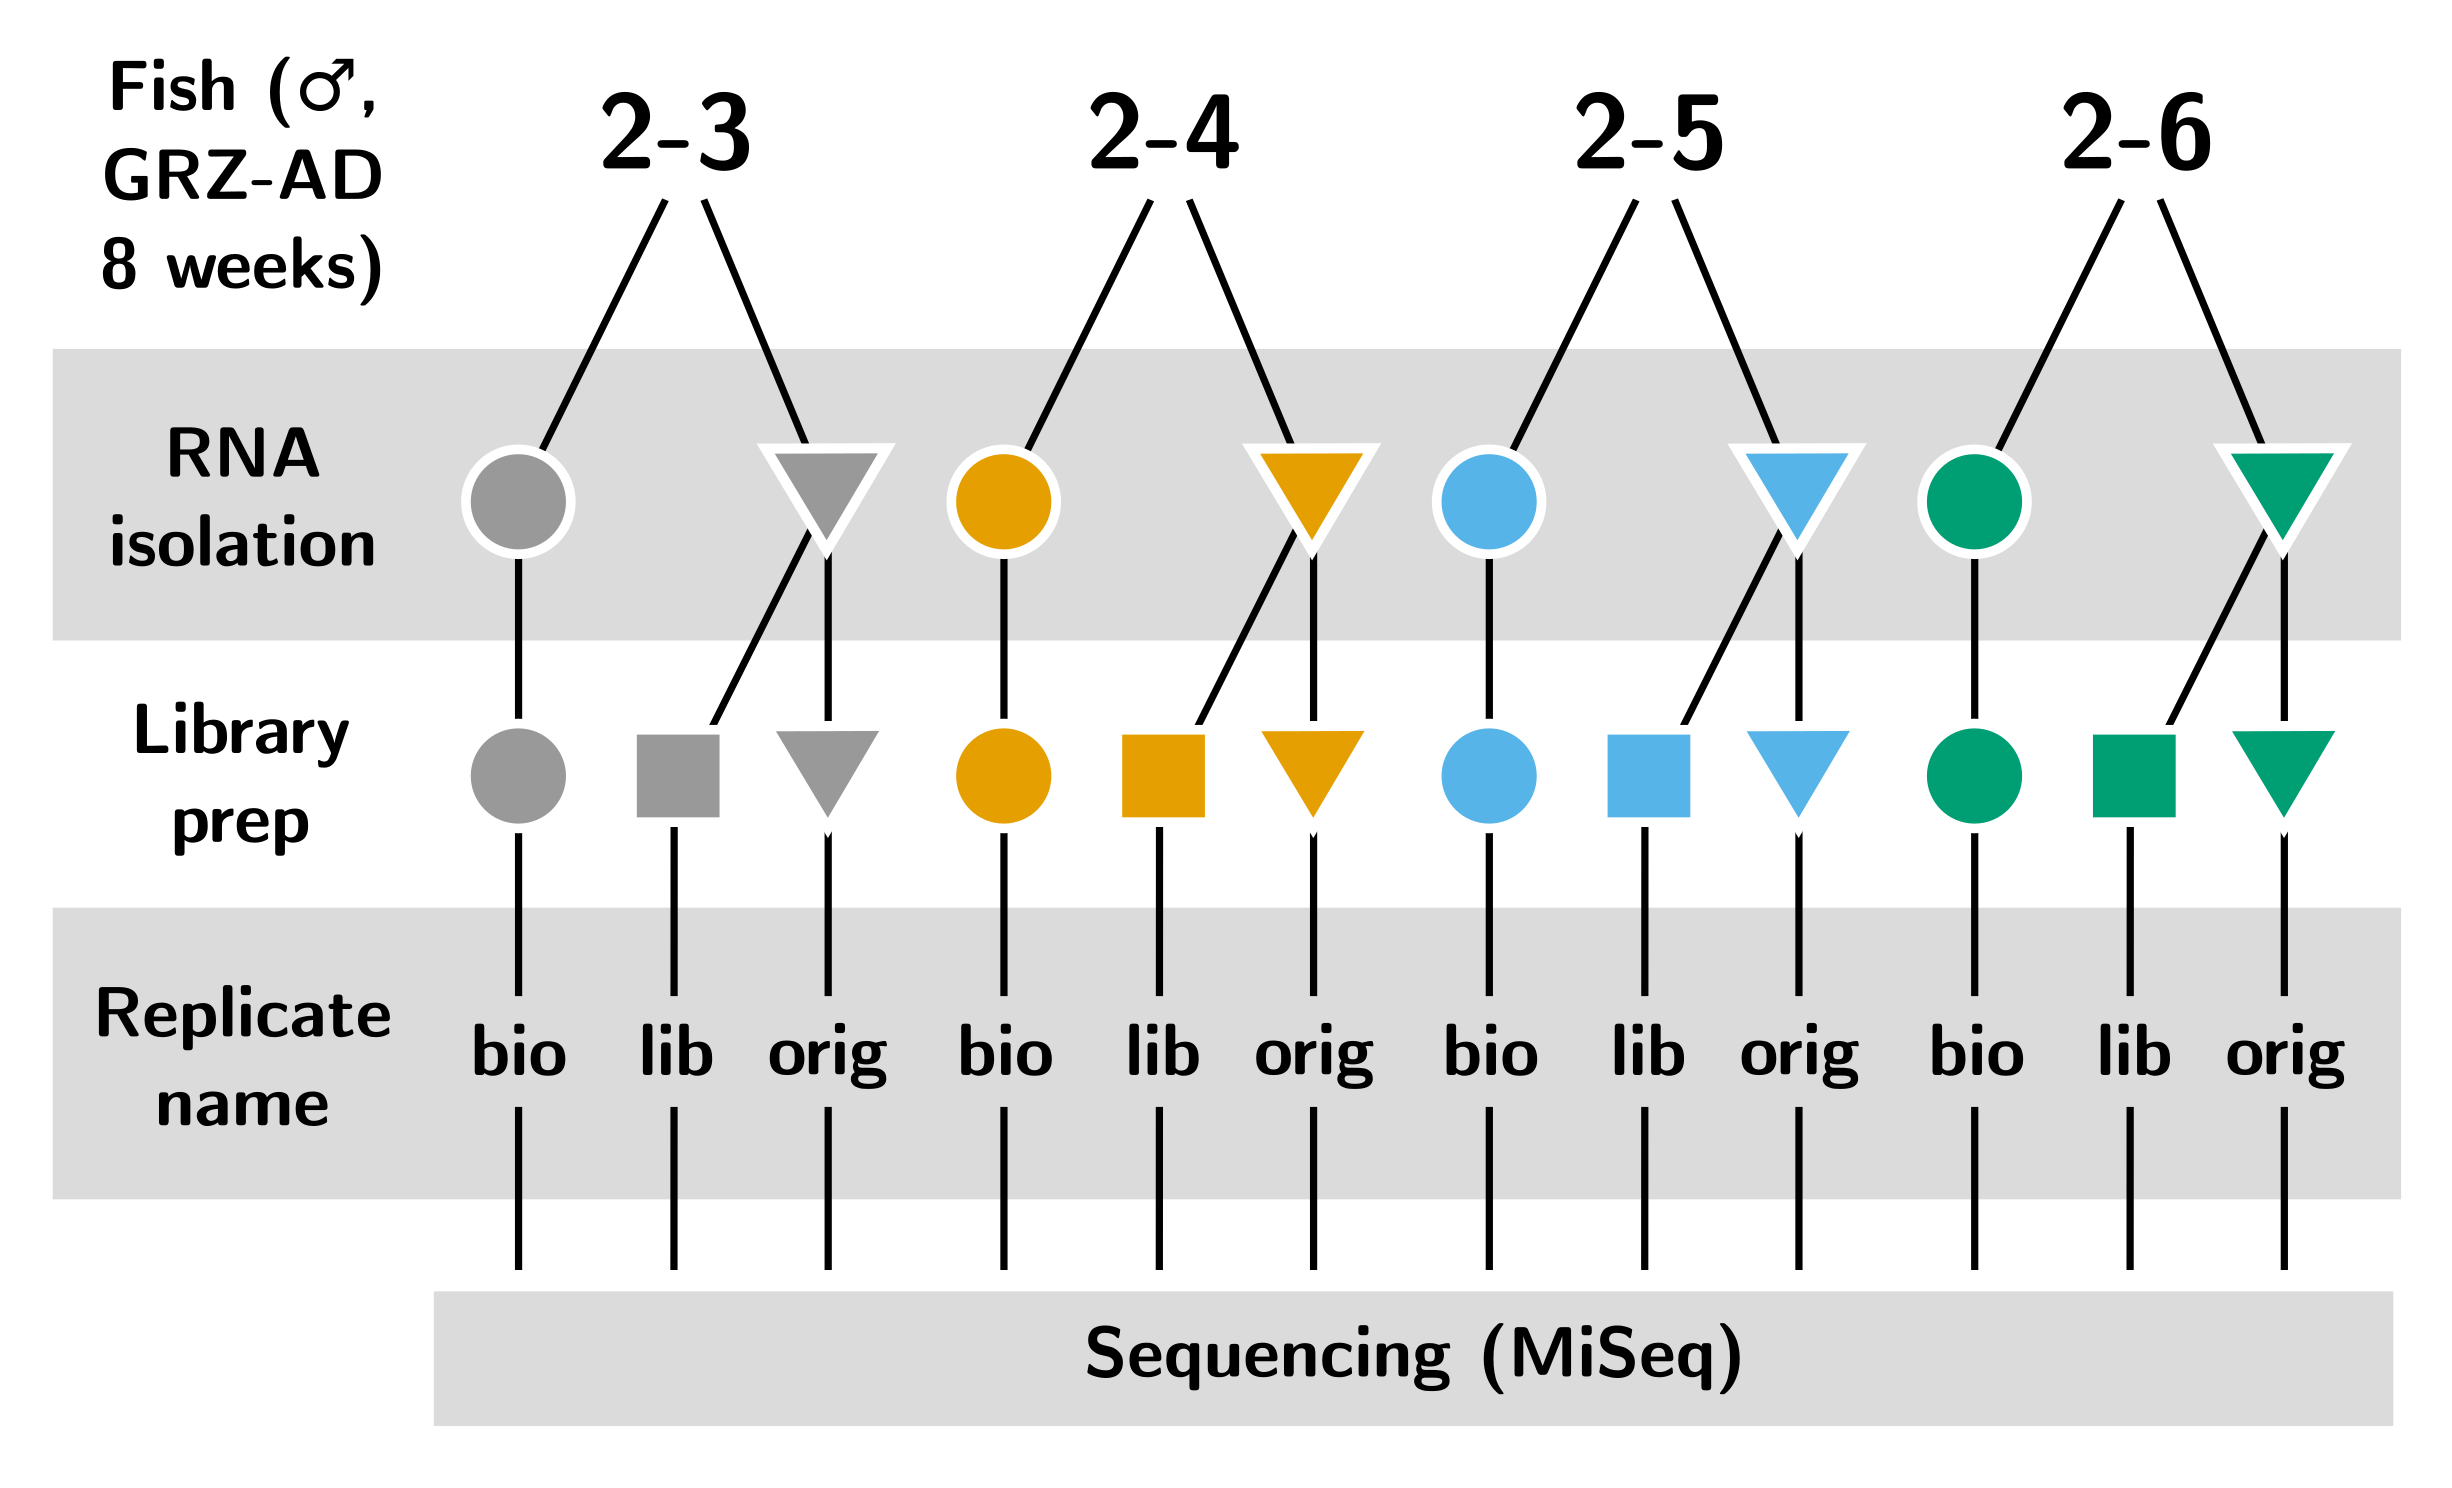
\includegraphics[width = 0.9\textwidth]{_Figures/png_edited/igseq-pilot-design_wide.png}
\caption{Experimental design of pilot study, showing relationship between replicates for each individual. Colour denotes individual of origin, while shape denotes replicate type.}
\label{fig:igseq-pilot-design}
\end{figure}

\subsection{Read survival and composition}
\label{sec:igseq_pilot_composition}

\Cref{fig:igseq-pilot-read-survival-init} shows the absolute and relative read survival for each of the twelve replicates throughout the pre-processing pipeline, up to and including VDJ assignment and Change-O table construction. The twelve replicates show relatively consistent behaviour, with \embed{_Figures/txt/pilot-read-survival-init-min.txt}\,\% to \embed{_Figures/txt/pilot-read-survival-init-max.txt}\,\% of reads surviving the entire process. Of those that do not, the biggest losses typically occur during quality filtering and removal of singleton sequences, with most other steps giving rise to relatively little sequence loss (\Cref{fig:igseq-pilot-read-survival-init-b}).

\begin{figure}
\centering
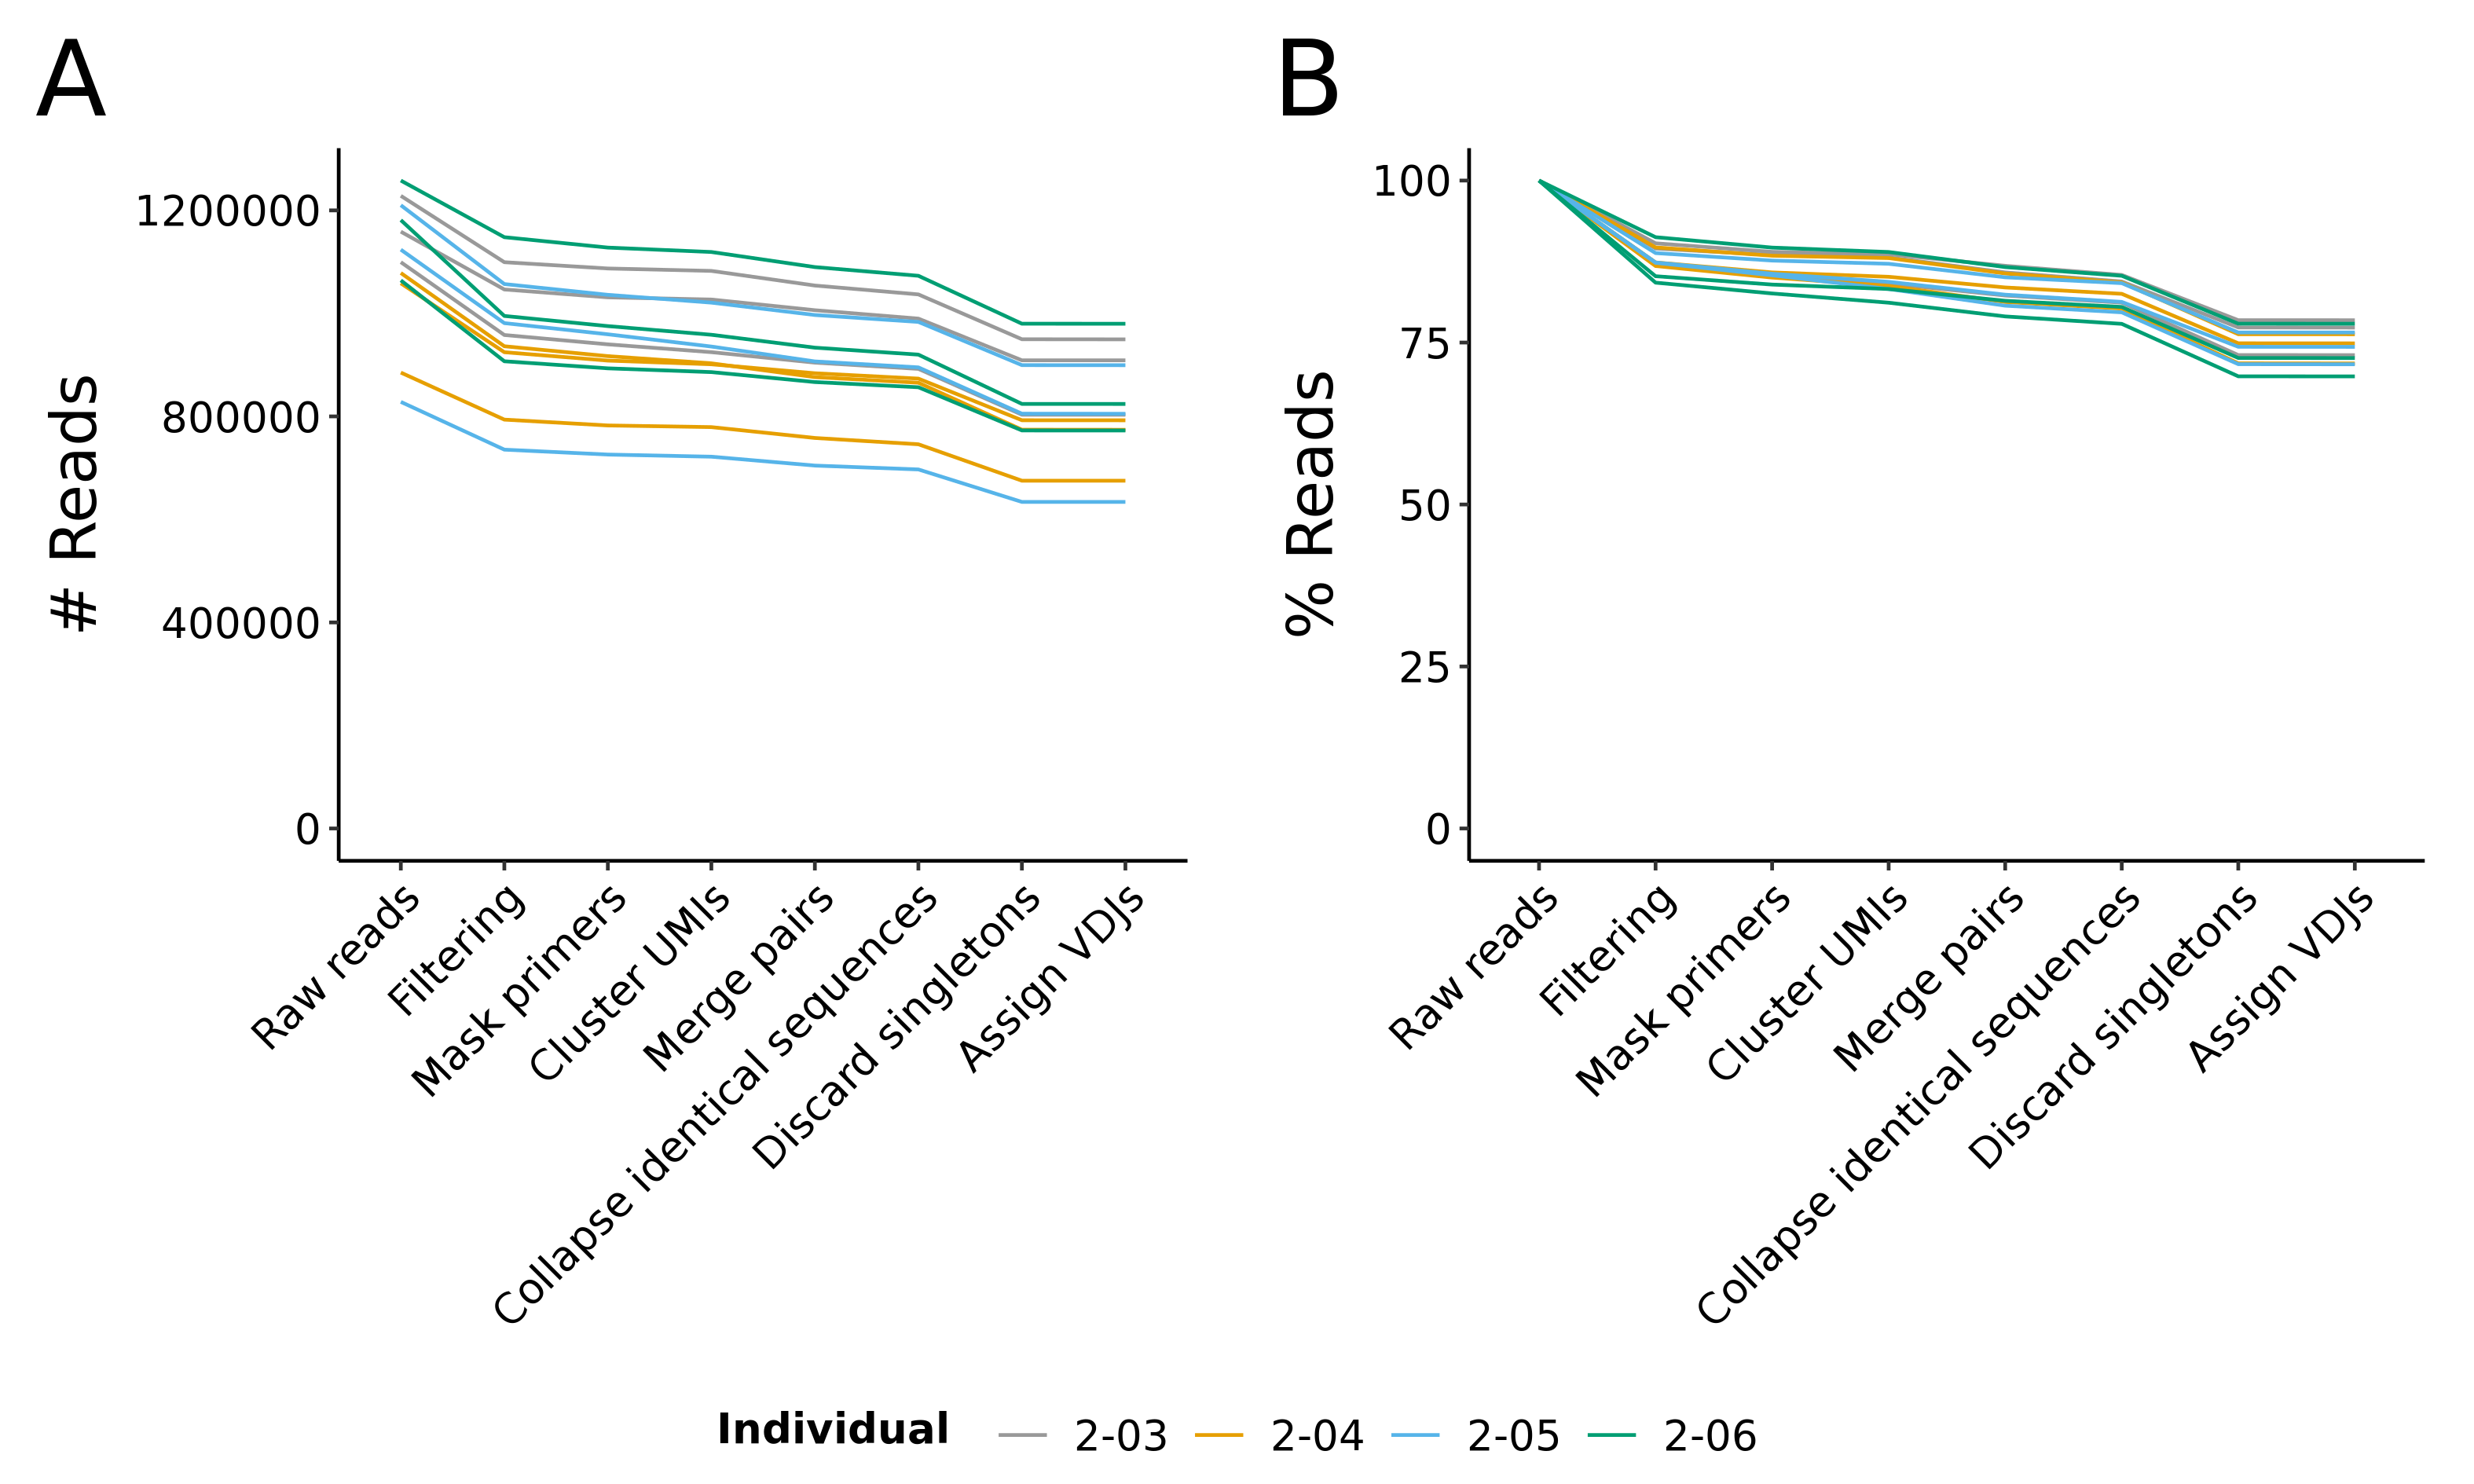
\includegraphics[width = 0.9\textwidth]{_Figures/png/pilot-read-survival-init.png}
\begin{subfigure}{0em}
\phantomsubcaption{}
\label{fig:igseq-pilot-read-survival-init-a}
\end{subfigure}
\begin{subfigure}{0em}
\phantomsubcaption{}
\label{fig:igseq-pilot-read-survival-init-b}
\end{subfigure}
\caption{Absolute (A) and relative (B) read survival during pre-processing of the pilot \igseq dataset, up to VDJ assignment and Change-O table construction.}
\label{fig:igseq-pilot-read-survival-init}
\end{figure}

In total, the pre-processed sequence repertoires of the pilot replicates contain between \embed{_Figures/txt/pilot-nseq-init-replicate-min.txt} and \embed{_Figures/txt/pilot-nseq-init-replicate-max.txt} unique sequences per replicate, corresponding to between \embed{_Figures/txt/pilot-nseq-init-individual-min.txt} and \embed{_Figures/txt/pilot-nseq-init-individual-max.txt} unique sequences per individual killifish and \embed{_Figures/txt/pilot-nseq-init-total.txt} unique sequences in total. Of these, \embed{_Figures/txt/pilot-nseq-init-pc-functional.txt}\,\% of sequences (corresponding to \embed{_Figures/txt/pilot-nreads-init-pc-functional.txt}\,\% of sequencing reads) are annotated by \program{Change-O} as functional, meaning they have successfully been assigned V- and J-identities, their V- and J-sequences are in-frame, and they do not contain any STOP codons (\Cref{fig:igseq-pilot-functional-prop-a}). A further \embed{_Figures/txt/pilot-nseq-init-pc-noj.txt}\,\% of sequences (corresponding to \embed{_Figures/txt/pilot-nreads-init-pc-noj.txt}\,\% of reads) failed to be assigned even an uncertain J-identity, meaning that no \jh sequence in the reference database aligned to the insert sequence; the remaining \embed{_Figures/txt/pilot-nseq-init-pc-other.txt}\,\% of sequences (corresponding to \embed{_Figures/txt/pilot-nreads-init-pc-other.txt}\,\% of reads) have a J-assignment but are rendered nonfunctional by an internal STOP codon and/or a frameshift between their V- and J-sequences (\Cref{fig:igseq-pilot-functional-prop-a}).

\begin{figure}
\centering
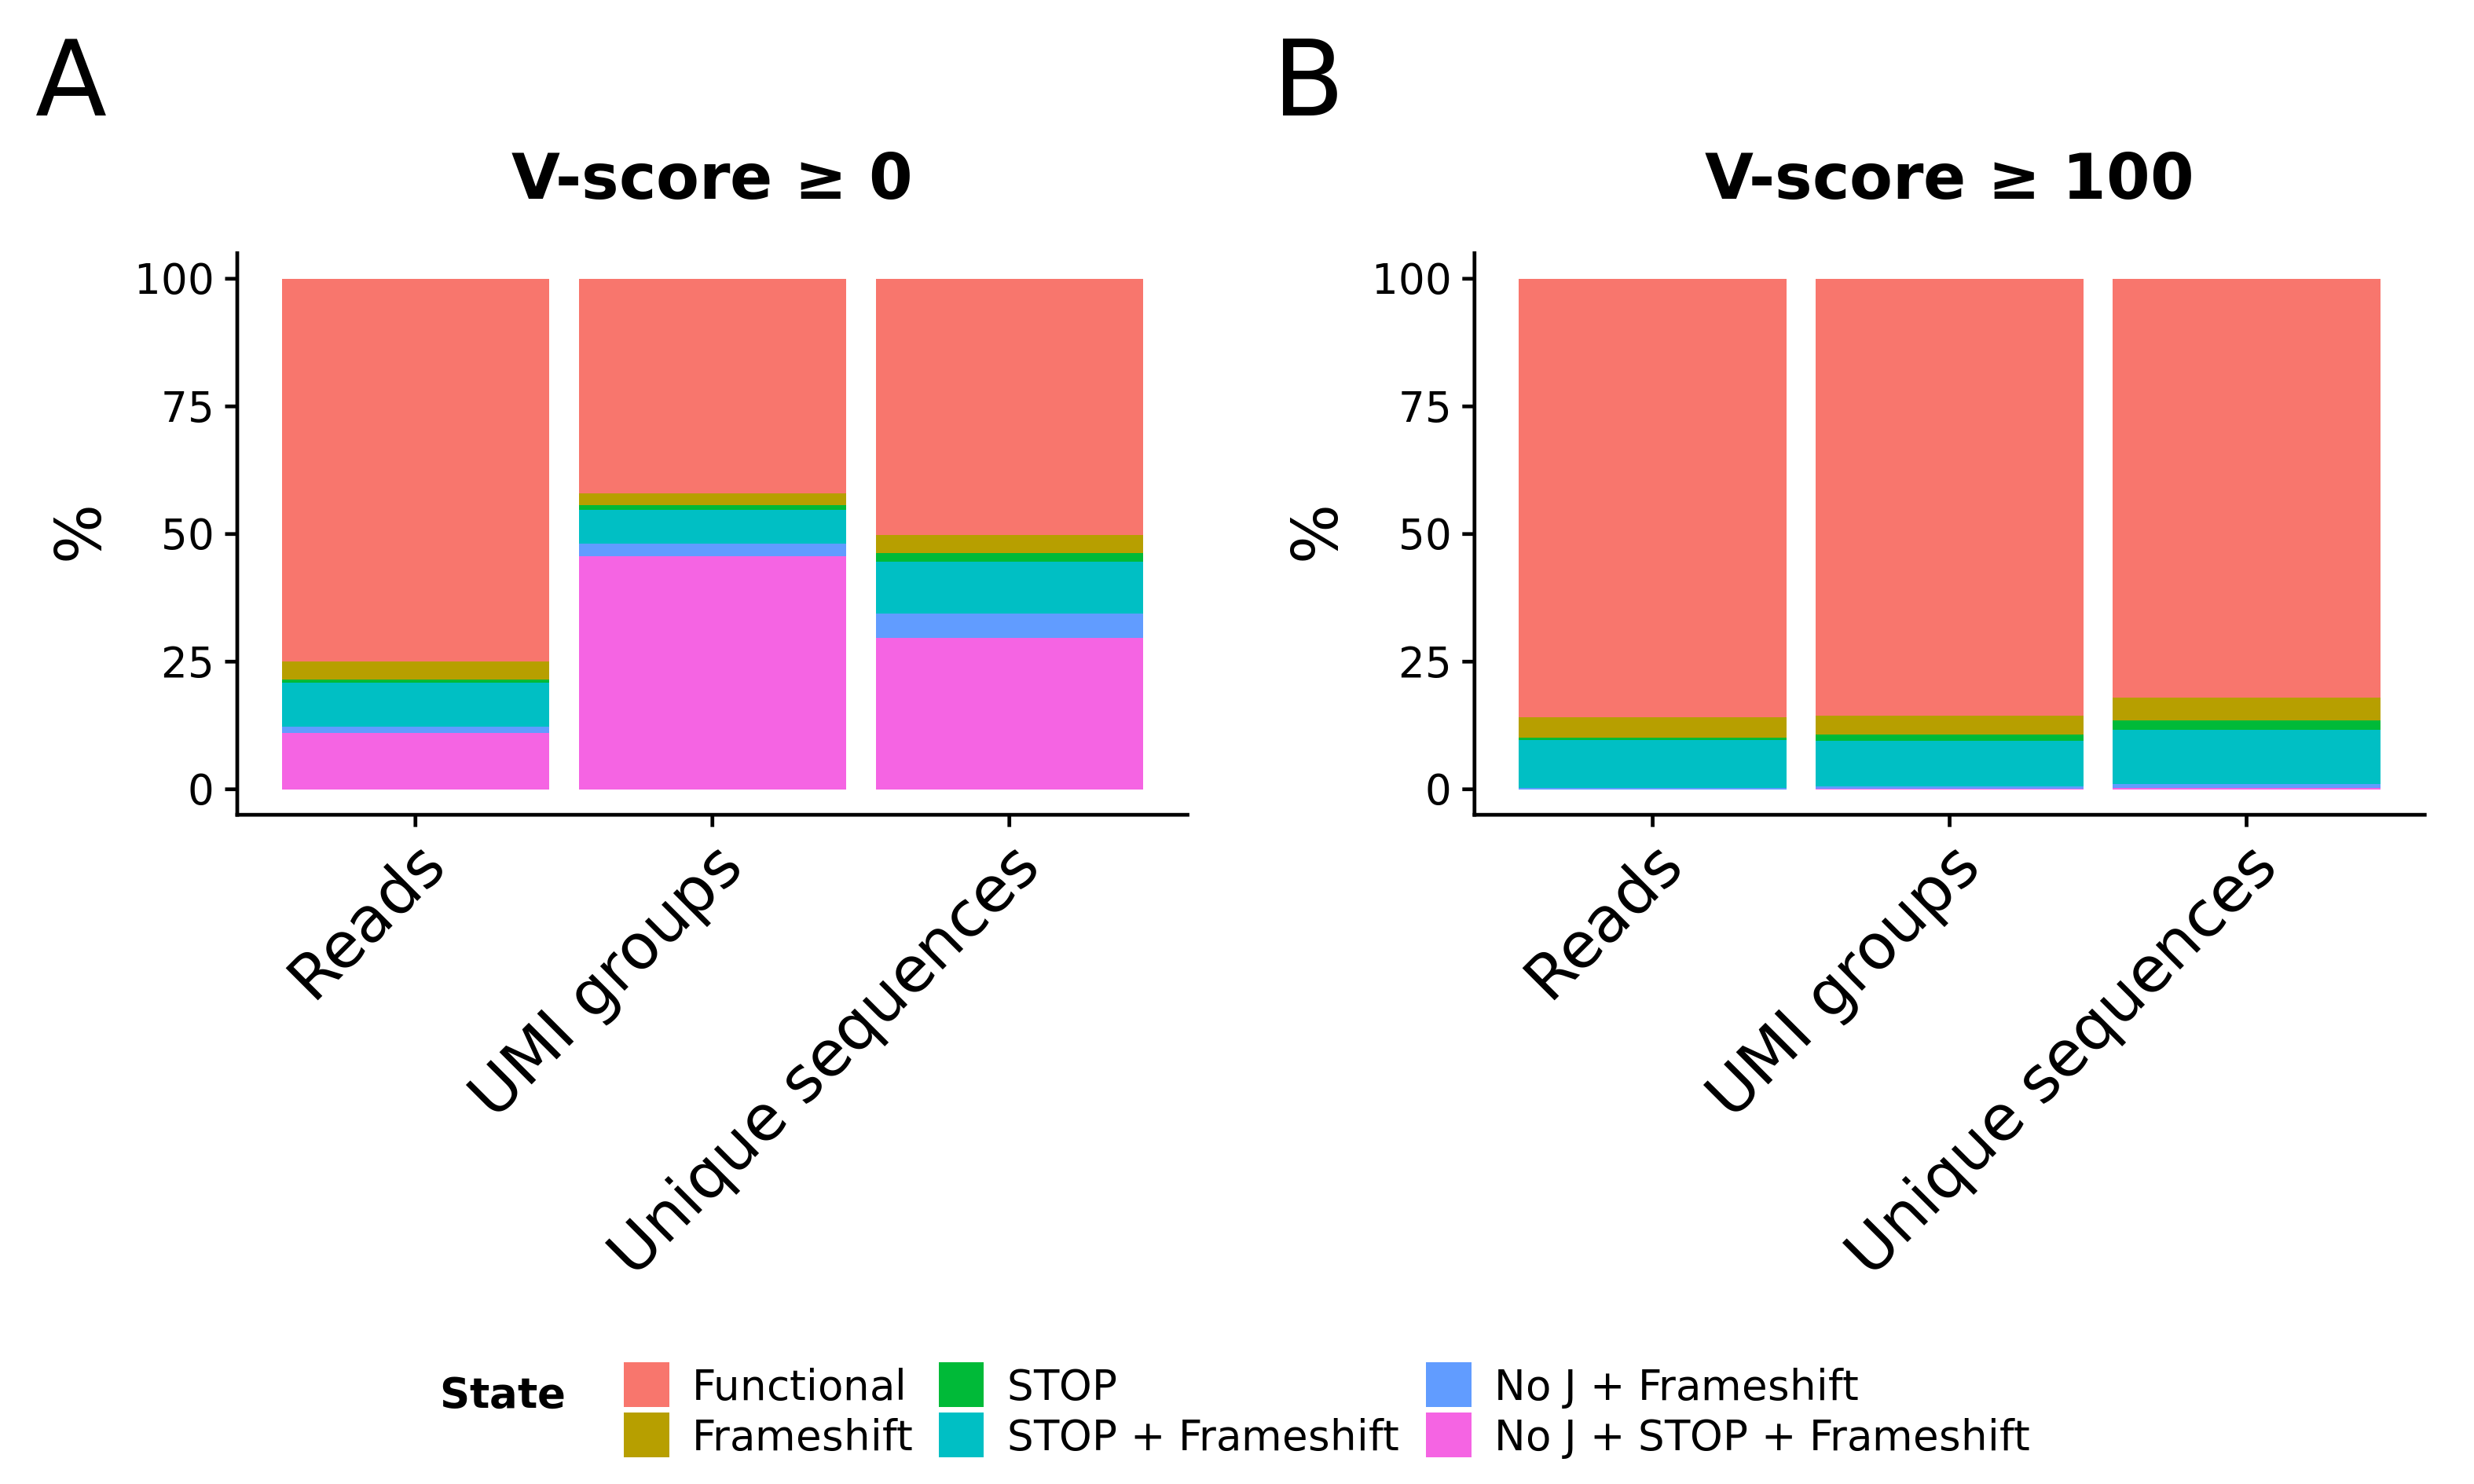
\includegraphics[width = 0.9\textwidth]{_Figures/png/pilot-functional-prop}
\begin{subfigure}{0em}
\phantomsubcaption{}
\label{fig:igseq-pilot-functional-prop-a}
\end{subfigure}
\begin{subfigure}{0em}
\phantomsubcaption{}
\label{fig:igseq-pilot-functional-prop-b}
\end{subfigure}
\caption{Proportion of input reads, UMI groups and unique sequences in the pilot \igseq dataset belonging to different (non)functional categories, before (A) and after (B) filtering on V-alignment score.}
\label{fig:igseq-pilot-functional-prop}
\end{figure}

As genuinely recombined but nonfunctional sequences would be expected to have undergone V(D)J recombination and so have a complete J-sequence, the lack of assigned J-identities for a significant minority of sequences suggests that this subset of sequences may be artefactual, erroneous or otherwise malformed. Supporting this assumption, sequences without J-assignments overwhelmingly have very low V-alignment scores reported by \program{IgBLAST}, with an average score of \embed{_Figures/txt/pilot-vscore-mean-noj.txt} $\pm$ \embed{_Figures/txt/pilot-vscore-sd-noj.txt} (mean $\pm$ standard deviation), compared to \embed{_Figures/txt/pilot-vscore-mean-other.txt} $\pm$ \embed{_Figures/txt/pilot-vscore-sd-other.txt} for other nonfunctional sequences and \embed{_Figures/txt/pilot-vscore-mean-functional.txt} $\pm$ \embed{_Figures/txt/pilot-vscore-sd-functional.txt} for functional sequences (\Cref{fig:igseq-pilot-functional-vscores}). A simple V-score cut-off of 100, therefore, effectively removes the vast majority of these low-quality sequences, while leaving the population of functional sequences intact (\Cref{fig:igseq-pilot-functional-prop-b}).

\begin{figure}
\centering
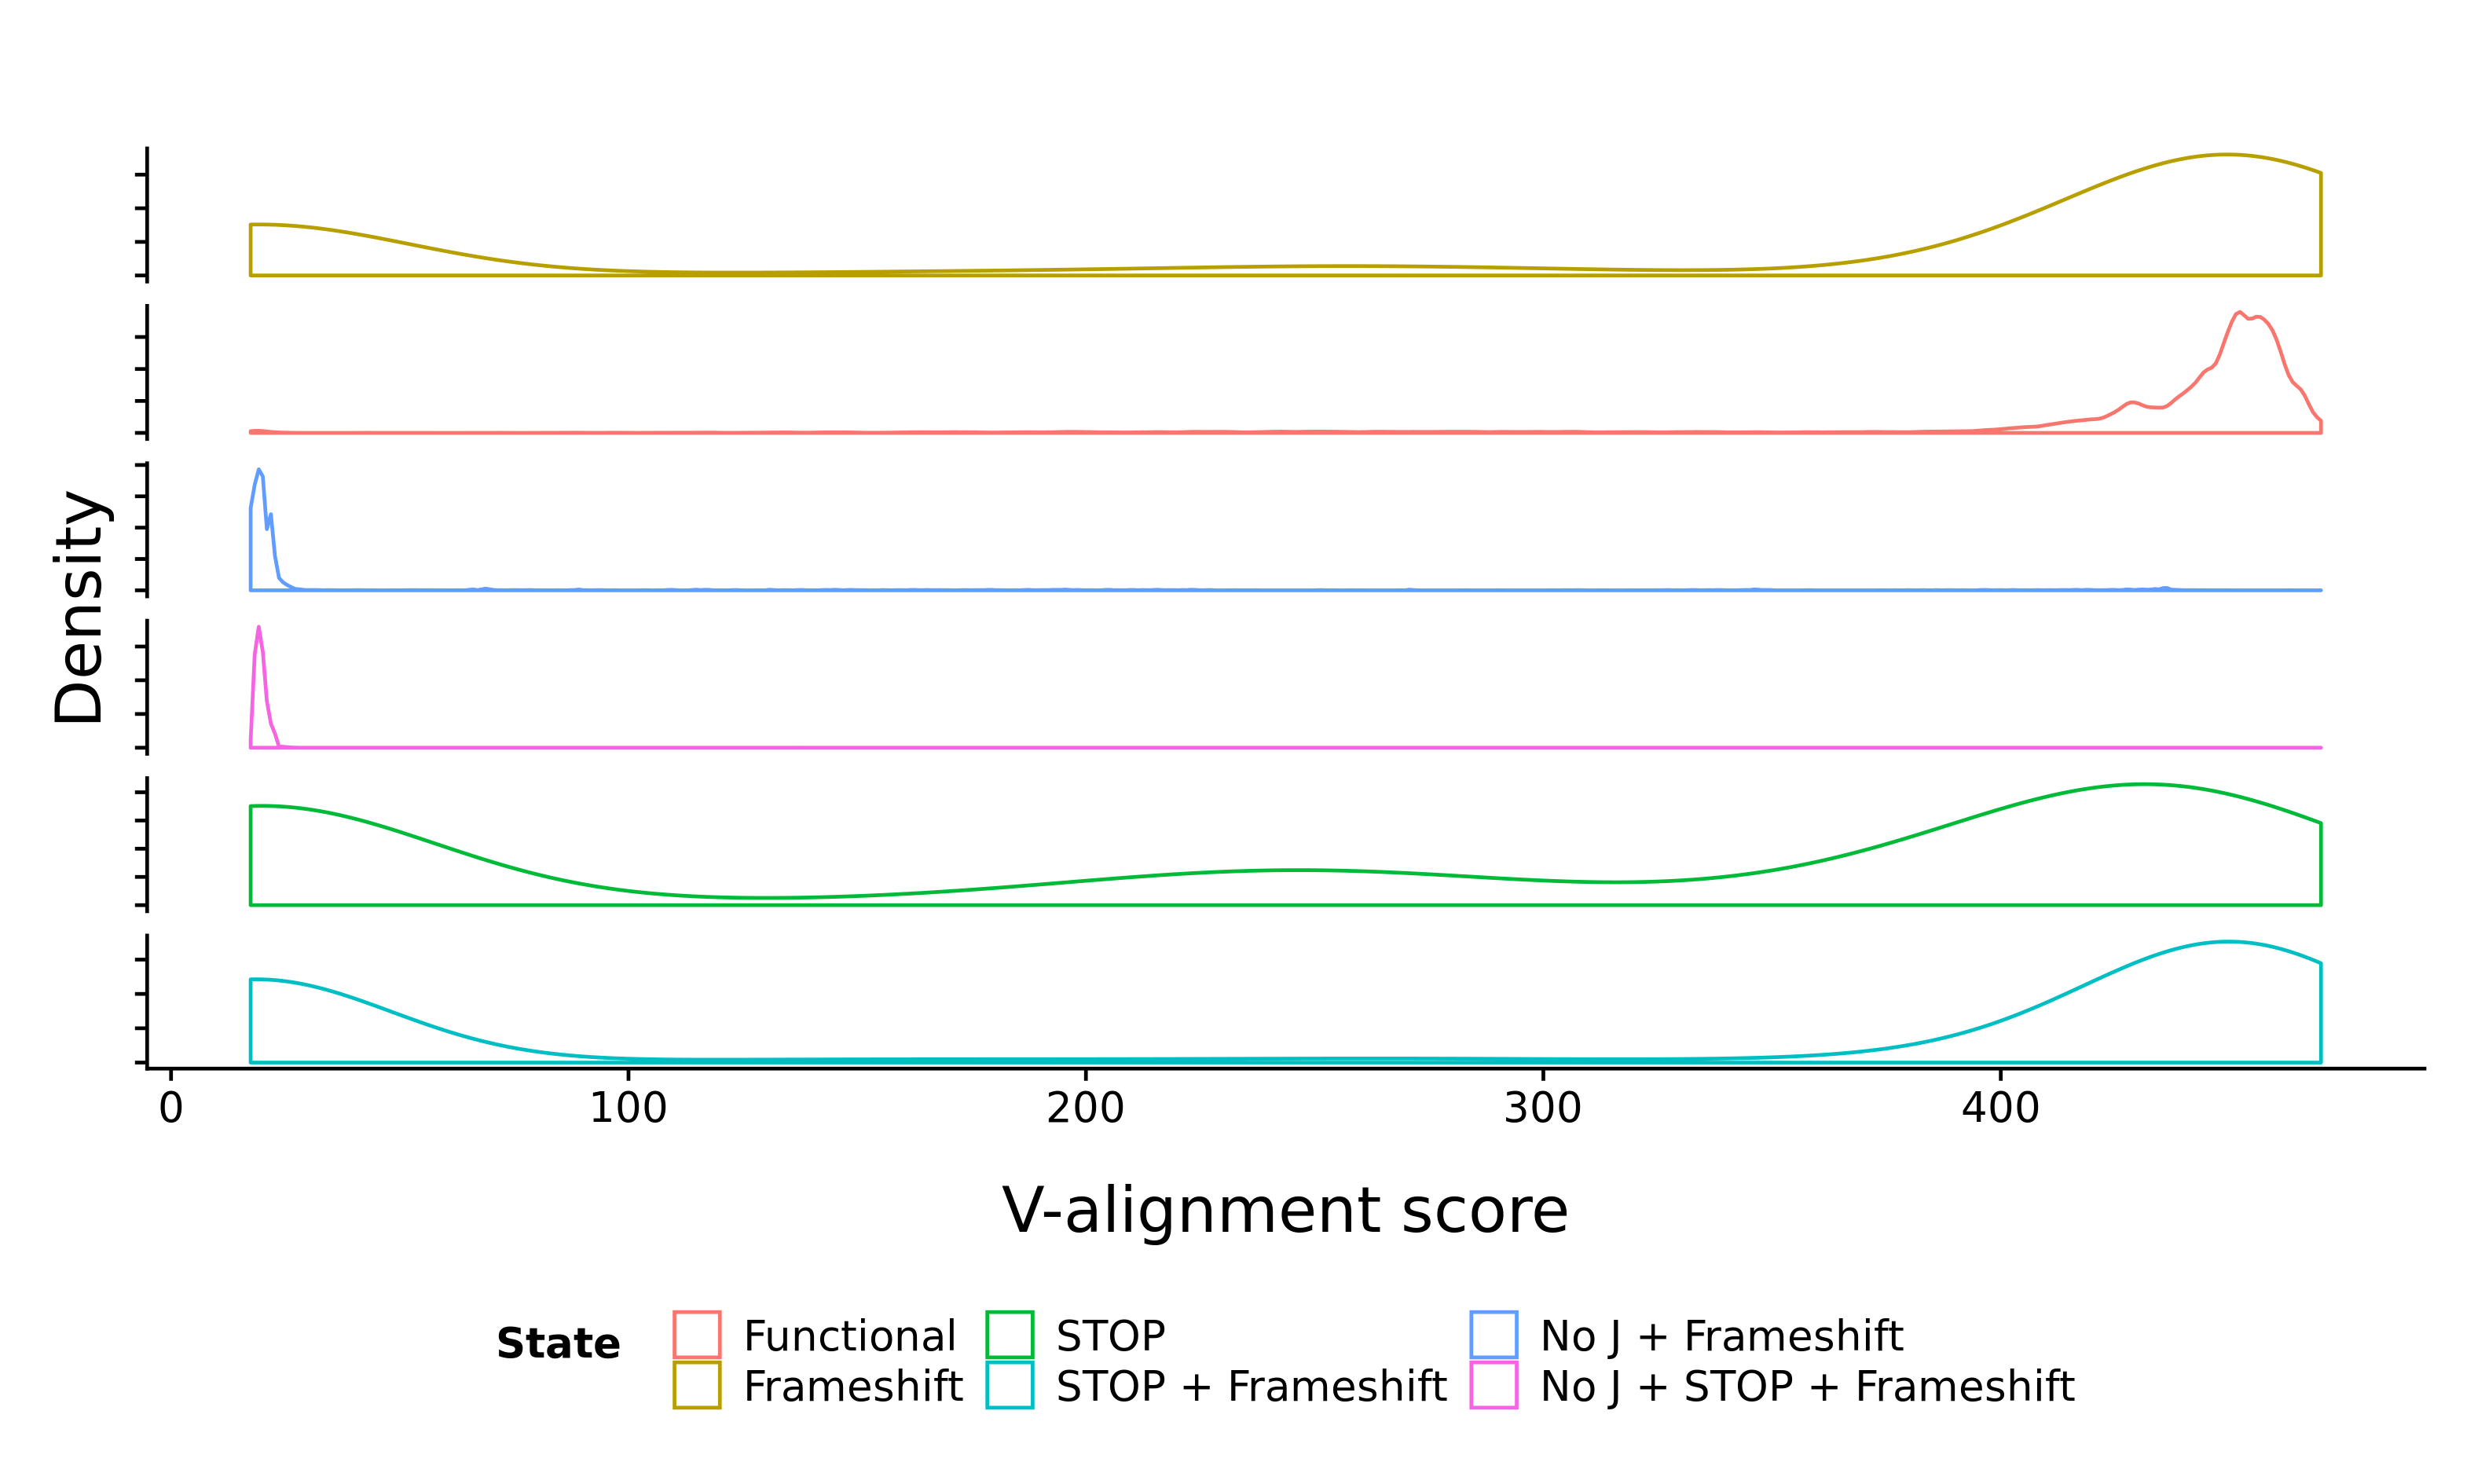
\includegraphics[width = 0.9\textwidth]{_Figures/png/pilot-functional-vscores}
\caption{Kernel density plots of distributions of V-alignment scores among unique sequences in the pilot \igseq dataset. Vertical axes are not to scale between sequence categories.}
\label{fig:igseq-pilot-functional-vscores}
\end{figure}

In total, \embed{_Figures/txt/pilot-nseq-init-dropped-vscore.txt} unique sequences, corresponding to \embed{_Figures/txt/pilot-read-survival-rel-loss-total.txt}\,\% of input reads, were removed in this way. As a result, including this final filtering step, between \embed{_Figures/txt/pilot-read-survival-all-min.txt}\,\% and \embed{_Figures/txt/pilot-read-survival-all-max.txt}\,\% of reads per input library survived the complete pre-processing process (\Cref{fig:igseq-pilot-read-survival-all}), a good range suggesting both that the library-preparation protocol successfully captured antibody-repertoire sequencing data from turquoise killifish for the first time, and that the subsequent computational pipeline was able to completely and successfully process the majority of the resulting data. Of the remaining \embed{_Figures/txt/pilot-nseq-init-kept-vscore.txt} unique sequences present in the dataset, \embed{_Figures/txt/pilot-nseq-init-functional-filtered.txt} (\embed{_Figures/txt/pilot-nseq-init-pc-functional-filtered.txt}\,\%) are functional, \embed{_Figures/txt/pilot-nseq-init-other-filtered.txt} (\embed{_Figures/txt/pilot-nseq-init-pc-other-filtered.txt}\,\%) are rendered nonfunctional by a STOP codon or frameshift, and only \embed{_Figures/txt/pilot-nseq-init-noj-filtered.txt} (\embed{_Figures/txt/pilot-nseq-init-pc-noj-filtered.txt}\,\%) could not be assigned a J-identity (\Cref{fig:igseq-pilot-functional-prop-b}). These results confirm that the data from this first \igseq experiment in the turquoise killifish are of sufficient quality to proceed to clonotyping and analysis of repertoire diversity.

\begin{figure}
\centering
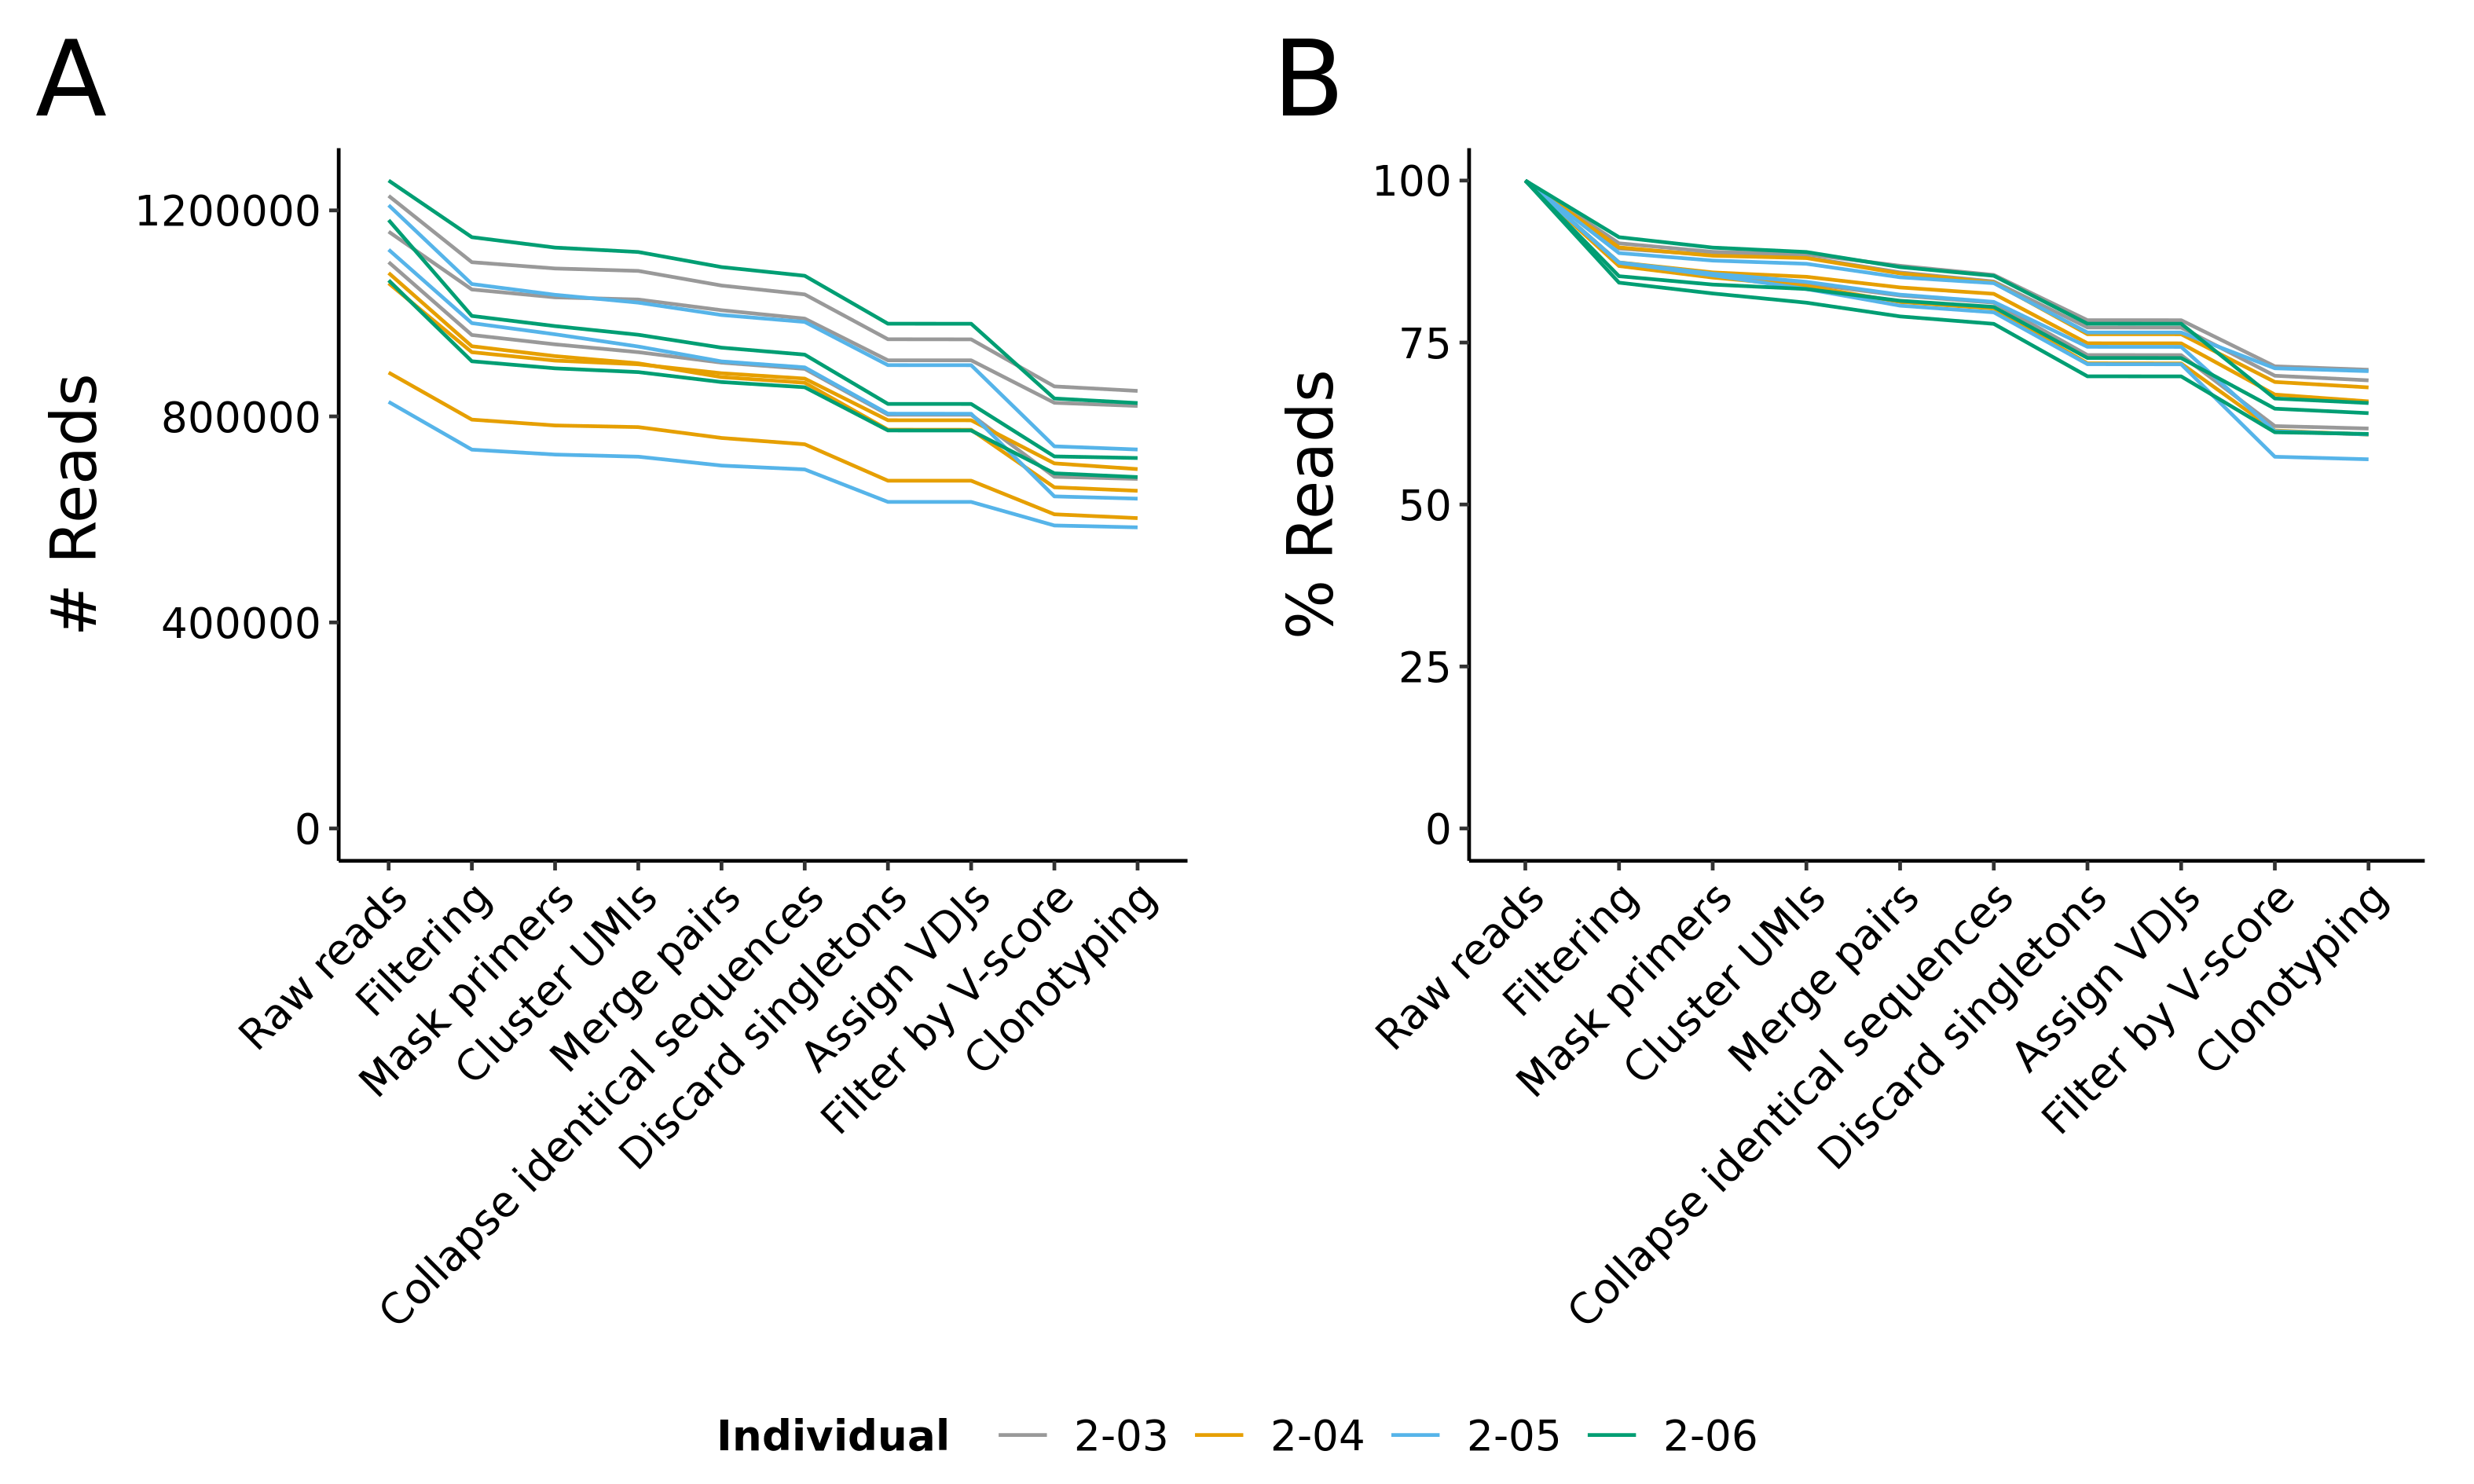
\includegraphics[width = 0.9\textwidth]{_Figures/png/pilot-read-survival-all.png}
\begin{subfigure}{0em}
\phantomsubcaption{}
\label{fig:igseq-pilot-read-survival-all-a}
\end{subfigure}
\begin{subfigure}{0em}
\phantomsubcaption{}
\label{fig:igseq-pilot-read-survival-all-b}
\end{subfigure}
\caption{Absolute (A) and relative (B) read survival during pre-processing of the pilot \igseq dataset, up to and including clonotyping.}
\label{fig:igseq-pilot-read-survival-all}
\end{figure}

\subsection{Clonotyping and clonal repertoire diversity}
\label{sec:igseq_pilot_clones}

Following assignment of VDJ identities and quality filtering, sequences in an antibody repertoire can be assigned to clones: groups of B-cells descended from a single \naive B-cell ancestor, and therefore sharing a single VDJ-recombination event. Sequences in the same clone are said to share a \textit{clonotype}. In \program{Change-O}, clonotyping is performed by dividing sequences into groups sharing a consistent V-assignment, J-assignment and CDR3 length, then performing single-linkage clustering on each group of sequences based on Hamming distances between CDR3 sequences \parencite{gupta2017hierarchical}. To identify a distance threshold for cutting the cluster dendrogram into clones, each unique sequence in the repertoire is assigned a nearest-neighbour distance based on the length-normalised Hamming distance to the most similar sequence in the repertoire. The resulting nearest-neighbour distance is typically bimodal, with the lower peak (representing more-similar sequences) indicating members of the same clonotype and the higher peak (representing less-similar sequences) indicating members of different clones; by fitting a pair of gamma or normal distributions to these two peaks, a distance threshold for clonotype membership can be determined according to the desired levels of sensitivity and specificity \parencite{nouri2018threshold} (\Cref{sec:methods_comp_igpreproc_clones}). By cutting the cluster dendrogram at this threshold, each group of repertoire sequences can be separated into some number of distinct clones, each of which shares a unique \naive B-cell ancestor.
% TODO: Figure describing clonotyping process?

One disadvantage of single-linkage clustering in this context is that non-informative \sequence{N} positions can result in artifactual links between unrelated sequences. As such, sequences with a large number of junctional \sequence{N} positions can significantly disrupt the clonotyping process. On the other hand, as over \embed{_Figures/txt/pilot-filtered-nn-any.txt}\,\% of unique sequences in the pilot dataset contain at least one such junctional \sequence{N} position, excluding them all would represent a significant loss of data. In order to minimise the number of discarded sequences while also minimising the disrupting effects of sequences with junctional \sequence{N}s, sequences with exactly one junctional \sequence{N} position (comprising \embed{_Figures/txt/pilot-filtered-1n-total.txt}\,\% of total sequences and \embed{_Figures/txt/pilot-filtered-1n-withn.txt}\,\% of sequences with at least one junctional \sequence{N}; \Cref{tab:igseq-pilot-filtered-nn}) were included in the clonotyping process for the pilot dataset, while those with two or more junctional \sequence{N} positions were excluded. This procedure successfully assigned clonal identities to \embed{_Figures/txt/pilot-nseq-assigned-clones.txt}\,\% of unique sequences in the V-score-filtered dataset, with fewer than \embed{_Figures/txt/pilot-nseq-lost-clonotyping.txt} sequences (corresponding to \embed{_Figures/txt/pilot-pc-reads-lost-clonotyping.txt}\,\% of input reads) lost during the clonotyping phase of the pipeline.

\begin{table}
\caption{Distribution of junctional \sequence{N} positions in the V-score-filtered pilot dataset.}
\label{tab:igseq-pilot-filtered-nn}
% latex table generated in R 3.5.2 by xtable 1.8-3 package
% Wed Apr  3 14:27:33 2019
\begin{tabular}{lrrr}
  \toprule \# junctional Ns & \# unique sequences & \% of all sequences & \% of sequences with $>$0 junctional Ns \\ 
  \midrule 0 & 49134 & 88.924 & 0.00 \\ 
  1 & 3388 & 6.132 & 67.94 \\ 
  2 & 961 & 1.739 & 19.27 \\ 
  3 & 324 & 0.586 & 6.50 \\ 
  4 & 125 & 0.226 & 2.51 \\ 
  5 & 93 & 0.168 & 1.86 \\ 
  $>$5 & 96 & 0.174 & 1.93 \\ 
   \bottomrule \end{tabular}

\end{table}

In total, \embed{_Figures/txt/pilot-nclones-individual-min.txt} to \embed{_Figures/txt/pilot-nclones-individual-max.txt} clones were identified per individual fish in the pilot dataset. As expected, the clone-size distribution is overwhelmingly dominated by small clones (\Cref{fig:igseq-pilot-clone-sizes-sizes}): across all individuals, \embed{_Figures/txt/pilot-nclones-pc-1count.txt}\,\% of clones are observed as just a single unique sequence across all replicates, while \embed{_Figures/txt/pilot-nclones-pc-small.txt}\,\% contain fewer than five unique sequences. As a result, the great majority of clones (\embed{_Figures/txt/pilot-nclones-pc-1rep.txt}\,\%) are observed in only a single replicate per individual, with \embed{_Figures/txt/pilot-nclones-pc-2rep.txt}\,\% present in two replicates and only  \embed{_Figures/txt/pilot-nclones-pc-3rep.txt}\,\% shared across all three. Unsurprisingly, however, larger clones are much more likely to be shared across multiple replicates (\Cref{fig:igseq-pilot-clone-sizes-reps}), consistent with a model in which a very large number of small clones are sampled only rarely while a much smaller number of large clones is sampled much more often \parencite{mora2016diversity}. Overall, the level of agreement between the replicates is high (\Cref{fig:igseq-pilot-clone-sizes-cor-boxplots,fig:igseq-pilot-clone-sizes-cor-scatter}), with an average inter-replicate correlation in clone size of $r=\embed{_Figures/txt/pilot-clone-sizes-cor-avg.txt}$, indicating that, despite the problem of undersampling many very small clones, the clonal composition of the killifish can be captured reproducibly by \Igseq.

\begin{figure}
\centering
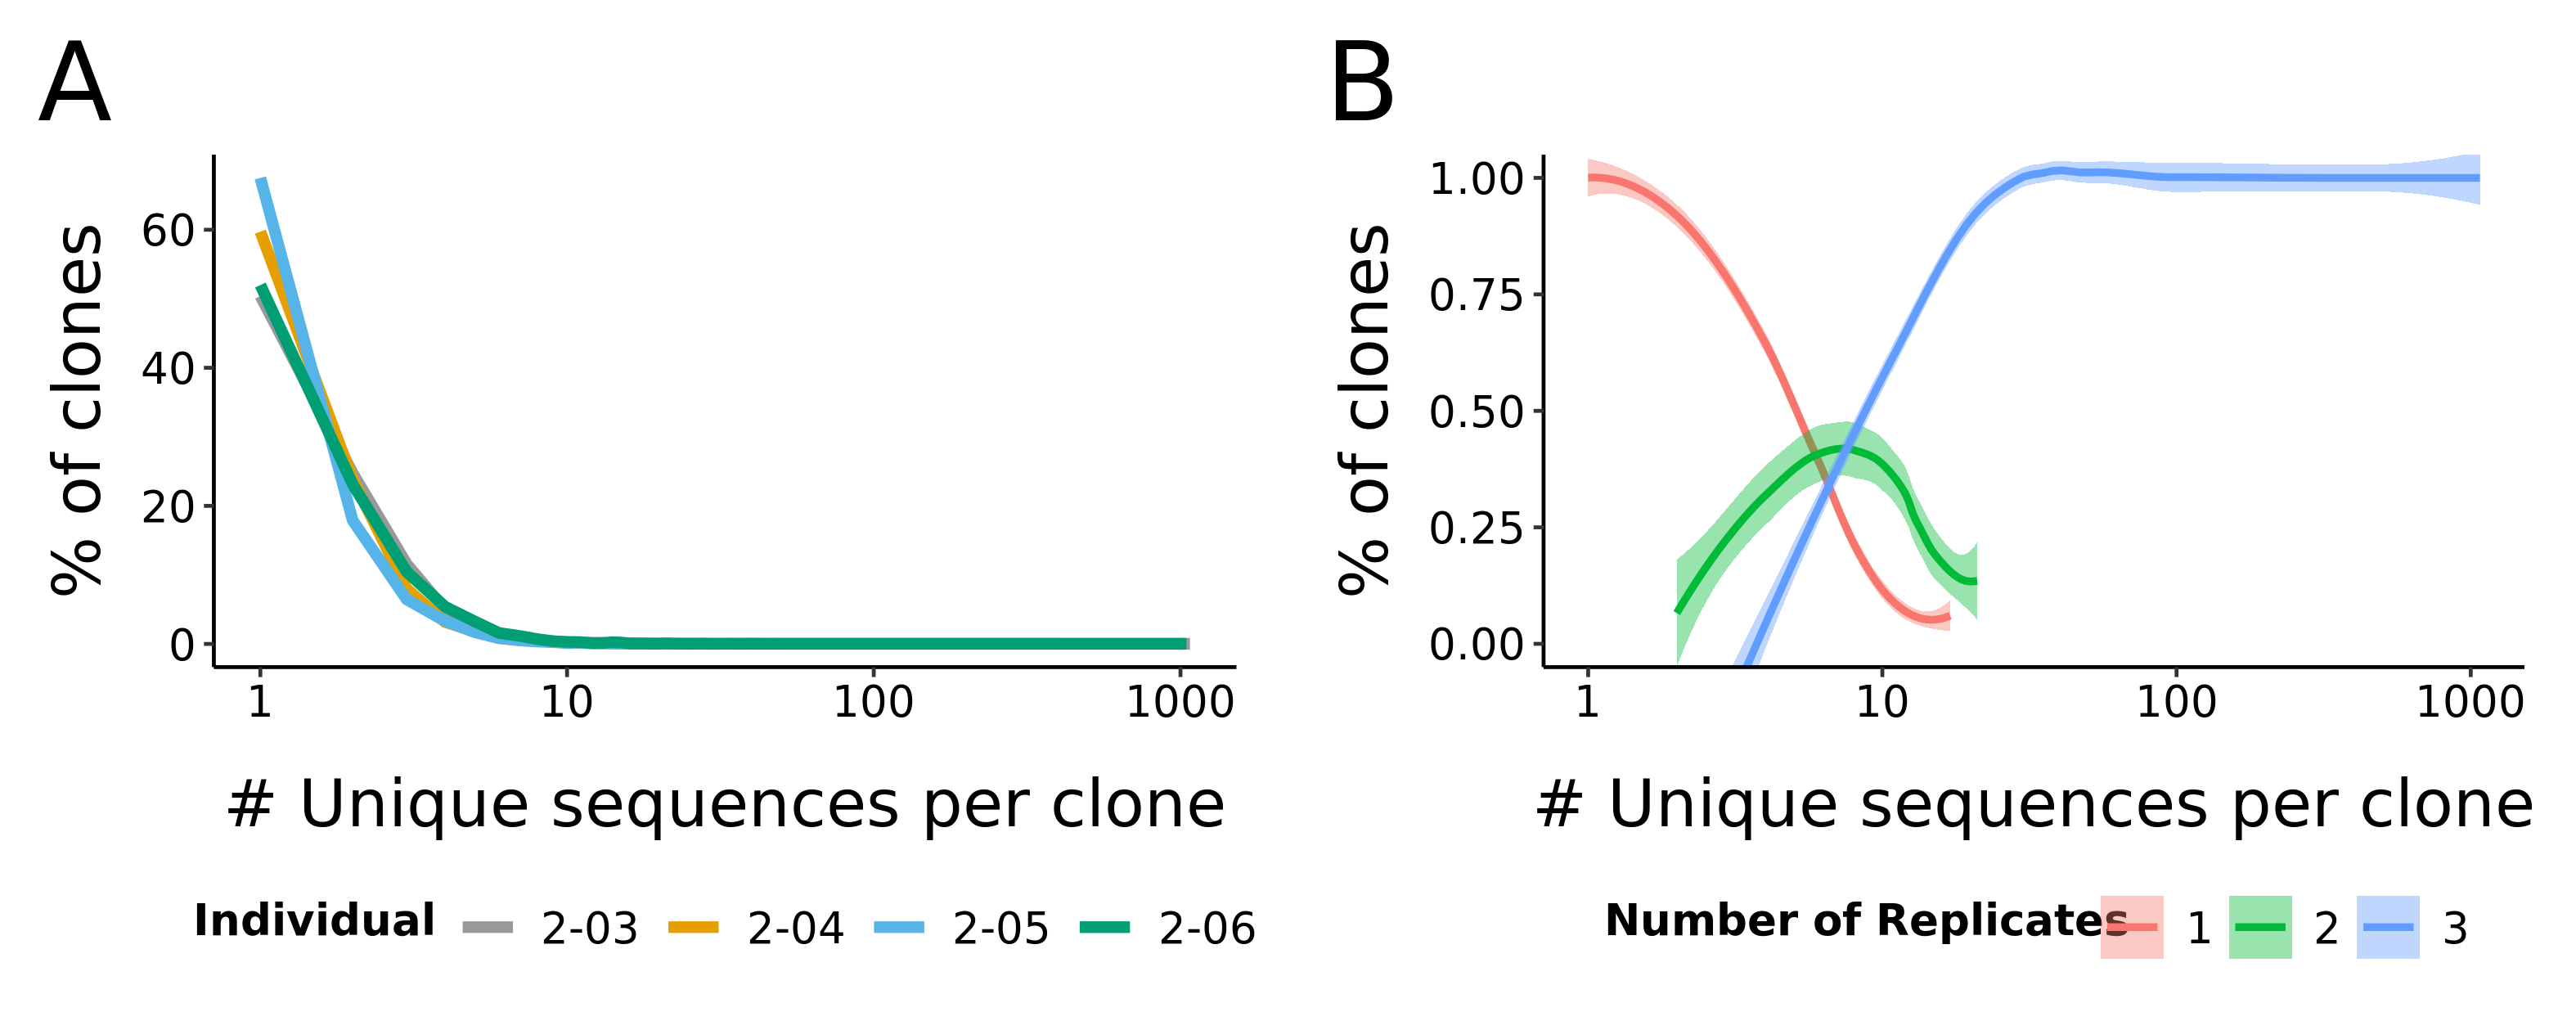
\includegraphics[width = 0.9\textwidth]{_Figures/png/pilot-clone-sizes}
\begin{subfigure}{0em}
\phantomsubcaption{}
\label{fig:igseq-pilot-clone-sizes-sizes}
\end{subfigure}
\begin{subfigure}{0em}
\phantomsubcaption{}
\label{fig:igseq-pilot-clone-sizes-reps}
\end{subfigure}
\caption{(A) Proportion of clones of different sizes for each individual in the pilot dataset, measured in unique sequences per clone. (B) LOESS-smoothed curves showing proportion of clones of each size found across one, two or all three replicates of the appropriate individual.}
% TODO: Add suitable overall figure title
\label{fig:igseq-pilot-clone-sizes}
\end{figure} % TODO: cite LOESS smoothing

\begin{figure}
\centering
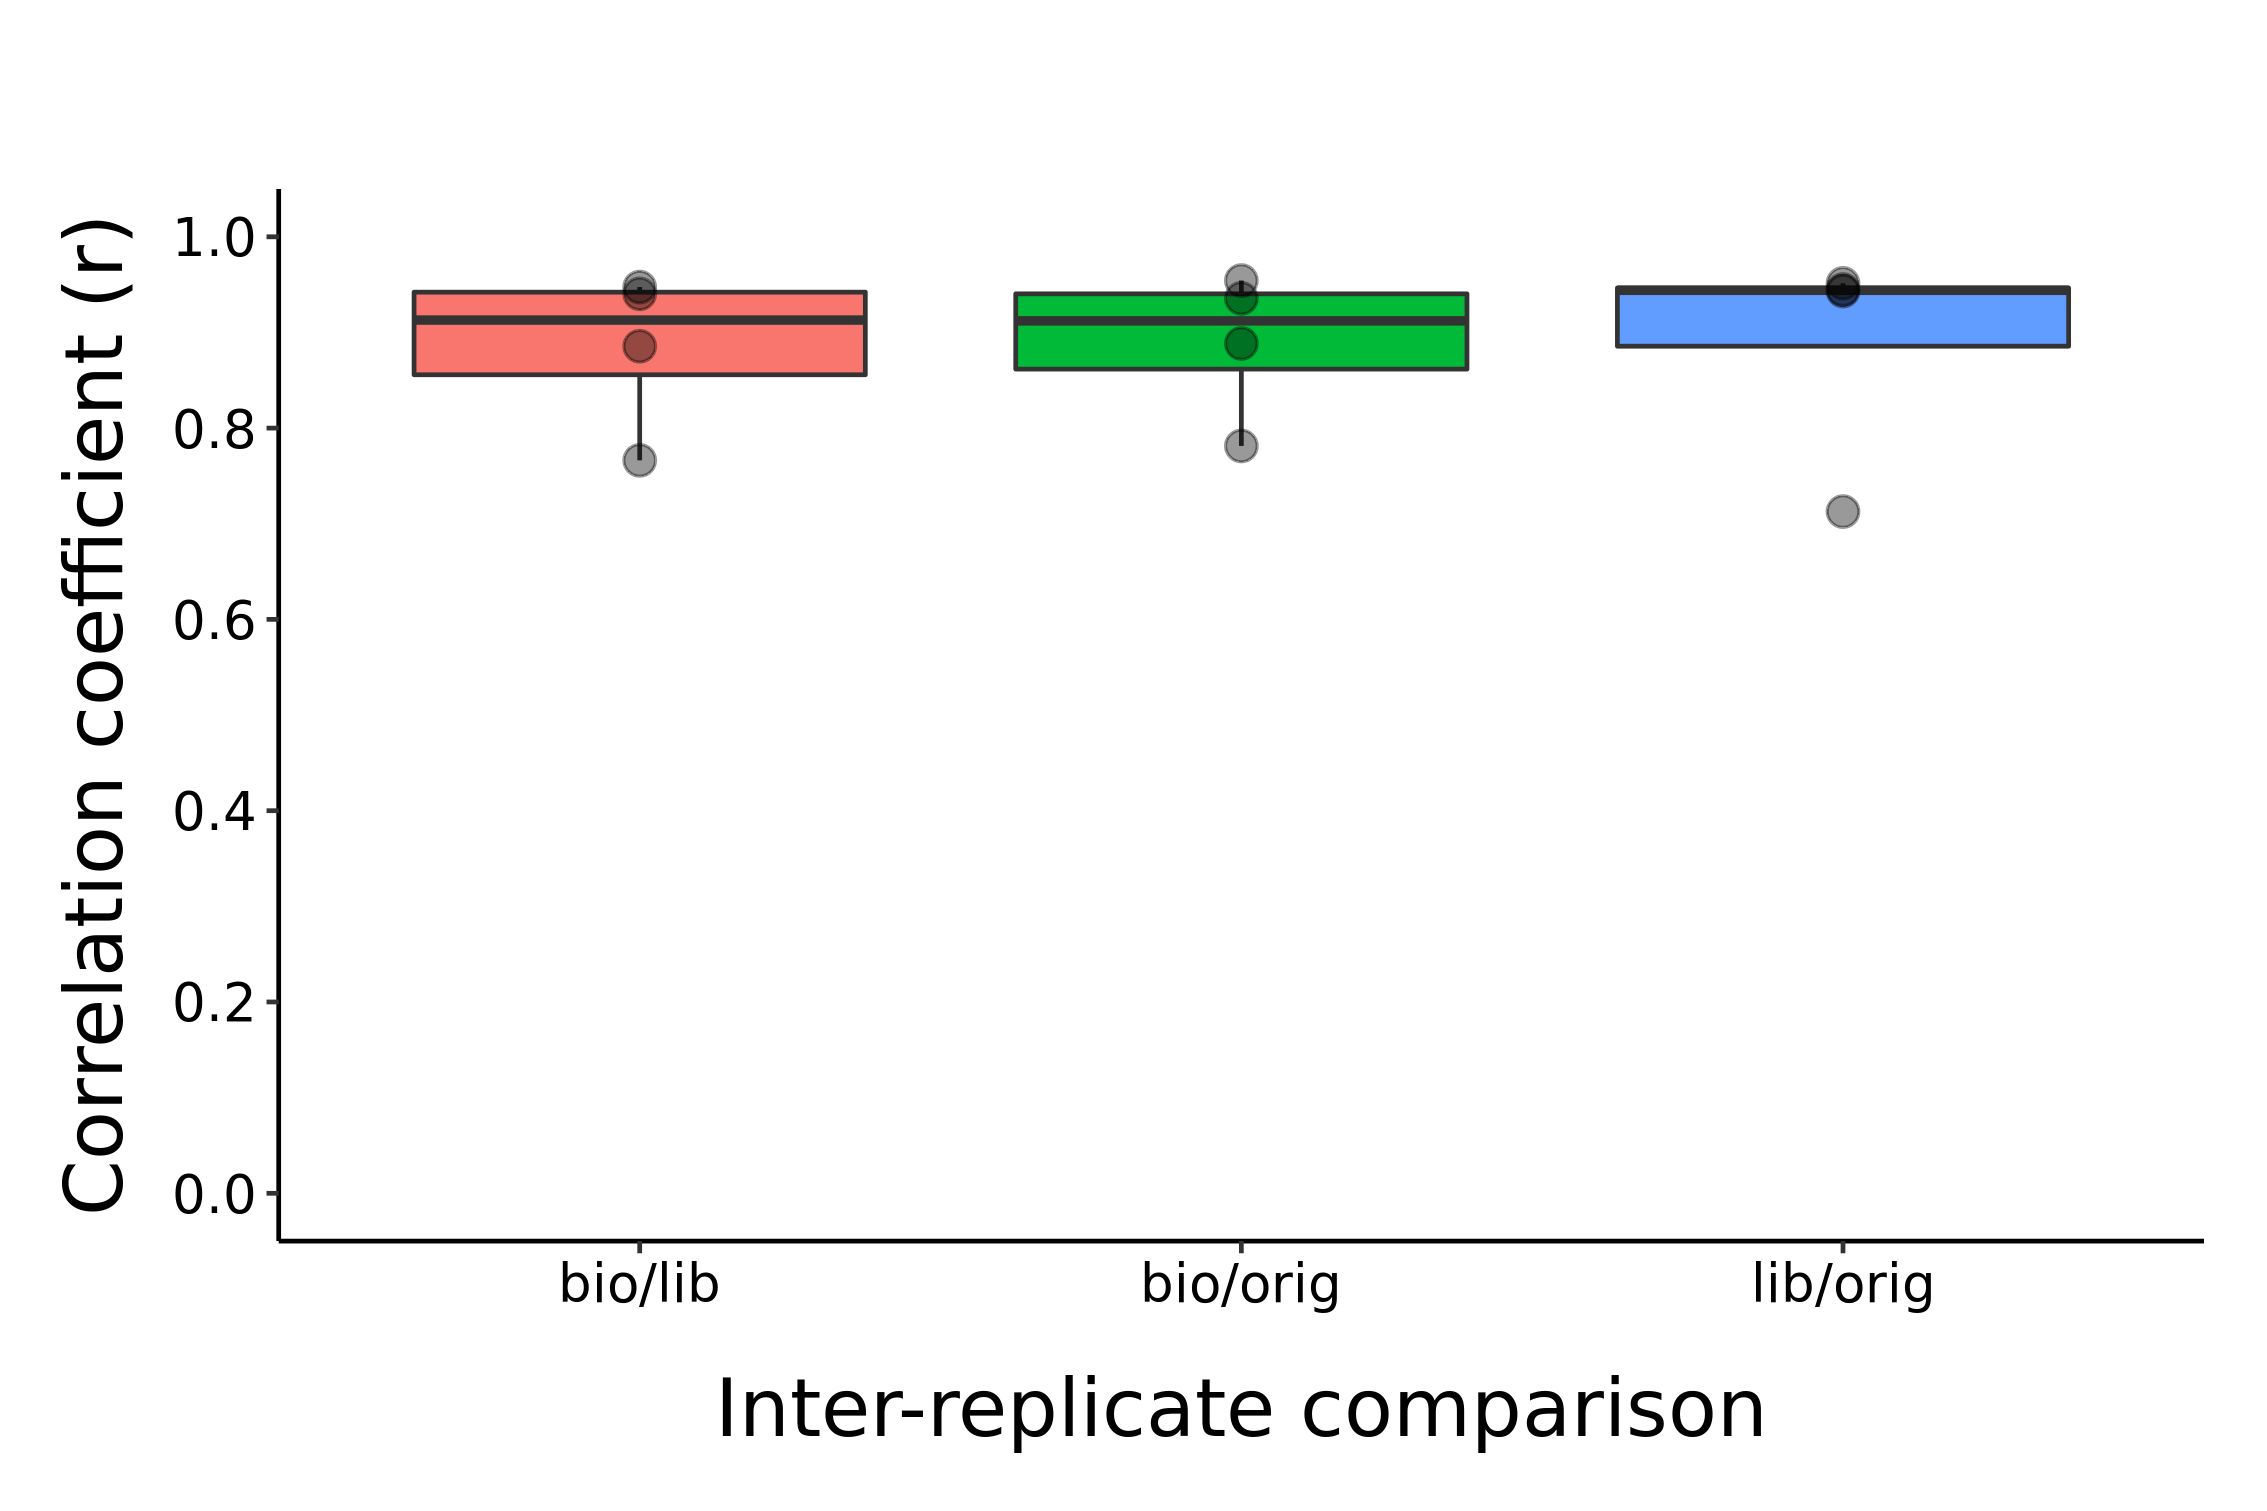
\includegraphics[width = 0.7\textwidth]{_Figures/png/pilot-clone-sizes-cor-boxplots}
\caption{Boxplots showing distribution of Pearson's product-moment correlation coefficients of clone sizes for each pair of replicates, as measured by the number of unique sequences per clone in each replicate. Clones absent in a given replicate were given a size of zero.}
% TODO: Add suitable overall figure title
\label{fig:igseq-pilot-clone-sizes-cor-boxplots}
\end{figure}

\begin{figure}
\centering
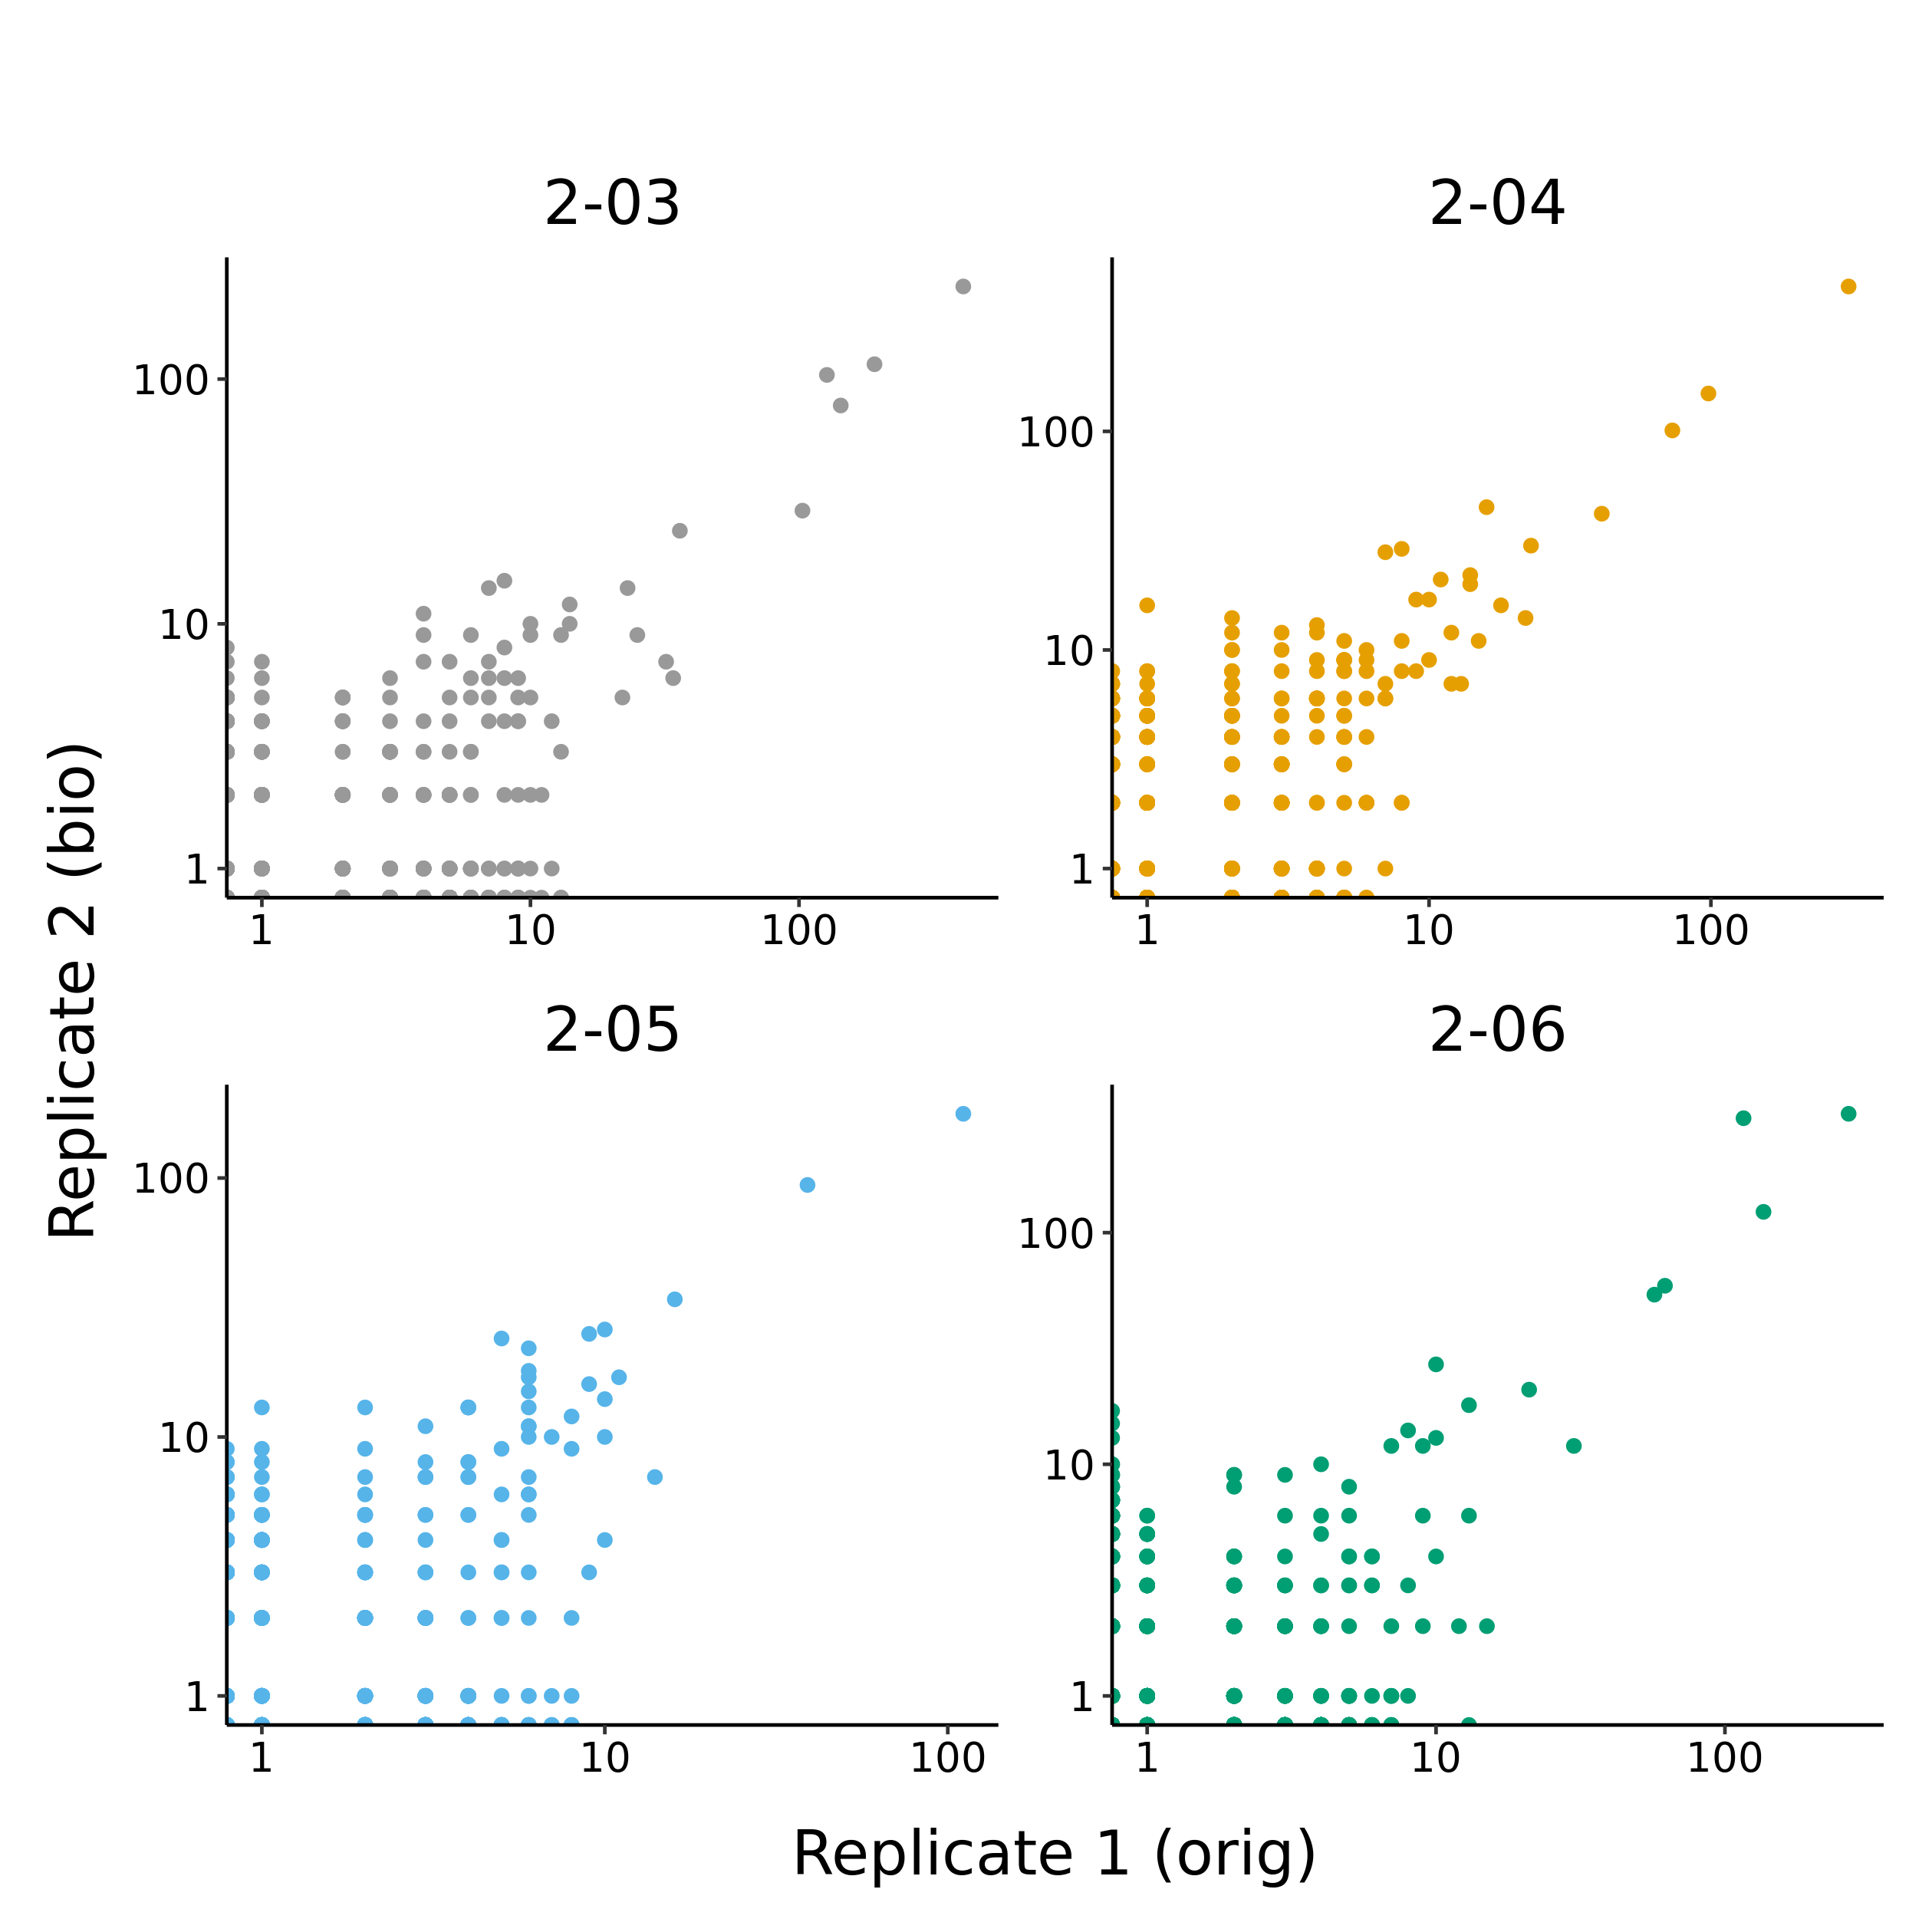
\includegraphics[width = 0.7\textwidth]{_Figures/png/pilot-clone-sizes-cor-scatter}
\caption{Scatter plots comparing clone sizes across biological replicates for each individual in the pilot dataset.}
% TODO: Add suitable overall figure title
\label{fig:igseq-pilot-clone-sizes-cor-scatter}
\end{figure}

% TODO: Needs a lead-in sentence. Why do you care?
One of the most strikingly reproducible findings of immune-repertoire-sequencing studies has been the approximately power-law distribution of the clonal repertoire, a phenomenon observed in both antibody and TCR repertoires across multiple different species \parencite{desponds2016fluctuating,mora2016diversity}. More precisely, the frequency of the $k$th largest clone in a repertoire dataset containing $N$ total clones can often be roughly predicted by a Zipf distribution \parencite{mora2010mentropy} of the form:

\begin{equation}
f(k | N, s) = \frac{x^{-s}}{H_{N,s}}
\end{equation}

\noindent for some exponent parameter $s > 0$, where $H_{N,s}$ is the $N$th generalised harmonic number of order $s$ (\Cref{sec:methods_comp_igdownstream_zipf}). This power-law distribution of clone sizes is inconsistent with clonal expansion under neutral selection and instead suggests that clone sizes evolve within a complex and fluctuating fitness landscape \parencite{desponds2016fluctuating}. % TODO: Read Desponds source for this
Before going on with more detailed investigation of the diversity structure of turquoise killifish antibody repertoires, it would be interesting to test whether the phenomenon of roughly Zipf-distributed clonal frequencies persists in this species as well.

\Cref{fig:igseq-pilot-clones-zipf-lines} shows the rank/frequency distributions of the clonal repertoires of the four individuals from the pilot dataset. From roughly the tenth-largest clone onwards, these distributions appear approximately linear on a log-log plot and can be reasonably approximated by a power-law distribution; % TODO: Stats for this?
however, the largest clones in each repertoire clearly deviate from this pattern, and are much larger than would be predicted by a power-law approximation. % I'm not sure how to interpret this; TODO: Ask AW about it?

\begin{figure}
\centering
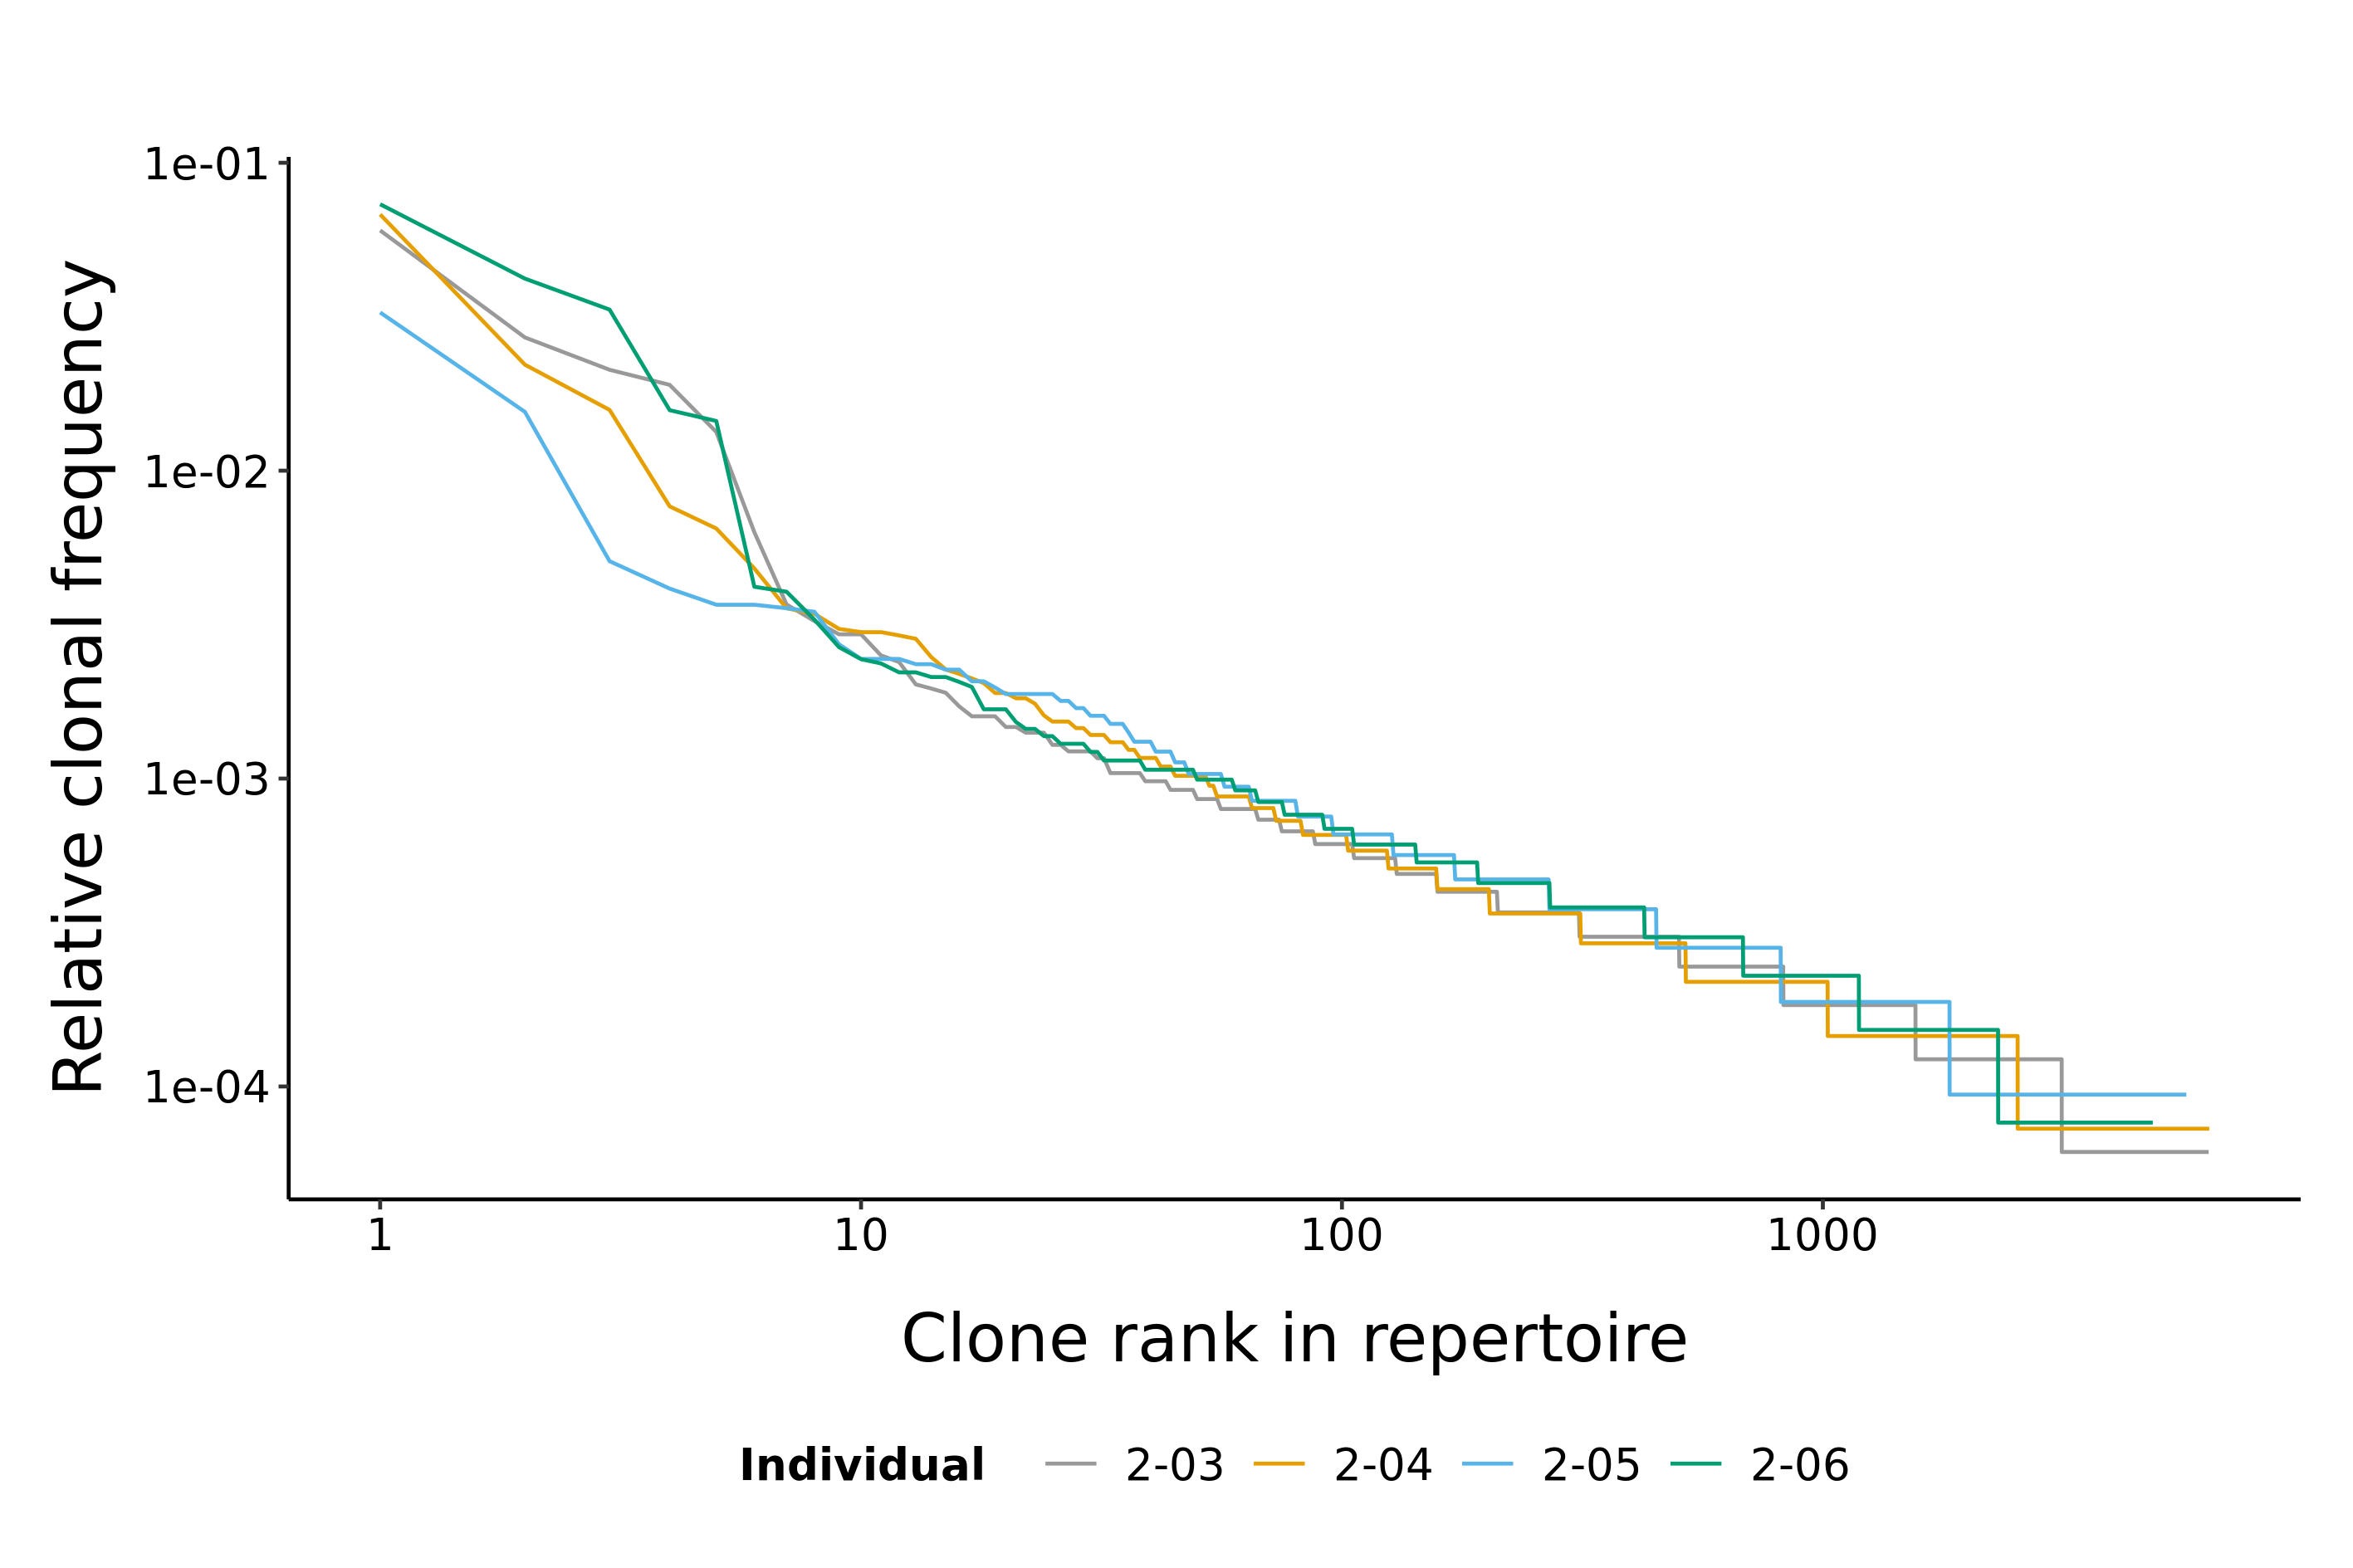
\includegraphics[width=0.8\textwidth]{_Figures/png/pilot-clones-zipf-lines}
\caption[Rank/frequency distributions of pilot clonal repertoires]{\textbf{Rank/frequency distributions of pilot clonal repertoires:} ...}
\label{fig:igseq-pilot-clones-zipf-lines}
\end{figure}

In order to fit power-law curves to these distributions, I performed simple maximum-likelihood estimation of the Zipf exponent for each individual repertoire in \program{R} (\Cref{sec:methods_comp_igdownstream_zipf}). When the five largest clones in each repertoire were excluded from the calculation, the resulting Zipf distributions (\Cref{fig:igseq-pilot-clones-zipf-fit}) provided a good approximation of the remaining points and were highly consistent across individuals, with exponents ranging from \embed{_Figures/txt/pilot-clones-zipf-exponent-min.txt} to \embed{_Figures/txt/pilot-clones-zipf-exponent-max.txt}. Conversely, when the largest clones are included, the resulting Zipf approximations follow the line of the remaining clones in several individuals much less accurately, and their exponents range more widely from \embed{_Figures/txt/pilot-clones-zipf-exponent-null-min.txt} to \embed{_Figures/txt/pilot-clones-zipf-exponent-null-max.txt}.

\begin{figure}
\centering
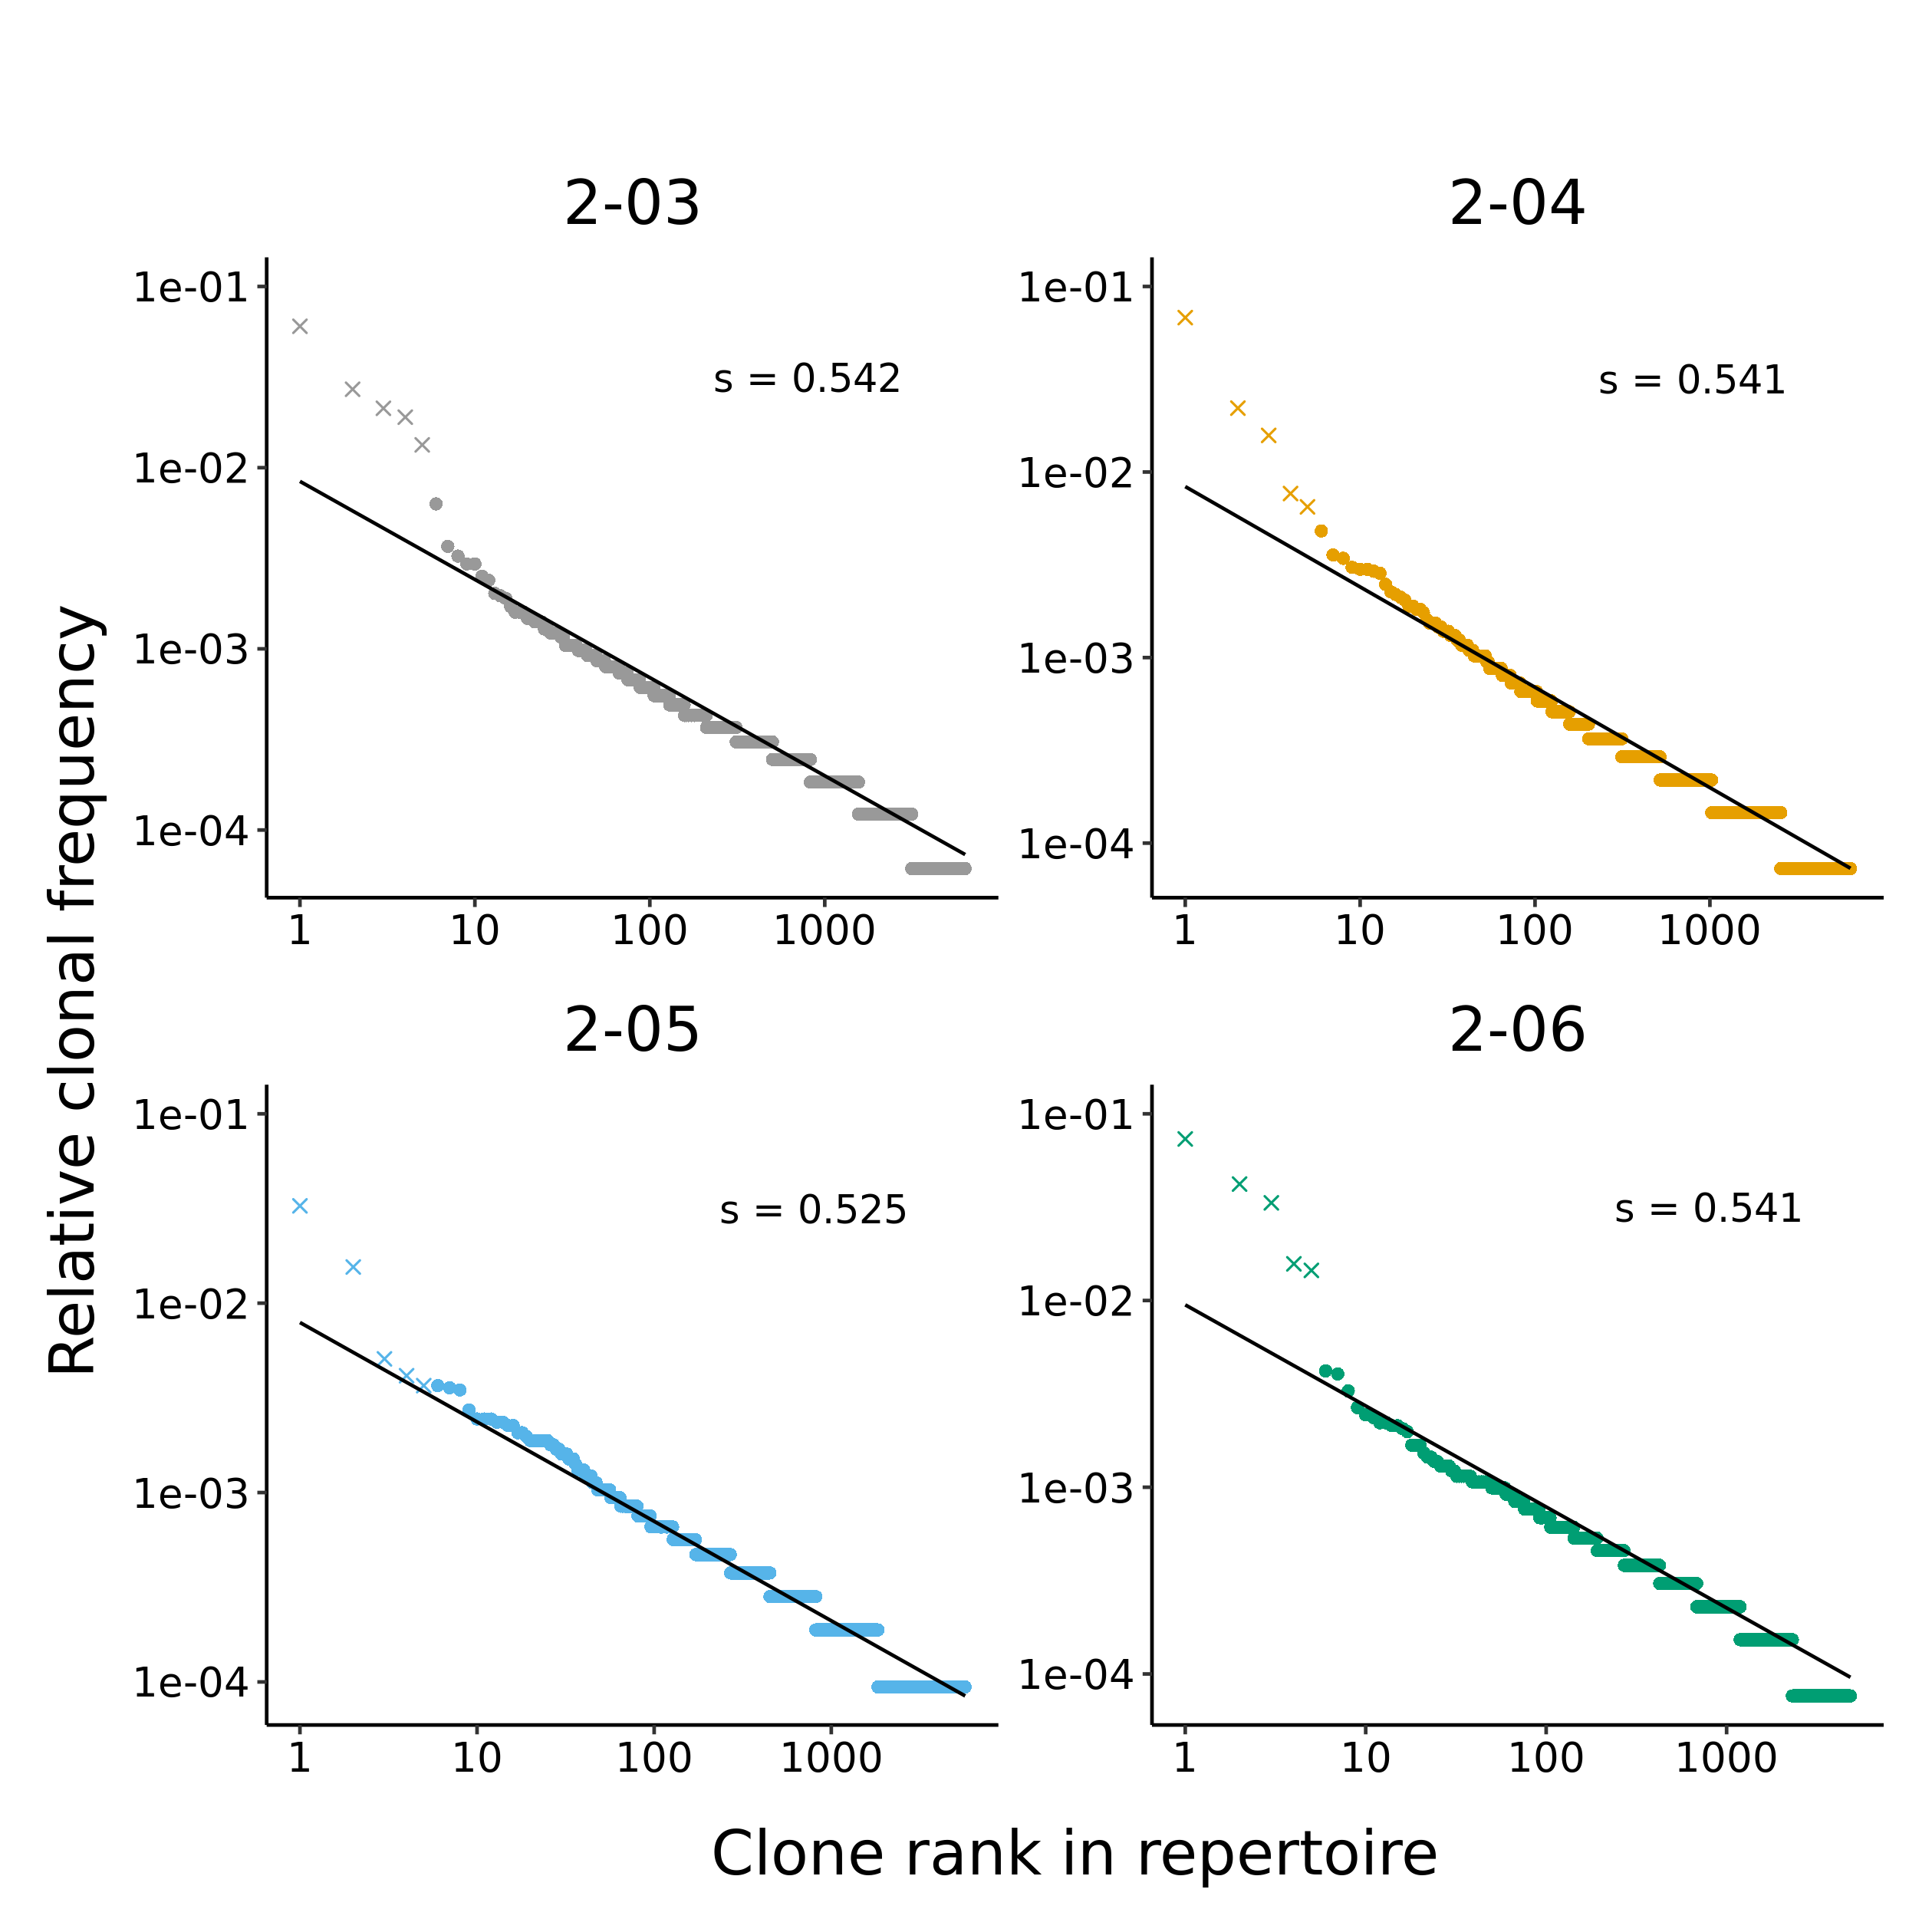
\includegraphics[width=0.8\textwidth]{_Figures/png/pilot-clones-zipf-fit}
\caption[...]{\textbf{...:} Log-log scatter plots of the rank/frequency distributions for each clonal repertoire in the pilot dataset, overlaid with a maximum-likelihood estimate of the underlying Zipf distribution when the five largest clones in each repertoire (plotted as crosses) are excluded.}
\label{fig:igseq-pilot-clones-zipf-fit}
\end{figure} % TODO: Add plot title

\begin{figure}
\centering
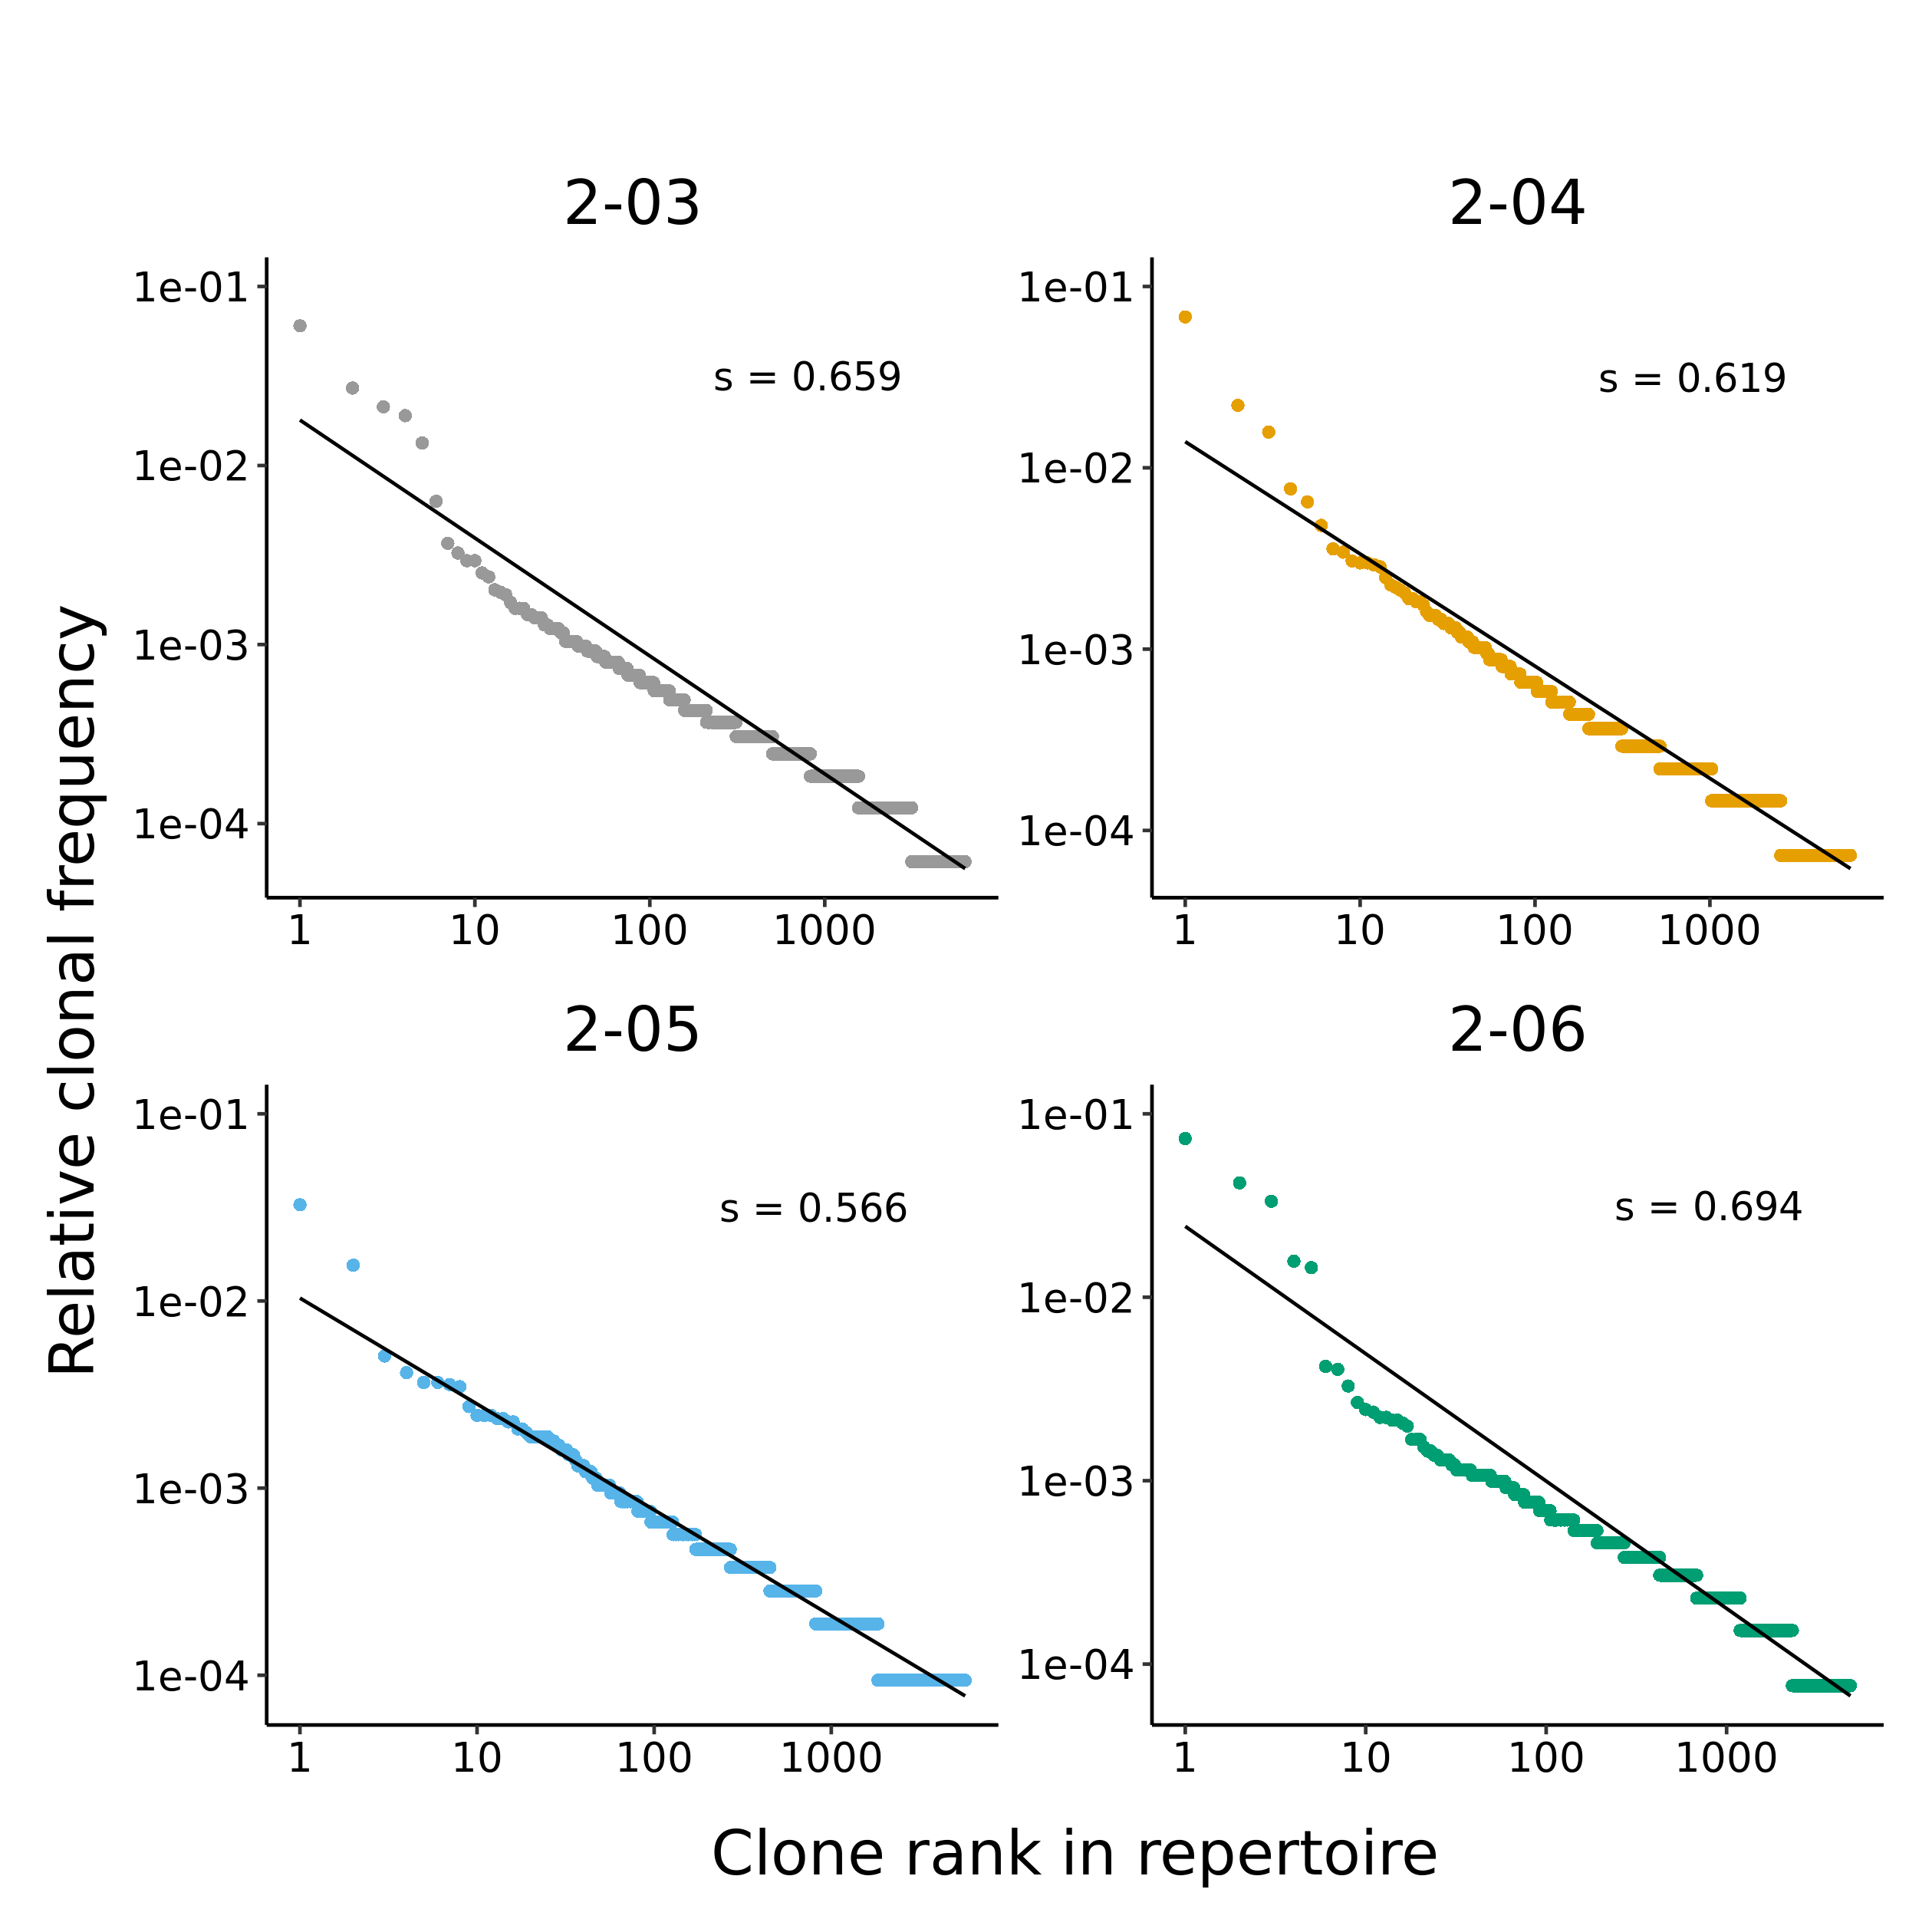
\includegraphics[width=0.8\textwidth]{_Figures/png/pilot-clones-zipf-fit-null}
\caption[...]{\textbf{...:} Log-log scatter plots of the rank/frequency distributions for each clonal repertoire in the pilot dataset, overlaid with a maximum-likelihood estimate of the underlying Zipf distribution when all clones (including the largest in each repertoire) are included in the inference process.}
\label{fig:igseq-pilot-clones-zipf-fit-null}
\end{figure} % TODO: Add plot title

...
% TODO: Final paragraph on Zipf data, interpreting and wrapping up
% TODO: Talk to AW / her lab members first

One quick and simple way to measure the extent to which a clonal repertoire is dominated by the largest clones is to measure the P20, the proportion of all unique sequences in the repertoire belonging to the 20 largest clones; in humans, for example, the P20 is typically a few percent in healthy individuals, but can reach up to 90\% in patients with B-cell malignancies \parencite{rosenfeld2018clonesize}. In the killifish pilot dataset, the P20 of the clonal repertoires ranges from \embed{_Figures/txt/pilot-clones-zipf-p20-obs-min.txt}\,\% to \embed{_Figures/txt/pilot-clones-zipf-p20-obs-max.txt}\,\%, much higher than that observed in healthy humans. These high P20 values are due to the highly expanded state of the largest few clones in each repertoire; when the expected clonal frequencies from the Zipf distributions fitted in \Cref{fig:igseq-pilot-clones-zipf-fit} are used instead of the actual values, the P20 values fall to between \embed{_Figures/txt/pilot-clones-zipf-p20-exp-min.txt}\,\% and \embed{_Figures/txt/pilot-clones-zipf-p20-exp-max.txt}\,\%.

\begin{figure}
\centering
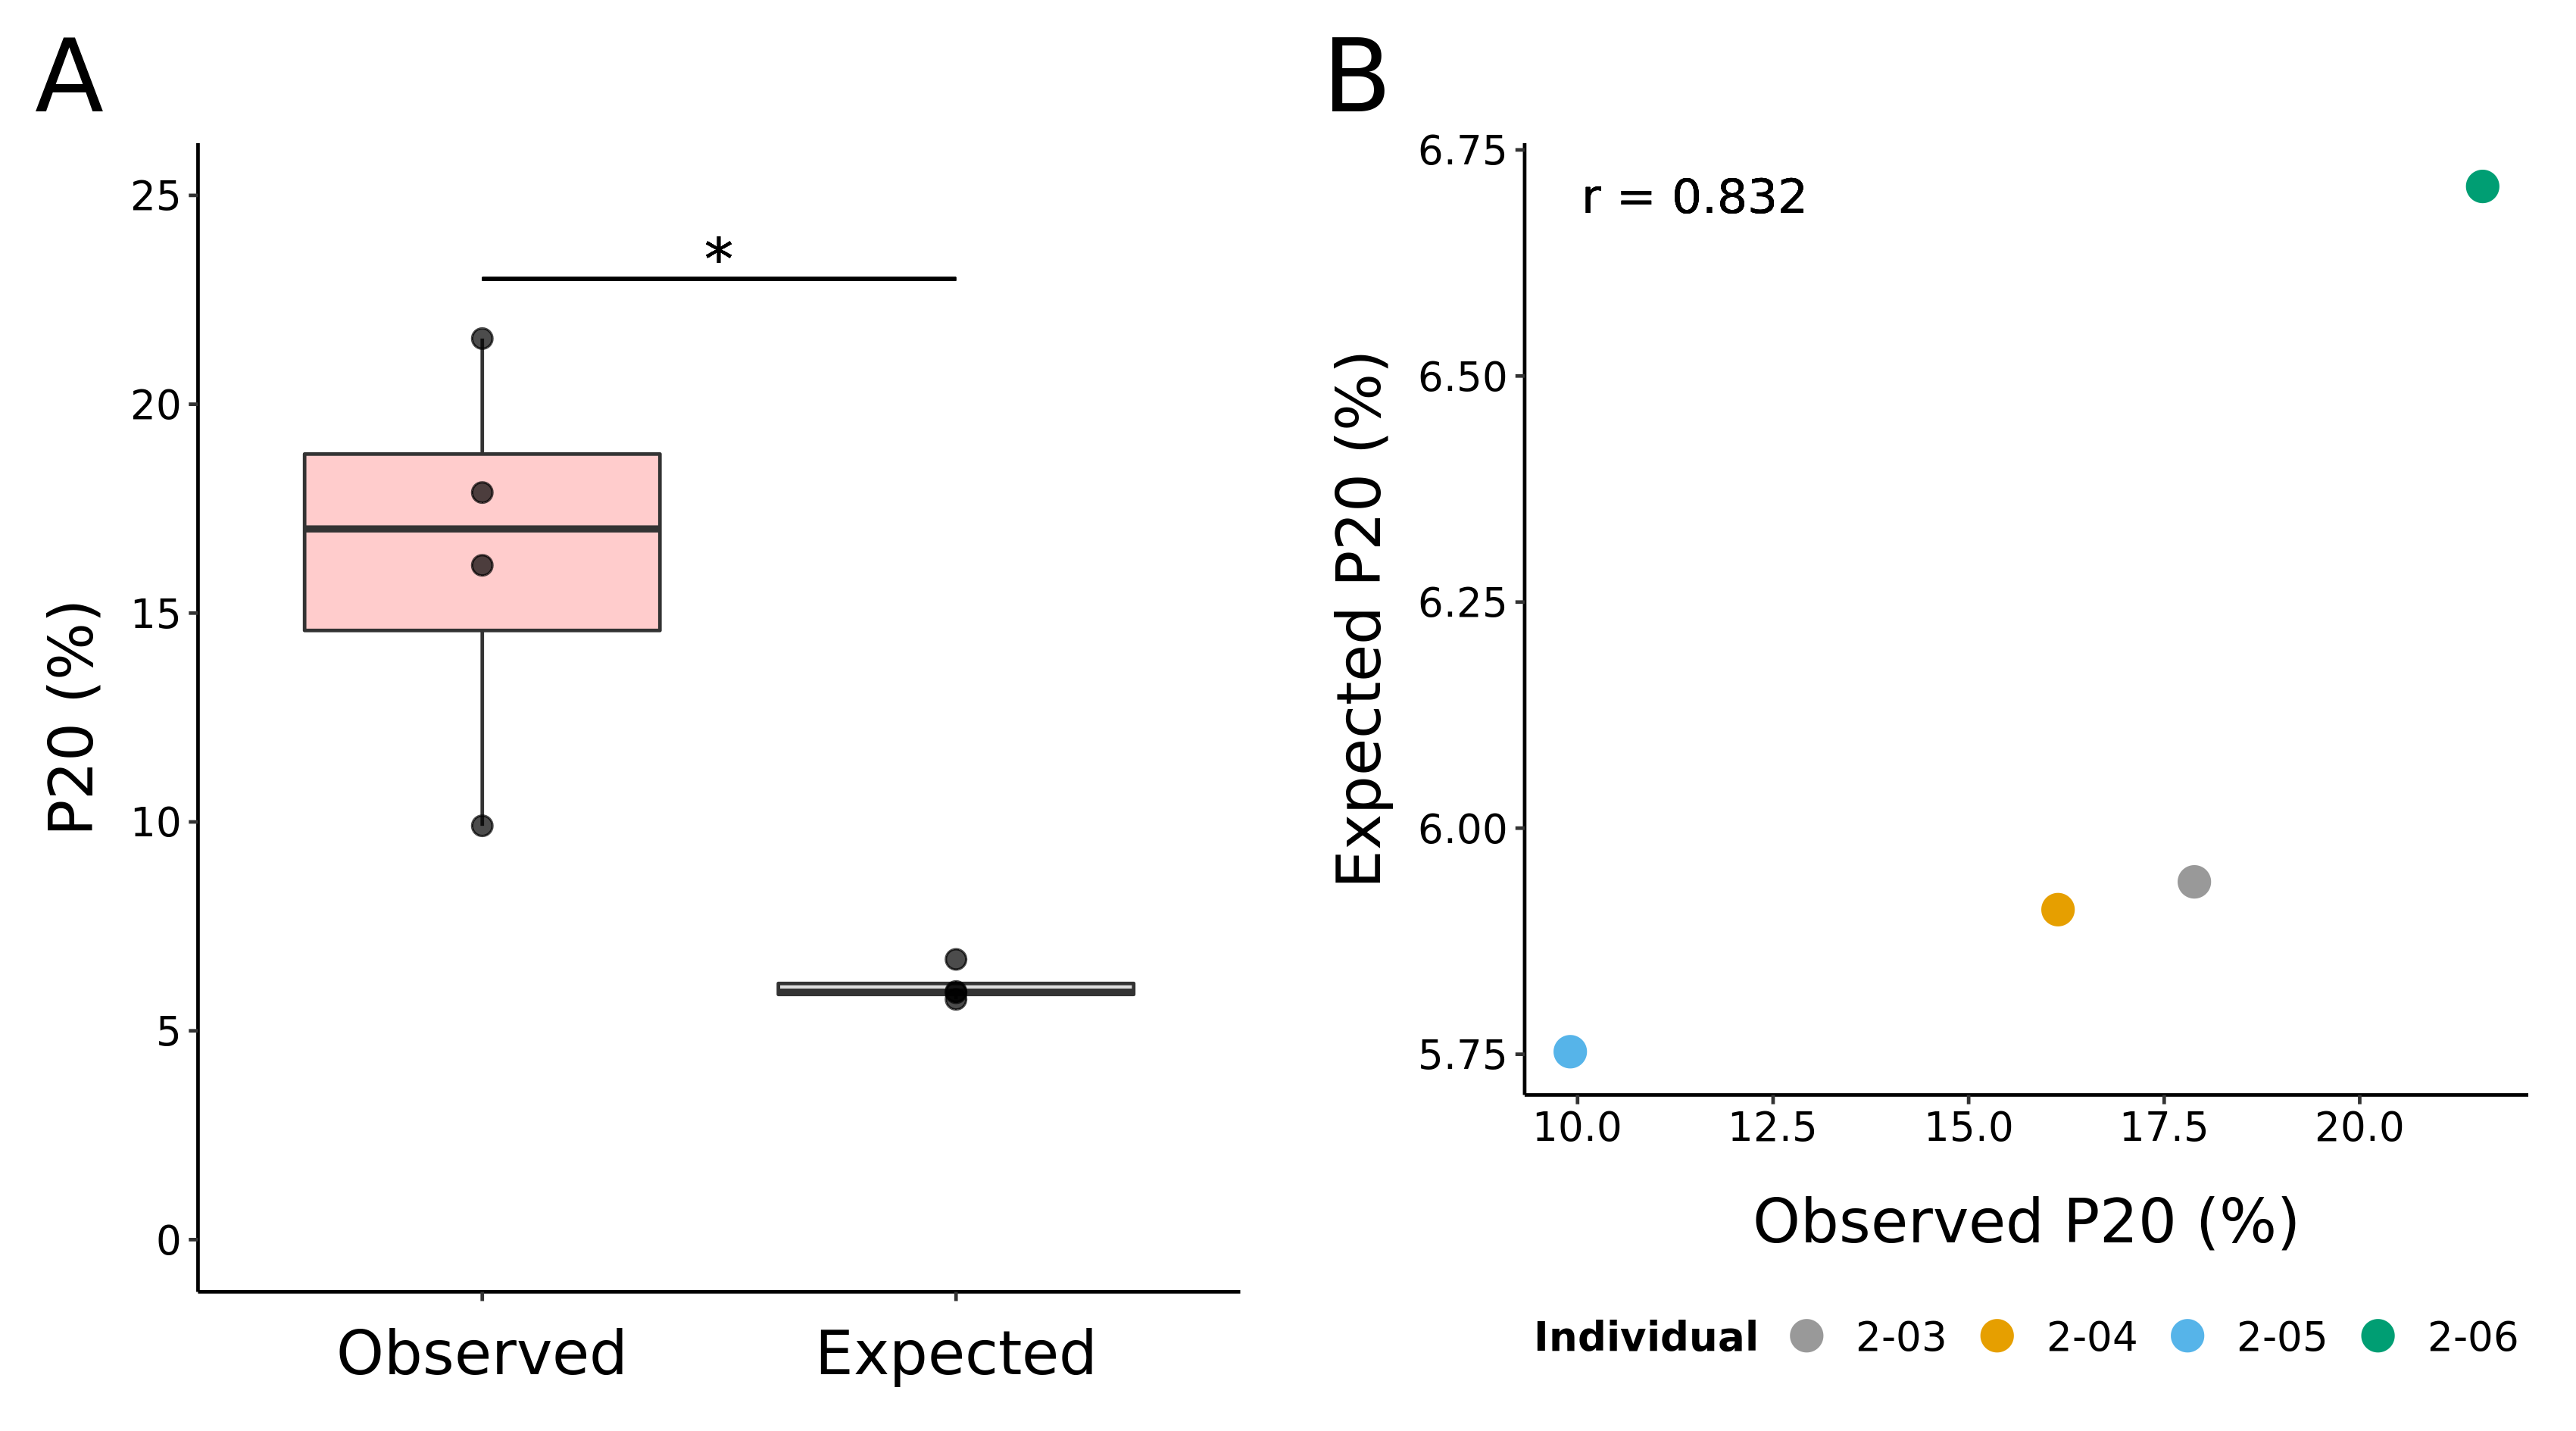
\includegraphics[width=0.8\textwidth]{_Figures/png/pilot-clones-zipf-p20-obs-exp}
\caption[Clonal P20 values in \Nfu pilot repertoires]{\textbf{Clonal P20 values in \Nfu pilot repertoires}: (A) Boxplots of observed and expected (from the Zipf distributions fitted in \Cref{fig:igseq-pilot-clones-zipf-fit}) P20 distributions of the clonal repertoires from the pilot \igseq dataset. Pairwise $p$-value computed using nonparametric Mann–Whitney U test ($*: 0.01 < p \leq 0.05;~**: 0.001 < p \leq 0.01;~***: p \leq 0.001$). (B) Scatter plot comparing observed \textit{versus} expected P20 for each individual, annotated with the correlation ($r$) between the two sets of P20 values.}
\label{fig:igseq-pilot-clones-zipf-p20}
\end{figure}

... . % TODO: Lead-in sentence here
Rosenfeld \textit{et al.} \parencite{rosenfeld2018clonesize} recommend evaluating clonal expansions on the basis of both the relative clonal frequency of the largest clones in the repertoire and the extent to which each such clone is larger than the next-largest clone, with recommended cutoffs for human data of 5\% for the former and threefold for the latter. In the pilot killifish dataset, clones exceeding 5\% of unique sequences in the repertoire occur in three out of four individuals (2-03, 2-04 and 2-06), while clones exceeding the size of the next-largest clone by at least threefold occur in a different three individuals (2-03, 2-05 and 2-06). However, only one individual, 2-04, exhibits a potentially medically-relevant clonal expansion by the standards of Rosenfeld \textit{et al.}; this clone (2-04\_8143) occupies 6.8\,\% of the repertoire and is roughly 3.1-fold larger than the next-largest clone, and is identified reproducibly as a clonal expansion in both the pooled dataset (\Cref{fig:igseq-pilot-clones-expansions-rep}) and each of the separate replicates (\Cref{fig:igseq-pilot-clones-expansions-rep}) from individual 3-04.
... . % TODO: Interpretation: what does this mean for 8-week-old killifish repertoires? Why does it matter? Can we rely on the frequencies from Rosenfeld?

\begin{figure}
\centering
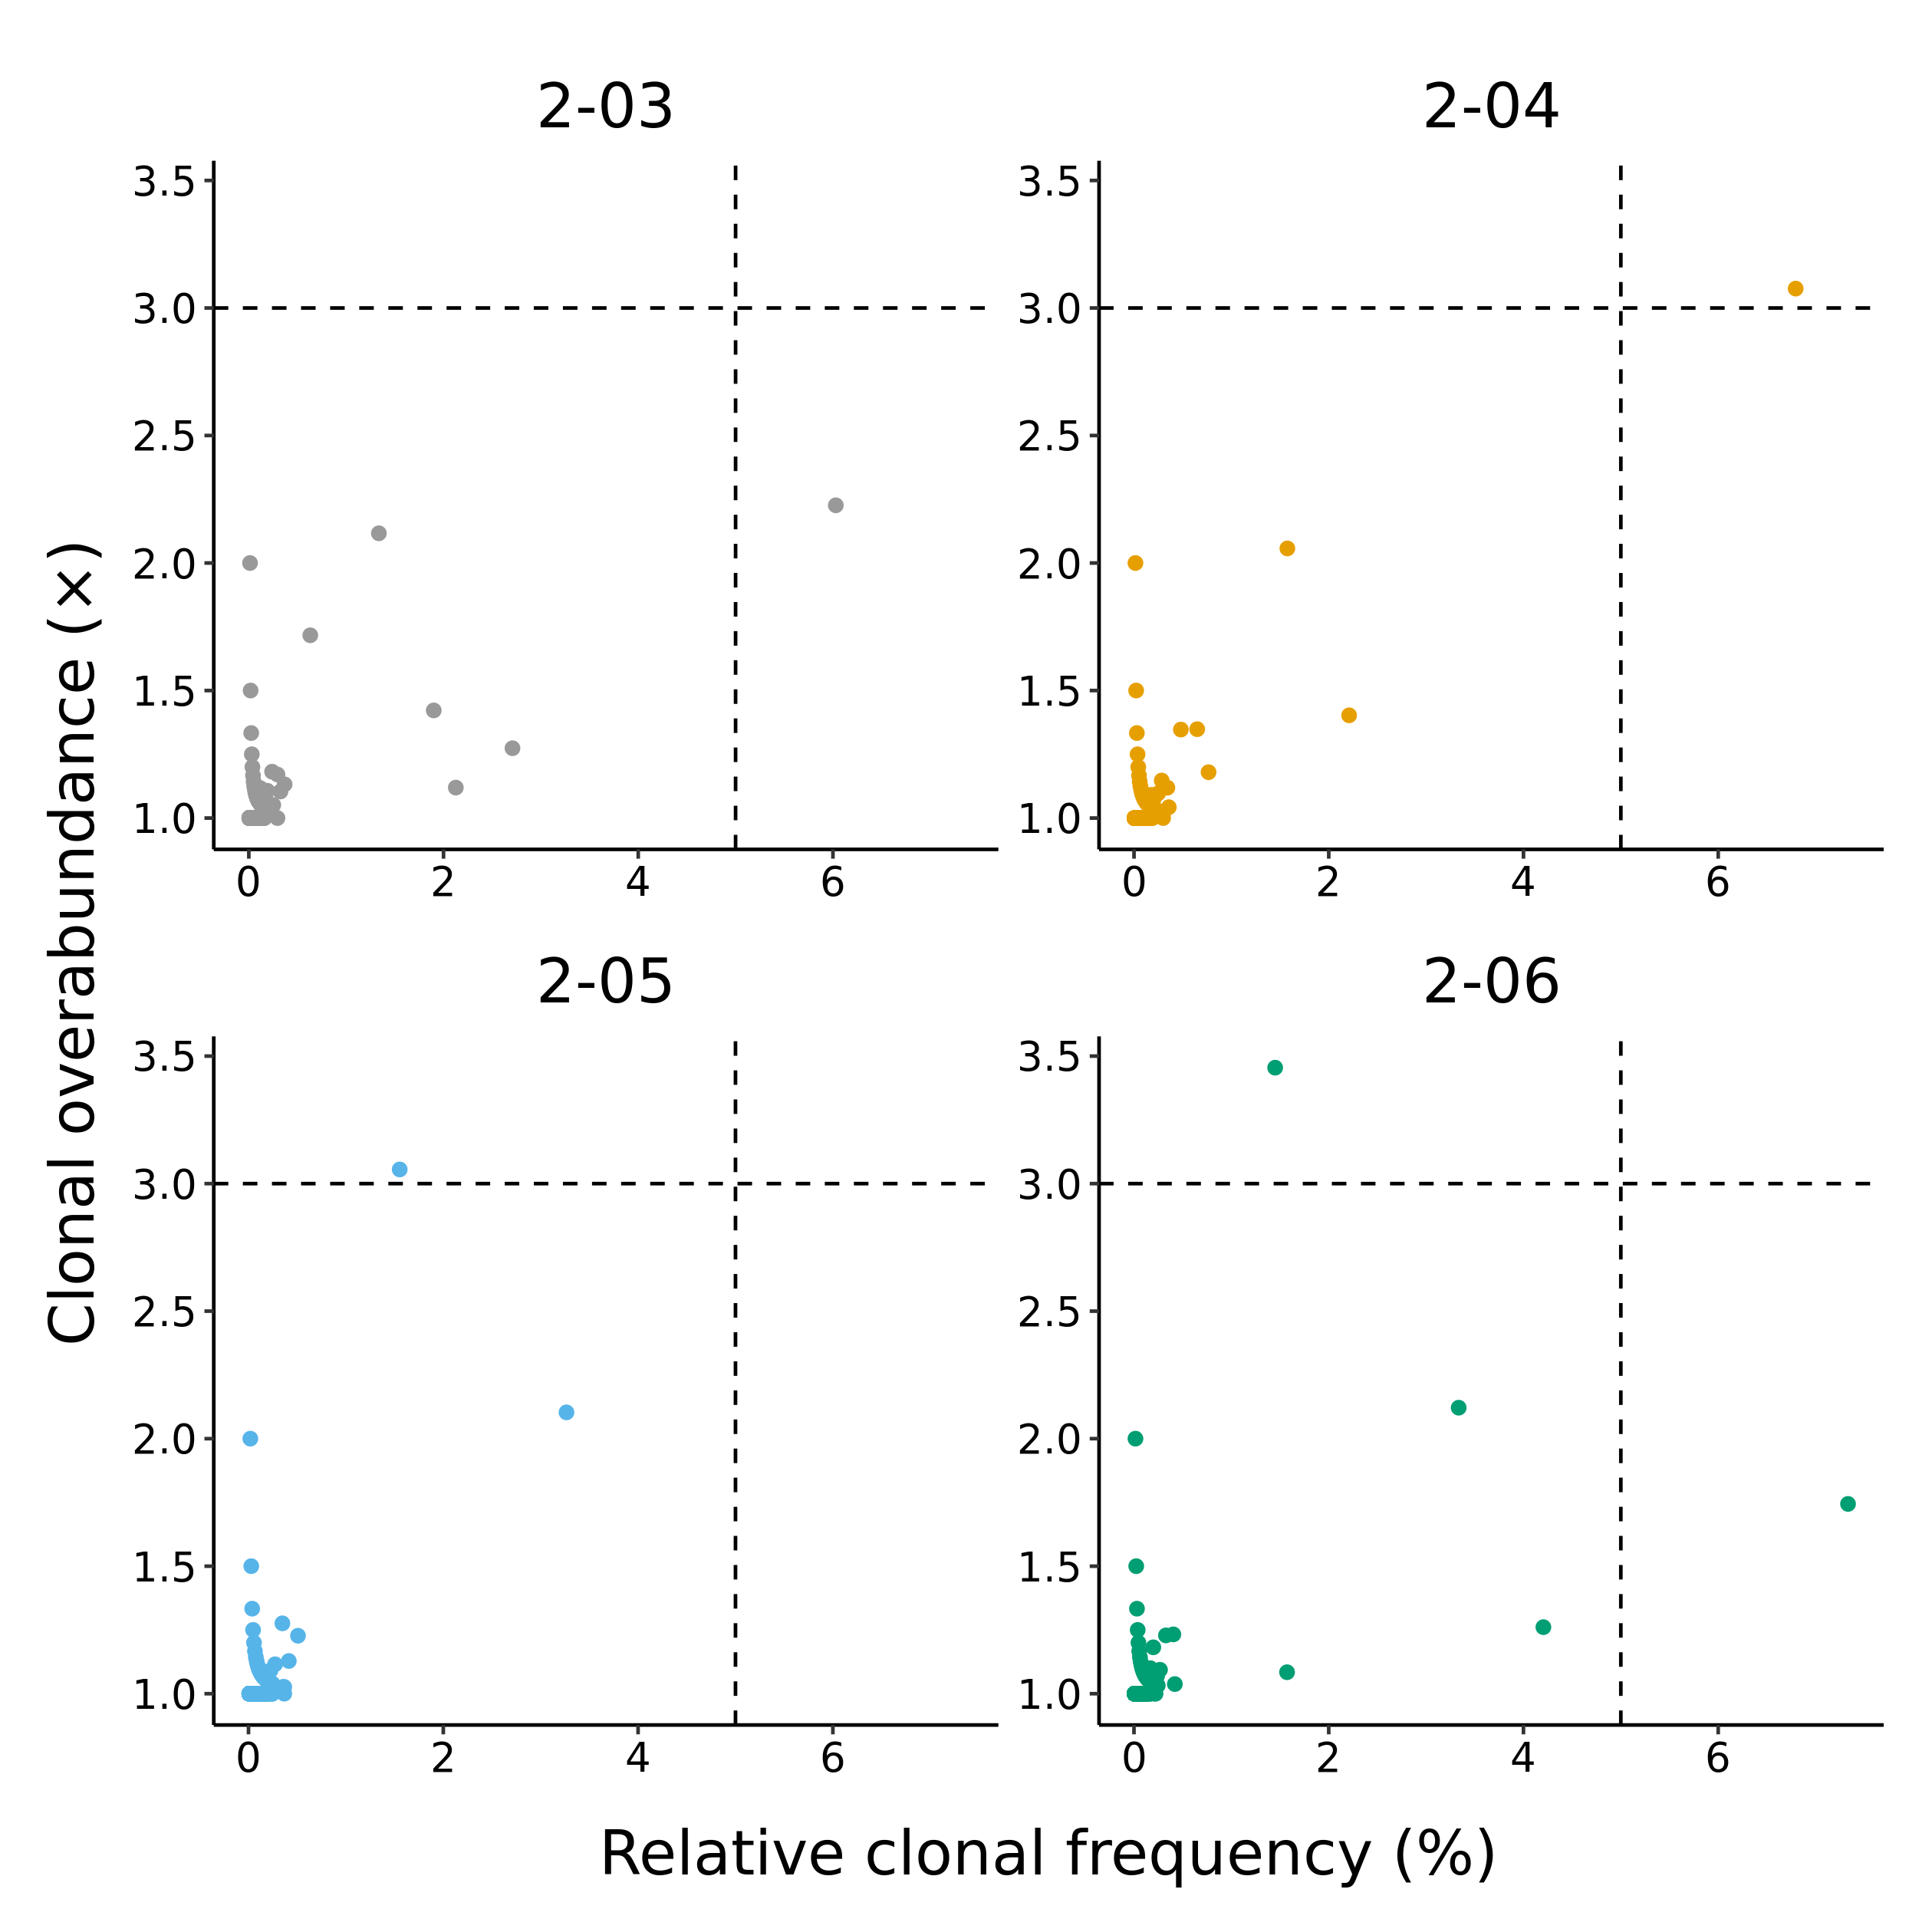
\includegraphics[width=0.8\textwidth]{_Figures/png/pilot-clones-expansions}
\caption[Clonal expansions in \Nfu pilot repertoires]{\textbf{Clonal expansions in \Nfu pilot repertoires}: Scatter plots of clonal abundance for each individual in the pilot \igseq dataset, measured in terms of the proportion of unique sequences in the repertoire ($x$-axis) and the abundance relative to the next-largest clone ($y$-axis). Thresholds for identifying clonal expansions (5\,\% and 3-fold for the $x$- and $y$-axis, respectively) suggested by Rosenfeld \textit{et al.} \parencite{rosenfeld2018clonesize}.}
\label{fig:igseq-pilot-clones-expansions}
\end{figure}

Having investigated the clonal abundance distribution and various measures of clonal expansion, we now come to the question of the \textit{diversity} of the killifish clonal repertoire. As discussed in detail in \Cref{app:diversity}, the diversity of a population can be interpreted -- and measured -- in multiple ways, with different measures laying different amounts of weight on the richness (number of species) and evenness (relative distribution of species) of that population and reporting the results in different ways. In order to visualise the diversity of killifish clonal repertoires across a wide range of diversity orders (...) % TODO: Find a way to explain diversity orders concisely
simultaneously and on a common scale, Hill diversity spectra % Citation needed
can be used. These ... . % TODO: Concise explanation
A more detailed explanation, including the underlying equations, can be found in \Cref{app:diversity}.

\Cref{fig:igseq-pilot-clone-diversity} shows the diversity of clone sizes in each individual in the pilot dataset, as measured using Hill diversity spectra across each individual's three replicates (\Cref{fig:igseq-pilot-design}). \Cref{fig:igseq-pilot-clone-diversity-alpha} gives the alpha diversity, or average \textit{within-replicate} diversity, while \Cref{fig:igseq-pilot-clone-diversity-beta} shows the beta-diversity, or variation in clone-size distribution \textit{between} replicates (\Cref{app:diversity}). In both cases, each curve represents a single individual and gives the corresponding diversity measure at a range of different diversity orders; roughly speaking, higher diversity orders place proportionately more weight on common over rare species (i.e. clones) when calculating diversity, with zero-order diversity being equivalent to simple species richness (\Cref{app:diversity}). As beta-diversity (unlike alpha-diversity) is sensitive to the number of sub-populations being compared, it has been rescaled here such that 0 represents the minimum possible beta-diversity at each order and 1 represents the maximum (\Cref{app:diversity}).
% TODO: Explain rescaling in diversity appendix
% TODO: More precise references to appendix subsections

\begin{figure}
\centering
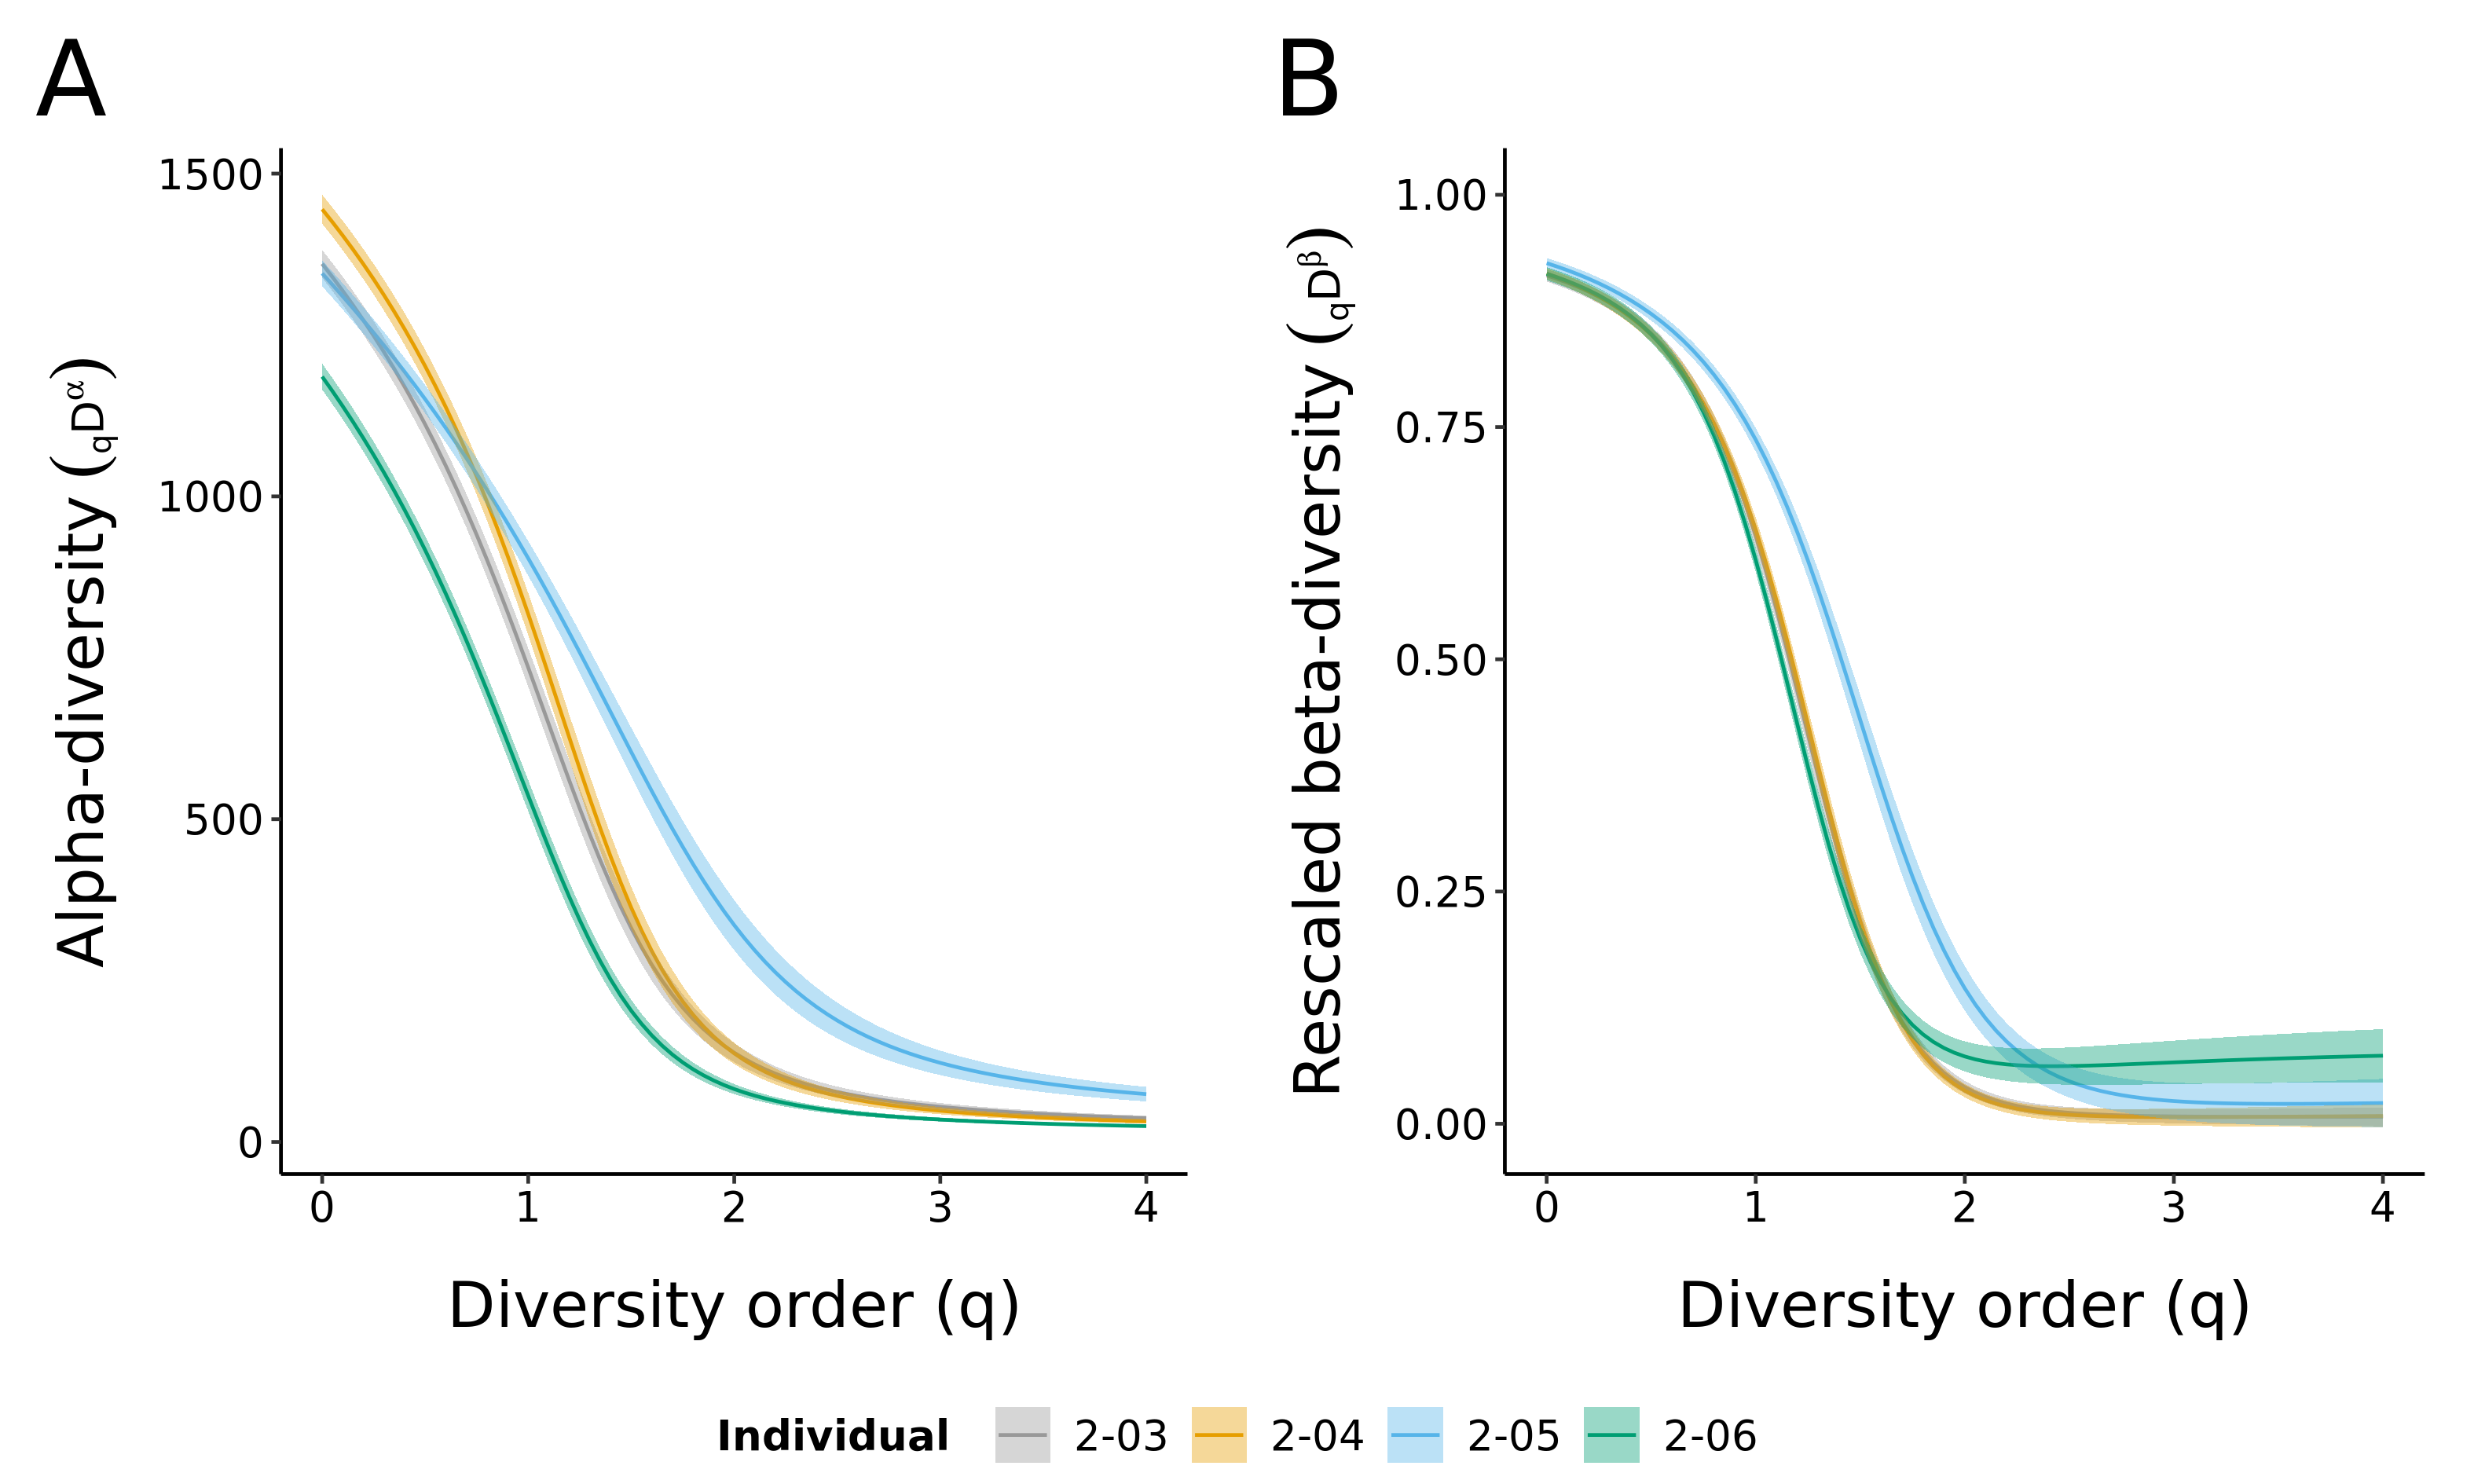
\includegraphics[width = 0.9\textwidth]{_Figures/png/pilot-clone-diversity}
\begin{subfigure}{0em}
\phantomsubcaption{}
\label{fig:igseq-pilot-clone-diversity-alpha}
\end{subfigure}
\begin{subfigure}{0em}
\phantomsubcaption{}
\label{fig:igseq-pilot-clone-diversity-beta}
\end{subfigure}
\caption{\textbf{Clonal diversity spectra for pilot dataset:} Hill diversity spectra of clone sizes (as measured by number of unique sequences per clone) over replicates for each individual in the pilot dataset. (A) Alpha-diversity across replicates; (B) Beta-diversity across replicates, rescaled to between 0 (minimum) and 1 (maximum) for each individual. Shaded regions in both subfigures represent 95\,\% confidence intervals, estimated using bootstrapping.} % TODO: Parametric or nonparametric?
\label{fig:igseq-pilot-clone-diversity}
\end{figure}

The results from the alpha-diversity spectrum (\Cref{fig:igseq-pilot-clone-diversity-alpha}) suggest there may be significant differences in diversity between individuals in middle-aged killifish: in particular, individual 2-06 appears to be less diverse than the other individuals across the whole range of diversity orders (suggesting that its clonal repertoire both contains fewer clones overall and is more uneven in its clone sizes) while individual 2-05 appears to be more diverse at higher diversity orders (suggesting that its clonal repertoire is of similar richness to the other individuals, but more even). This would accord with previous measures of P20 and Zipf exponent in these repertoires (\Cref{fig:igseq-pilot-clones-zipf-fit-null,fig:igseq-pilot-clones-zipf-p20}), both of which suggest that the clonal repertoire of 2-06 is substantially more expanded than the other individuals in the dataset, and that of 2-05 less so.

However, when comparing alpha-diversities across sample groups, by-eye comparisons of apparent diversities is of course not sufficient for concluding that a significant difference in diversity exists. Ideally, the entire shape of the diversity spectrum would be compared between groups to test for a significant difference in distribution; however, the unusual and non-parametric nature of the Hill spectrum makes such a holistic comparison difficult, and established tests for such a difference do not yet exist to my knowledge. However, it is possible to use established statistical methods to test for a difference in Hill diversity at one or more specific diversity orders, and so to obtain a partial overview of significant differences for particular aspects of each group's diversity profile. 

To that end, I computed the clonal diversity spectra separately for each replicate in the pilot dataset (\Cref{fig:igseq-pilot-clone-diversity-solo-spectra}), and extracted the distribution of diversity values obtained for each individual at each of six diversity orders (0, 1, 1.5, 2, 3 and 4). I compared these distributions pairwise using Mann-Whitney $U$ nonparametric tests, as well as performing a Kruskal-Wallis nonparametric analysis-of-variance test for an effect of source individual on repertoire diversity. Neither of these tests returned a significant result for any of the diversity orders tested (\Cref{fig:igseq-pilot-clone-diversity-solo-box}). From the data available, therefore, it is not possible to conclude that clonal repertoires differ significantly between individuals in middle-aged adult male turquoise killifish, though given the relatively low Kruskal-Wallis $p$-values obtained at higher diversity orders (\Cref{fig:igseq-pilot-clone-diversity-solo-box}) it is possible such a difference would be observed if more replicates per individual were available.
% TODO: Citations for MWU, KWT

\begin{figure}
\centering
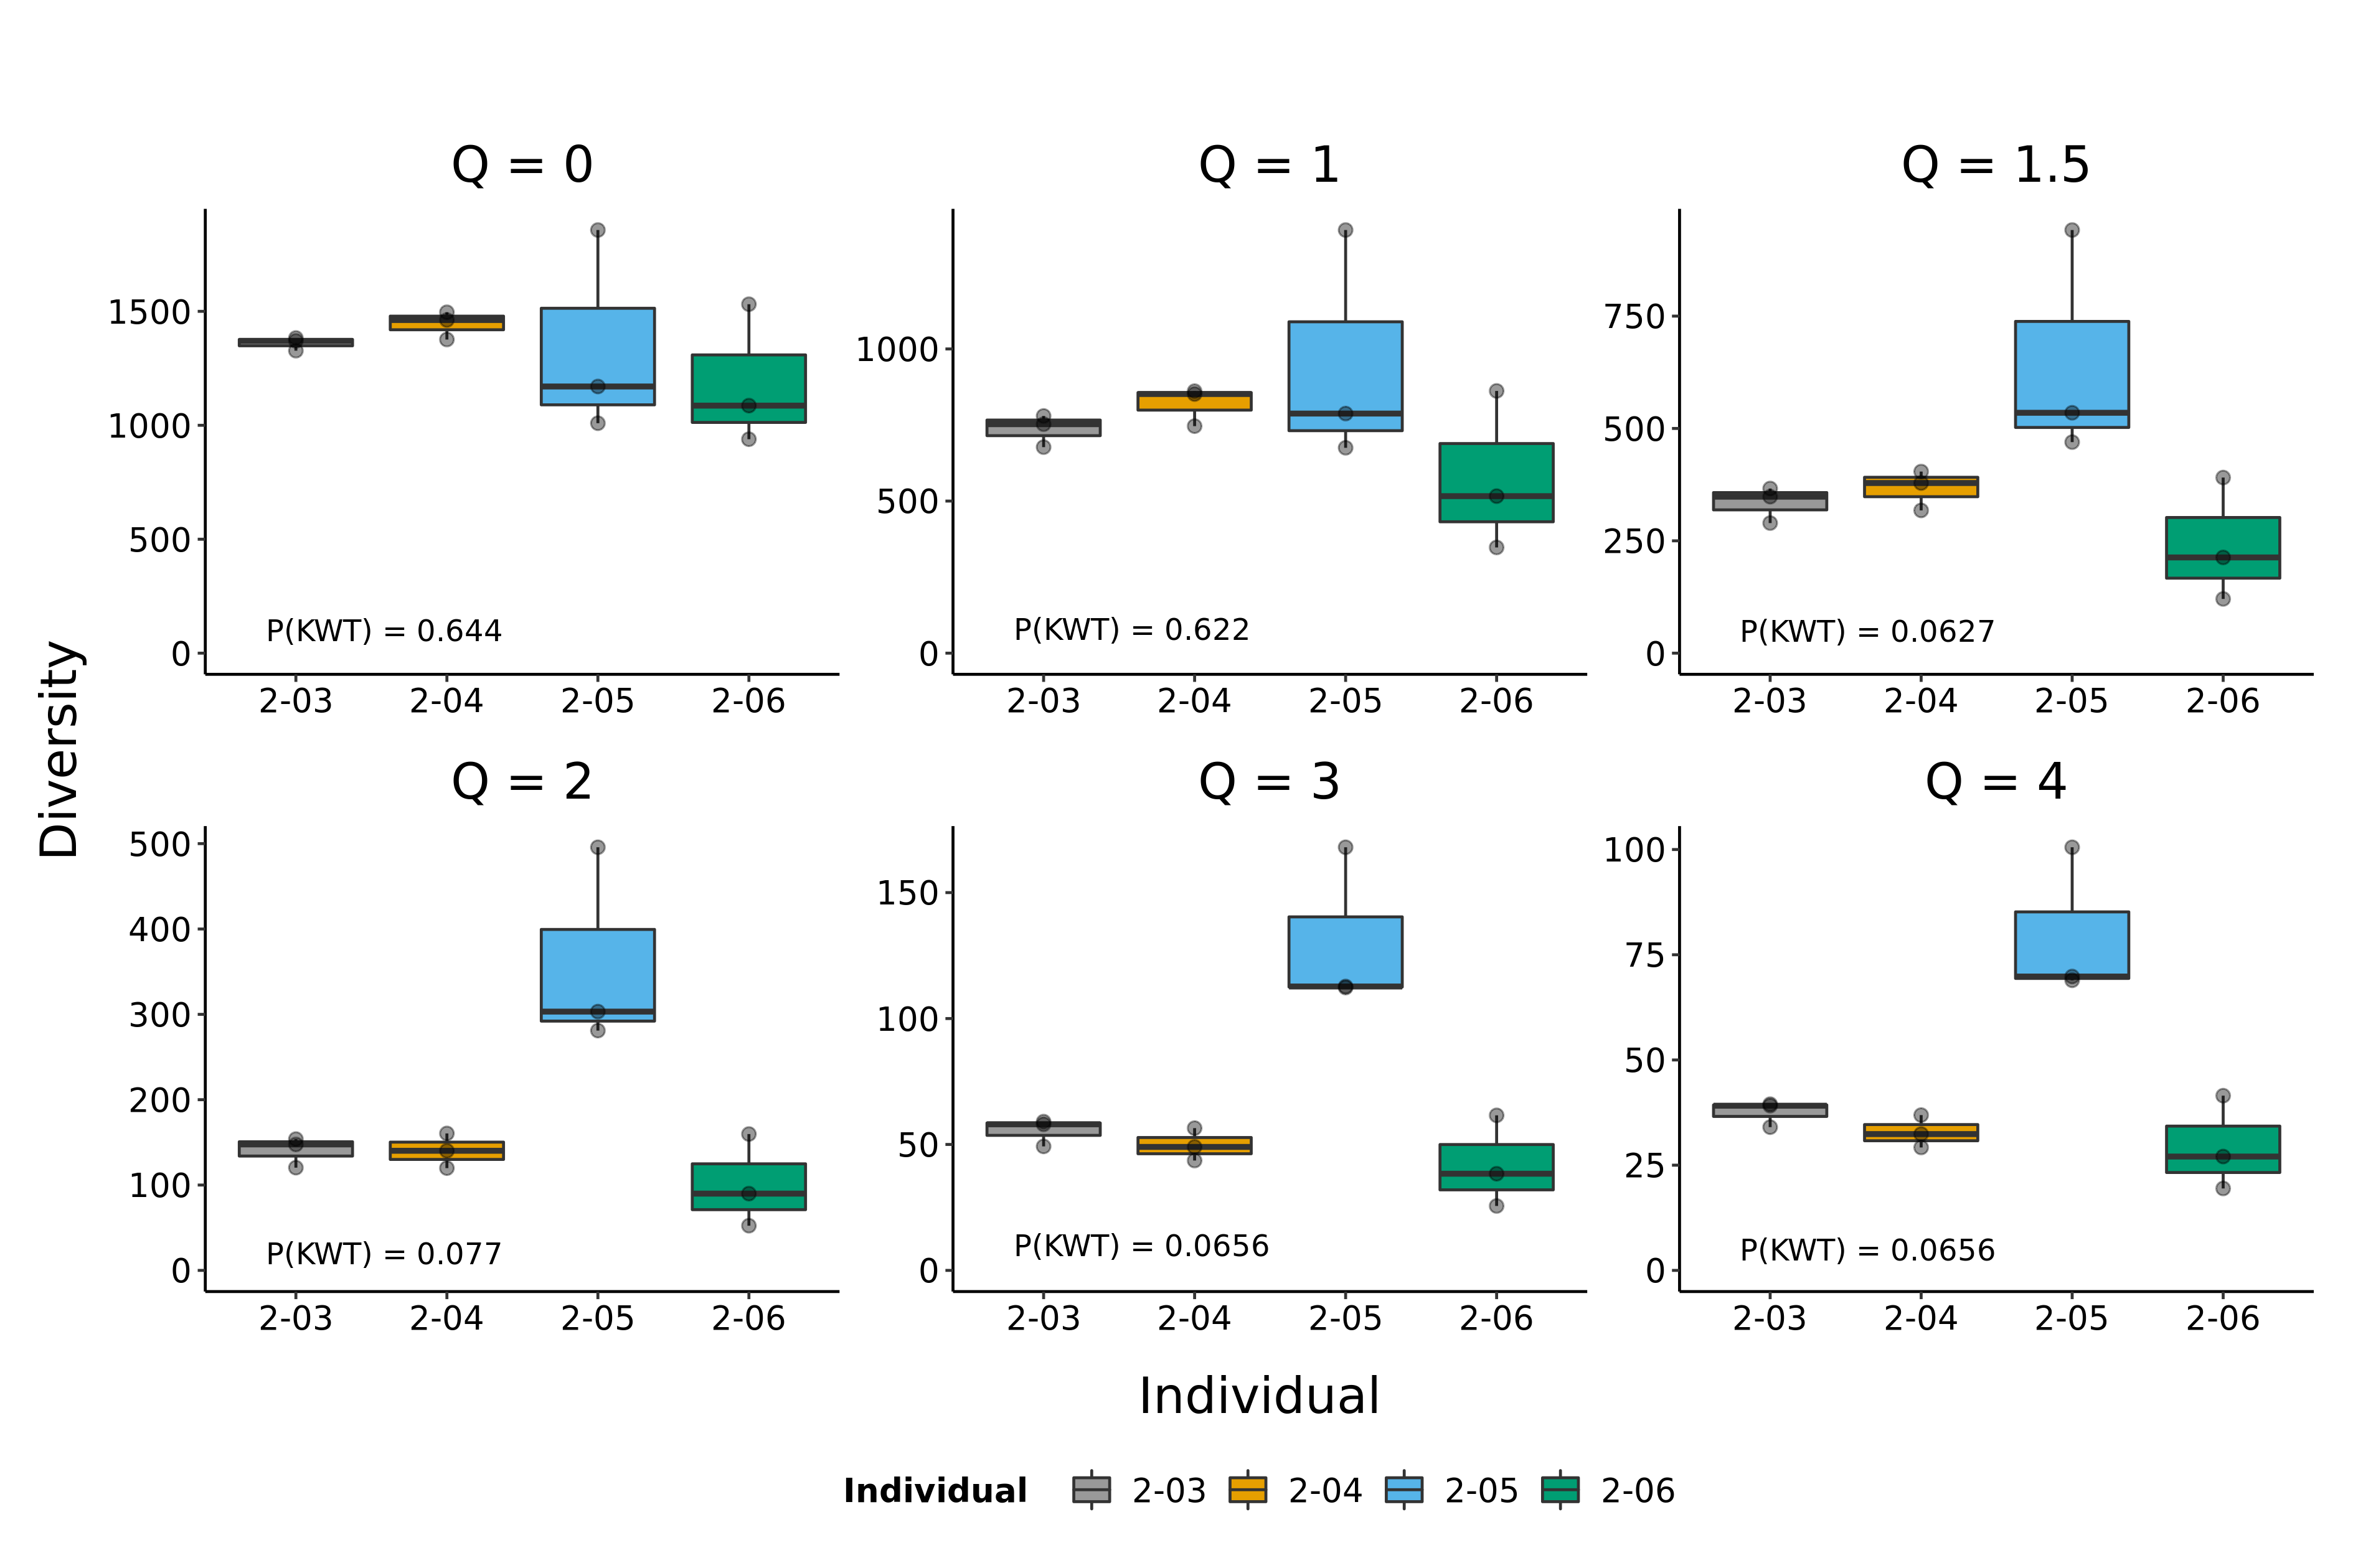
\includegraphics[width = 0.8\textwidth]{_Figures/png/pilot-clone-diversity-solo-box}
\caption{Boxplots of Hill diversity values for the clonal repertoires of replicates from each individual in the \igseq pilot dataset at a sample of diversity orders. Pairwise $p$-values are computed using nonparametric Mann–Whitney U tests ($*: 0.01 < p \leq 0.05;~**: 0.001 < p \leq 0.01;~***: p \leq 0.001$). Annotated $p$-values ($P(KWT)$) indicates the statistical significance of the estimated individual effect on diversity at each order under a Kruskal-Wallis test.} % TODO: Figure title
\label{fig:igseq-pilot-clone-diversity-solo-box}
\end{figure}

Unlike alpha-diversity, the beta-diversity spectrum of a population does not necessarily decline monotonically with increasing diversity order; nevertheless, in \Cref{fig:igseq-pilot-clone-diversity-beta} the between-replicate beta-diversity is much higher at low diversity orders (where it approaches the maximum) than at higher ones (where it is close to the minimum). This indicates that replicates from the same individual have very different clonal content when all clones are included, but become increasingly similar as more and more weight is put on the largest clones in each replicate. This result is highly consistent with the findings in \Cref{fig:igseq-pilot-clone-sizes} that each repertoire contains a small number of large clones (which are shared reproducibly between replicates) and a much larger number of much smaller clones (which are not); the difference in patterns of cross-replicate reproducibility between small and large clones observed in \Cref{fig:igseq-pilot-clone-sizes-reps} gives rise to the patterns of beta-diversity observed in \Cref{fig:igseq-pilot-clone-diversity-beta}.

Finally, given the apparent correspondence between a high P20 or fitted Zipf exponent and low effective diversity as measured using Hill spectra, I investigated to what extent these measures, which are substantially quicker and easier to compute than full diversity spectra, act as good proxies for properly-estimated Hill diversity. To that end, I fitted Zipf distributions separately to the clonal repertoires of each replicate in the dataset (both including all clones and excluding the five largest in each repertoire, as above) as well as computing the P20 for these repertoires. I then computed Pearson product-moment correlation coefficients % TODO: Citation needed
at each diversity order, enabling correlation spectra to be plotted for each of the three potential proxy metrics. I did this both for the correlation between per-replicate proxy metrics and per-replicate repertoire diversity (\Cref{fig:igseq-pilot-clone-diversity-metrics-cor-rep}) and between per-individual averaged metrics and per-individual alpha diversity (\Cref{fig:igseq-pilot-clone-diversity-metrics-cor-alpha}). 

At the per-replicate level, the filtered Zipf exponent performed fairly poorly at all diversity orders, while the all-clones Zipf exponent and P20 both performed relatively poorly at very low orders but correlated well with higher-order diversity measures ($q \geq 1$), with P20 consistently outperforming either Zipf exponent as a predictor of Hill diversity; best of all is \embed{_Figures/txt/pilot-clone-diversity-metrics-cor-rep-best-metric.txt} at $q=\embed{_Figures/txt/pilot-clone-diversity-metrics-cor-rep-best-q.txt}$, with a correlation coefficient of \embed{_Figures/txt/pilot-clone-diversity-metrics-cor-rep-best-r.txt}. When comparing averaged metrics with average (alpha) per-individual diversity, the pattern for the all-clones Zipf exponent and P20 is broadly similar, albeit reaching much lower correlation values: at $q=\embed{_Figures/txt/pilot-clone-diversity-metrics-cor-avg-best-q.txt}$, the average \embed{_Figures/txt/pilot-clone-diversity-metrics-cor-avg-best-metric.txt} approaches a near-perfect correlation of \embed{_Figures/txt/pilot-clone-diversity-metrics-cor-avg-best-r.txt}. Conversely, the filtered Zipf exponent behaves very differently in the average case compared to the per-replicate case, with even worse prediction at very low diversity orders but improving greatly at higher orders, to the point where, from $q=\embed{_Figures/txt/pilot-clone-diversity-metrics-cor-avg-cross-q.txt}$ upwards, it actually correlates better with Hill diversity than either P20 nor the all-clones Zipf exponent, with an optimum correlation of \embed{_Figures/txt/pilot-clone-diversity-metrics-cor-avg-sfilter-best-r.txt} at $q=\embed{_Figures/txt/pilot-clone-diversity-metrics-cor-avg-sfilter-best-q.txt}$.
% TODO: Can I explain this, or is it "surprisingly, however"?

It therefore appears that the diversity of the clonal repertoire can be predicted well by P20 and Zipf proxy metrics across most of the range of diversity orders, the exception being low orders substantially less than 1. These low orders are primarily (or exclusively, in the case of $q=0$) measures of clonal richness which neglect clone size when computing diversity; as P20 and Zipf exponents are both measures of the extent to which the repertoire is dominated by the largest clones, it is perhaps unsurprising that they are less well-equipped to predict the lower-order diversity of the clonal repertoire. % TODO: Citation needed?
... % TODO: Discuss meaning and usefulness of these correlation results

In conclusion, therefore, adult turquoise killifish express diverse clonal B-cell repertoires, with each fish containing several thousand detected clones. As in other species, this repertoire comprises a few very large expanded clones % TODO: How many unique sequences in very large clones?
and a much larger number of very small clones, the latter of which are highly vulnerable to undersampling. ... % TODO: Finish overview paragraph

\begin{figure}
\centering
\begin{subfigure}{0em}
\phantomsubcaption{}
\label{fig:igseq-pilot-clone-diversity-metrics-cor-rep}
\end{subfigure}
\begin{subfigure}{0em}
\phantomsubcaption{}
\label{fig:igseq-pilot-clone-diversity-metrics-cor-alpha}
\end{subfigure}
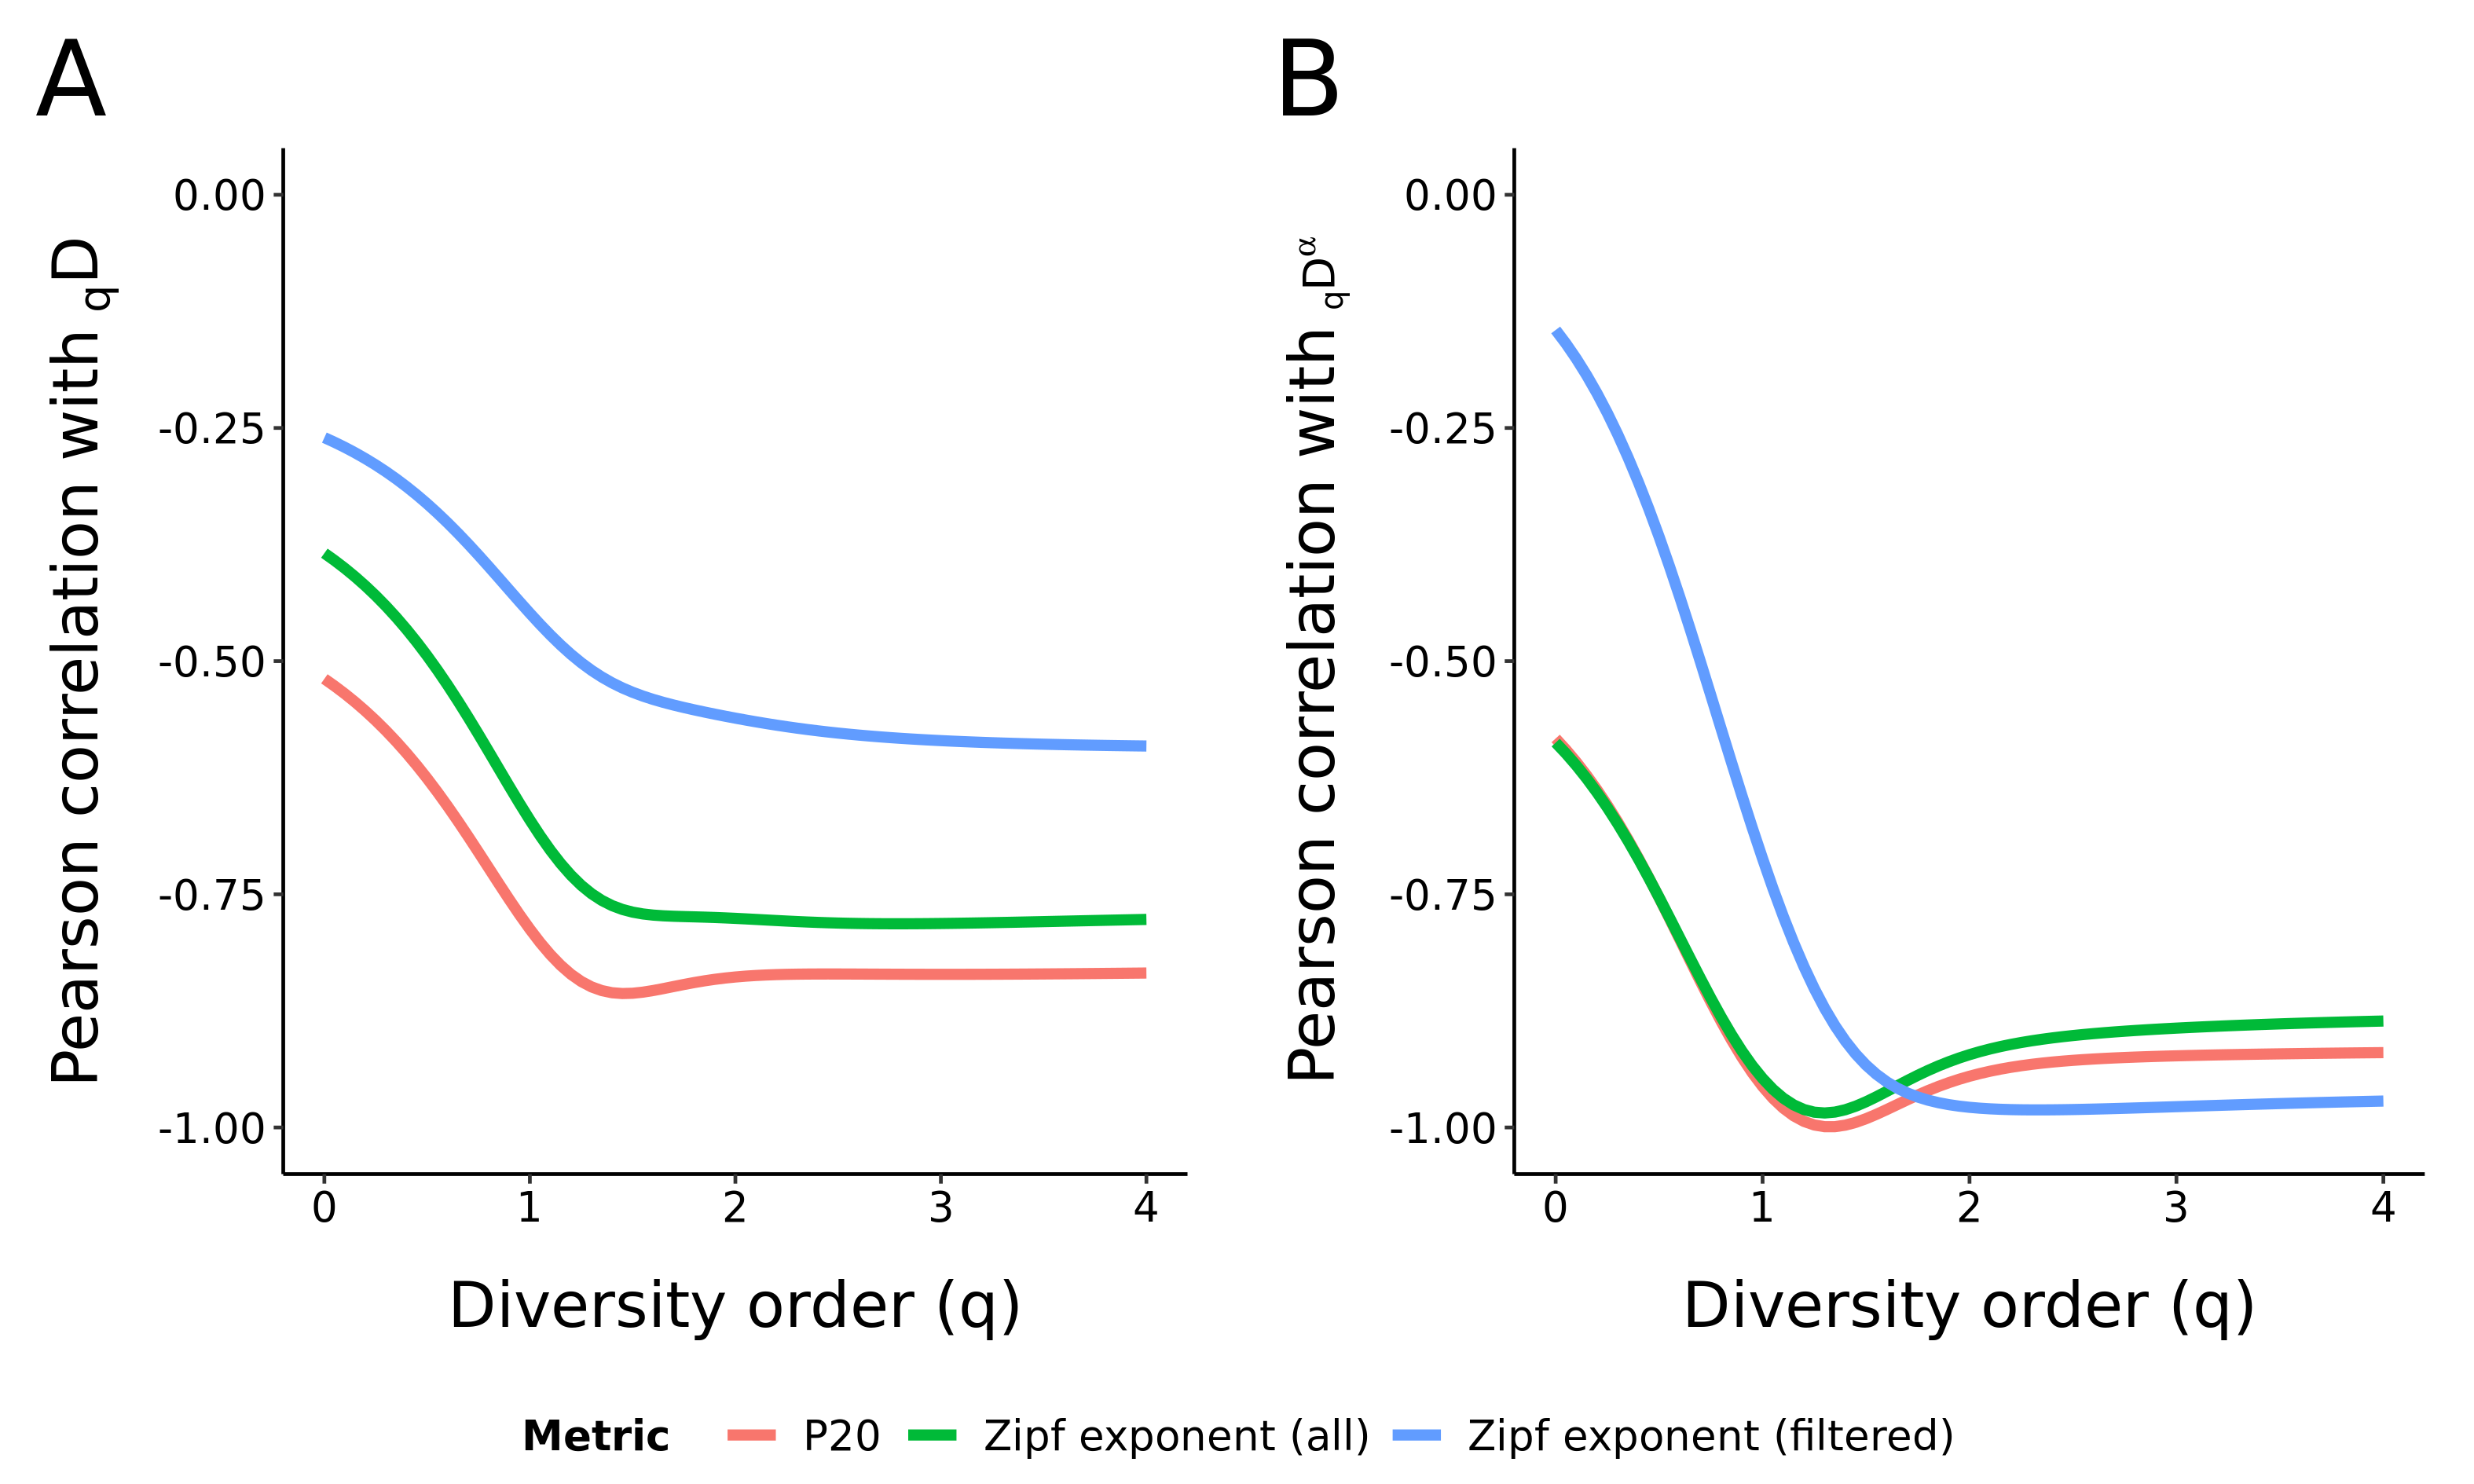
\includegraphics[width = 0.8\textwidth]{_Figures/png/pilot-clone-diversity-metrics-cor}
\caption[Correlation between Hill diversity and proxy metrics of clonal expansion]{\textbf{Correlation between Hill diversity and proxy metrics of clonal expansion:}
Pearson product-moment correlation coefficients between clonal Hill diversity and various proxy metrics (P20, fitted Zipf exponent over all clones, fitted Zipf exponent excluding largest clones) over a range of diversity orders for the \igseq pilot dataset. (A) Per-replicate correlation between proxy metrics and per-replicate diversity. (B) Per-individual correlation between averaged proxy metrics and alpha-diversity.}
\label{fig:igseq-pilot-clone-diversity-metrics-cor}
\end{figure}


\subsection{V(D)J segment usage and segment-repertoire diversity}
\label{sec:igseq_pilot_segments}

The clonal repertoire of an organism reflects the history of \naive B-cell production and subsequent clonal expansion in that individual, and as such is unique to each individual repertoire: by definition, clones cannot be shared between individuals. As such, while an essential part of any repertoire analysis (and a useful way to assess reproducibility between replicates), clonal measures are limited in their ability to meaningfully compare the antibody repertoires of different individuals. In contrast, the range of V(D)J-combinations available within an antibody repertoire is defined by the corresponding gene locus (\Cref{sec:nfu-locus}), and is therefore largely shared across individuals of a given species. This is particularly true for inbred lines of laboratory model organisms, for which the high level of polymorphism observed in the V-regions of wild populations \parencite{gadalamaria2015tigger,corcoran2016igdiscover} is not an issue. As such, the V(D)J usage distributions of antibody repertoires represent an alternative metric for measuring repertoire composition and diversity, which is more amenable to comparison between individuals (and groups of individuals) of the same species.

In order to analyse the composition of the V(D)J segment repertoire in an individual, we need unambiguous segment calls for as many unique sequences in that repertoire as possible. In the processed pilot dataset, \embed{_Figures/txt/pilot-segments-one-vj-n-pc.txt}\,\% of unique sequences (corresponding to \embed{_Figures/txt/pilot-segments-one-vj-conscount-pc.txt}\,\% of surviving input reads) were assigned an unambiguous VJ-identity, while only \embed{_Figures/txt/pilot-segments-one-vdj-n-pc.txt}\,\% of unique sequences (corresponding to \embed{_Figures/txt/pilot-segments-one-vdj-conscount-pc.txt}\,\% of surviving input reads) were assigned an unambiguous VDJ-identity. This difference arises from the fact that \embed{_Figures/txt/pilot-segments-ambig-d-n-pc.txt}\,\% of unique sequences (corresponding to \embed{_Figures/txt/pilot-segments-ambig-d-conscount-pc.txt}\,\% of surviving input reads) were assigned either no D-identity at all, or an ambiguous one with two or more possible D-assignments. To avoid any distortions or loss of resolution caused by the loss of almost a third of the dataset, I therefore proceed using the VJ-repertoire as ... % TODO: Finish this

\Cref{fig:igseq-pilot-vj-rank-frequency} shows the rank:frequency distribution of the VJ repertoire for each individual in the pilot dataset. Unlike with the clonal repertoire, these distributions are clearly not well-modelled by a power law even when the largest V/J combinations are excluded; in particular, the frequency of smaller V/J combinations declines much more quickly than would be predicted by Zipf's law. Nevertheless, these VJ repertoires are strongly dominated by the largest combinations in each individual, with P20 values ranging from \embed{_Figures/txt/pilot-segments-vj-p20-min.txt}\,\% to \embed{_Figures/txt/pilot-segments-vj-p20-max.txt}\,\%. In total, of the \embed{_Figures/txt/pilot-segments-vj-n-theoretical.txt} possible theoretically distinguishable V/J combinations in the turquoise-killifish repertoire, \embed{_Figures/txt/pilot-segments-vj-n-any.txt} (\embed{_Figures/txt/pilot-segments-vj-pc-any.txt}\,\%) are observed in at least one individual, with the number observed in any single individual ranging from \embed{_Figures/txt/pilot-segments-vj-n-min.txt} (\embed{_Figures/txt/pilot-segments-vj-pc-min.txt}\,\%) to \embed{_Figures/txt/pilot-segments-vj-n-max.txt} (\embed{_Figures/txt/pilot-segments-vj-pc-max.txt}\,\%).

\begin{figure}
\centering
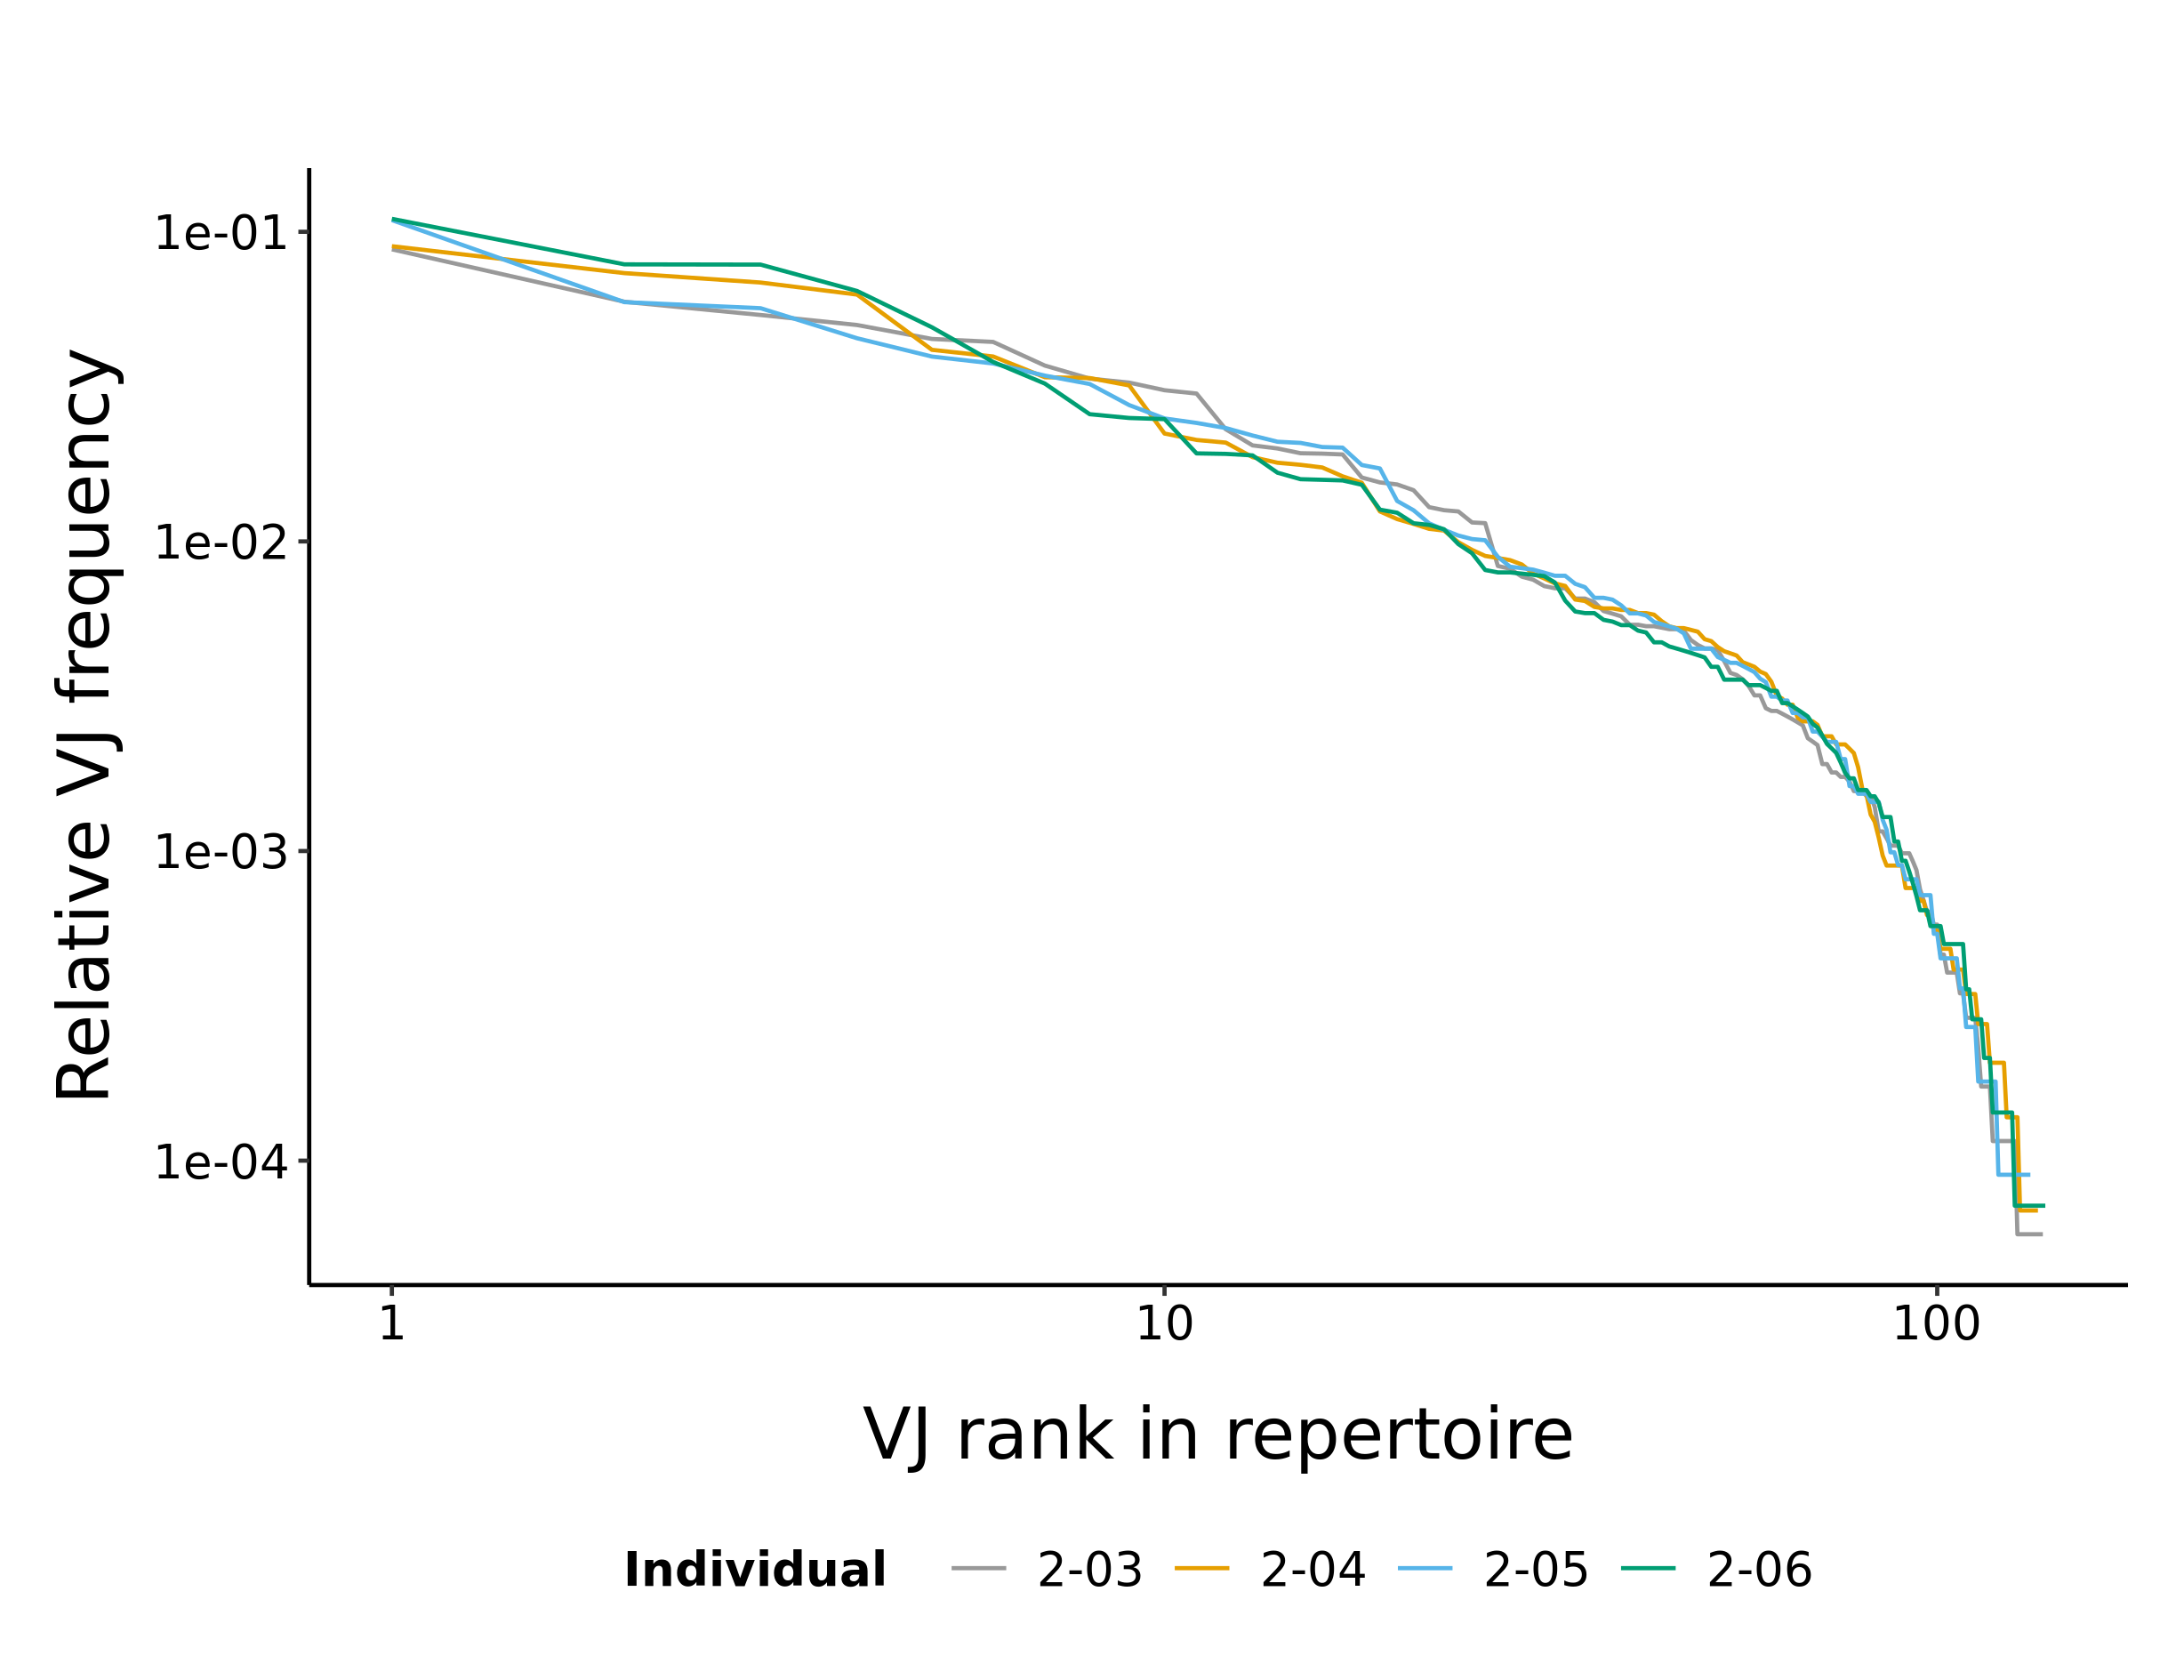
\includegraphics[width=0.8\textwidth]{_Figures/png/pilot-vj-rank-frequency}
\caption[Rank/frequency distributions of pilot VJ repertoires]{\textbf{Rank/frequency distributions of pilot VJ repertoires:} ...} % TODO: Fill in caption
\label{fig:igseq-pilot-vj-rank-frequency}
\end{figure}

As with the clonal repertoire, the diversity of the VJ repertoire can be assessed in a wide variety of ways, among the most flexible and informative of which is the Hill diversity spectrum (\Cref{app:diversity}). \Cref{fig:igseq-pilot-vj-diversity} shows the alpha (\Cref{fig:igseq-pilot-vj-diversity-alpha}) and beta (\Cref{fig:igseq-pilot-vj-diversity-beta}) diversity spectra of the VJ repertoire for each individual in the pilot dataset. As with the clonal repertoire, there were no significant pairwise differences in alpha diversity between individuals, although in this case a Kruskal-Wallis test was able to find a marginally significant overall effect of individual on VJ diversity at high diversity orders (\Cref{fig:igseq-pilot-clone-diversity-solo-box}); this difference probably arises from the fact that, for some individuals, the VJ-repertoire diversity spectra were much more similar between replicates of the same individual than in the clonal repertoire (\Cref{fig:igseq-pilot-vj-diversity-solo-spectra,fig:igseq-pilot-clone-diversity-solo-spectra}). 

\begin{figure}
\centering
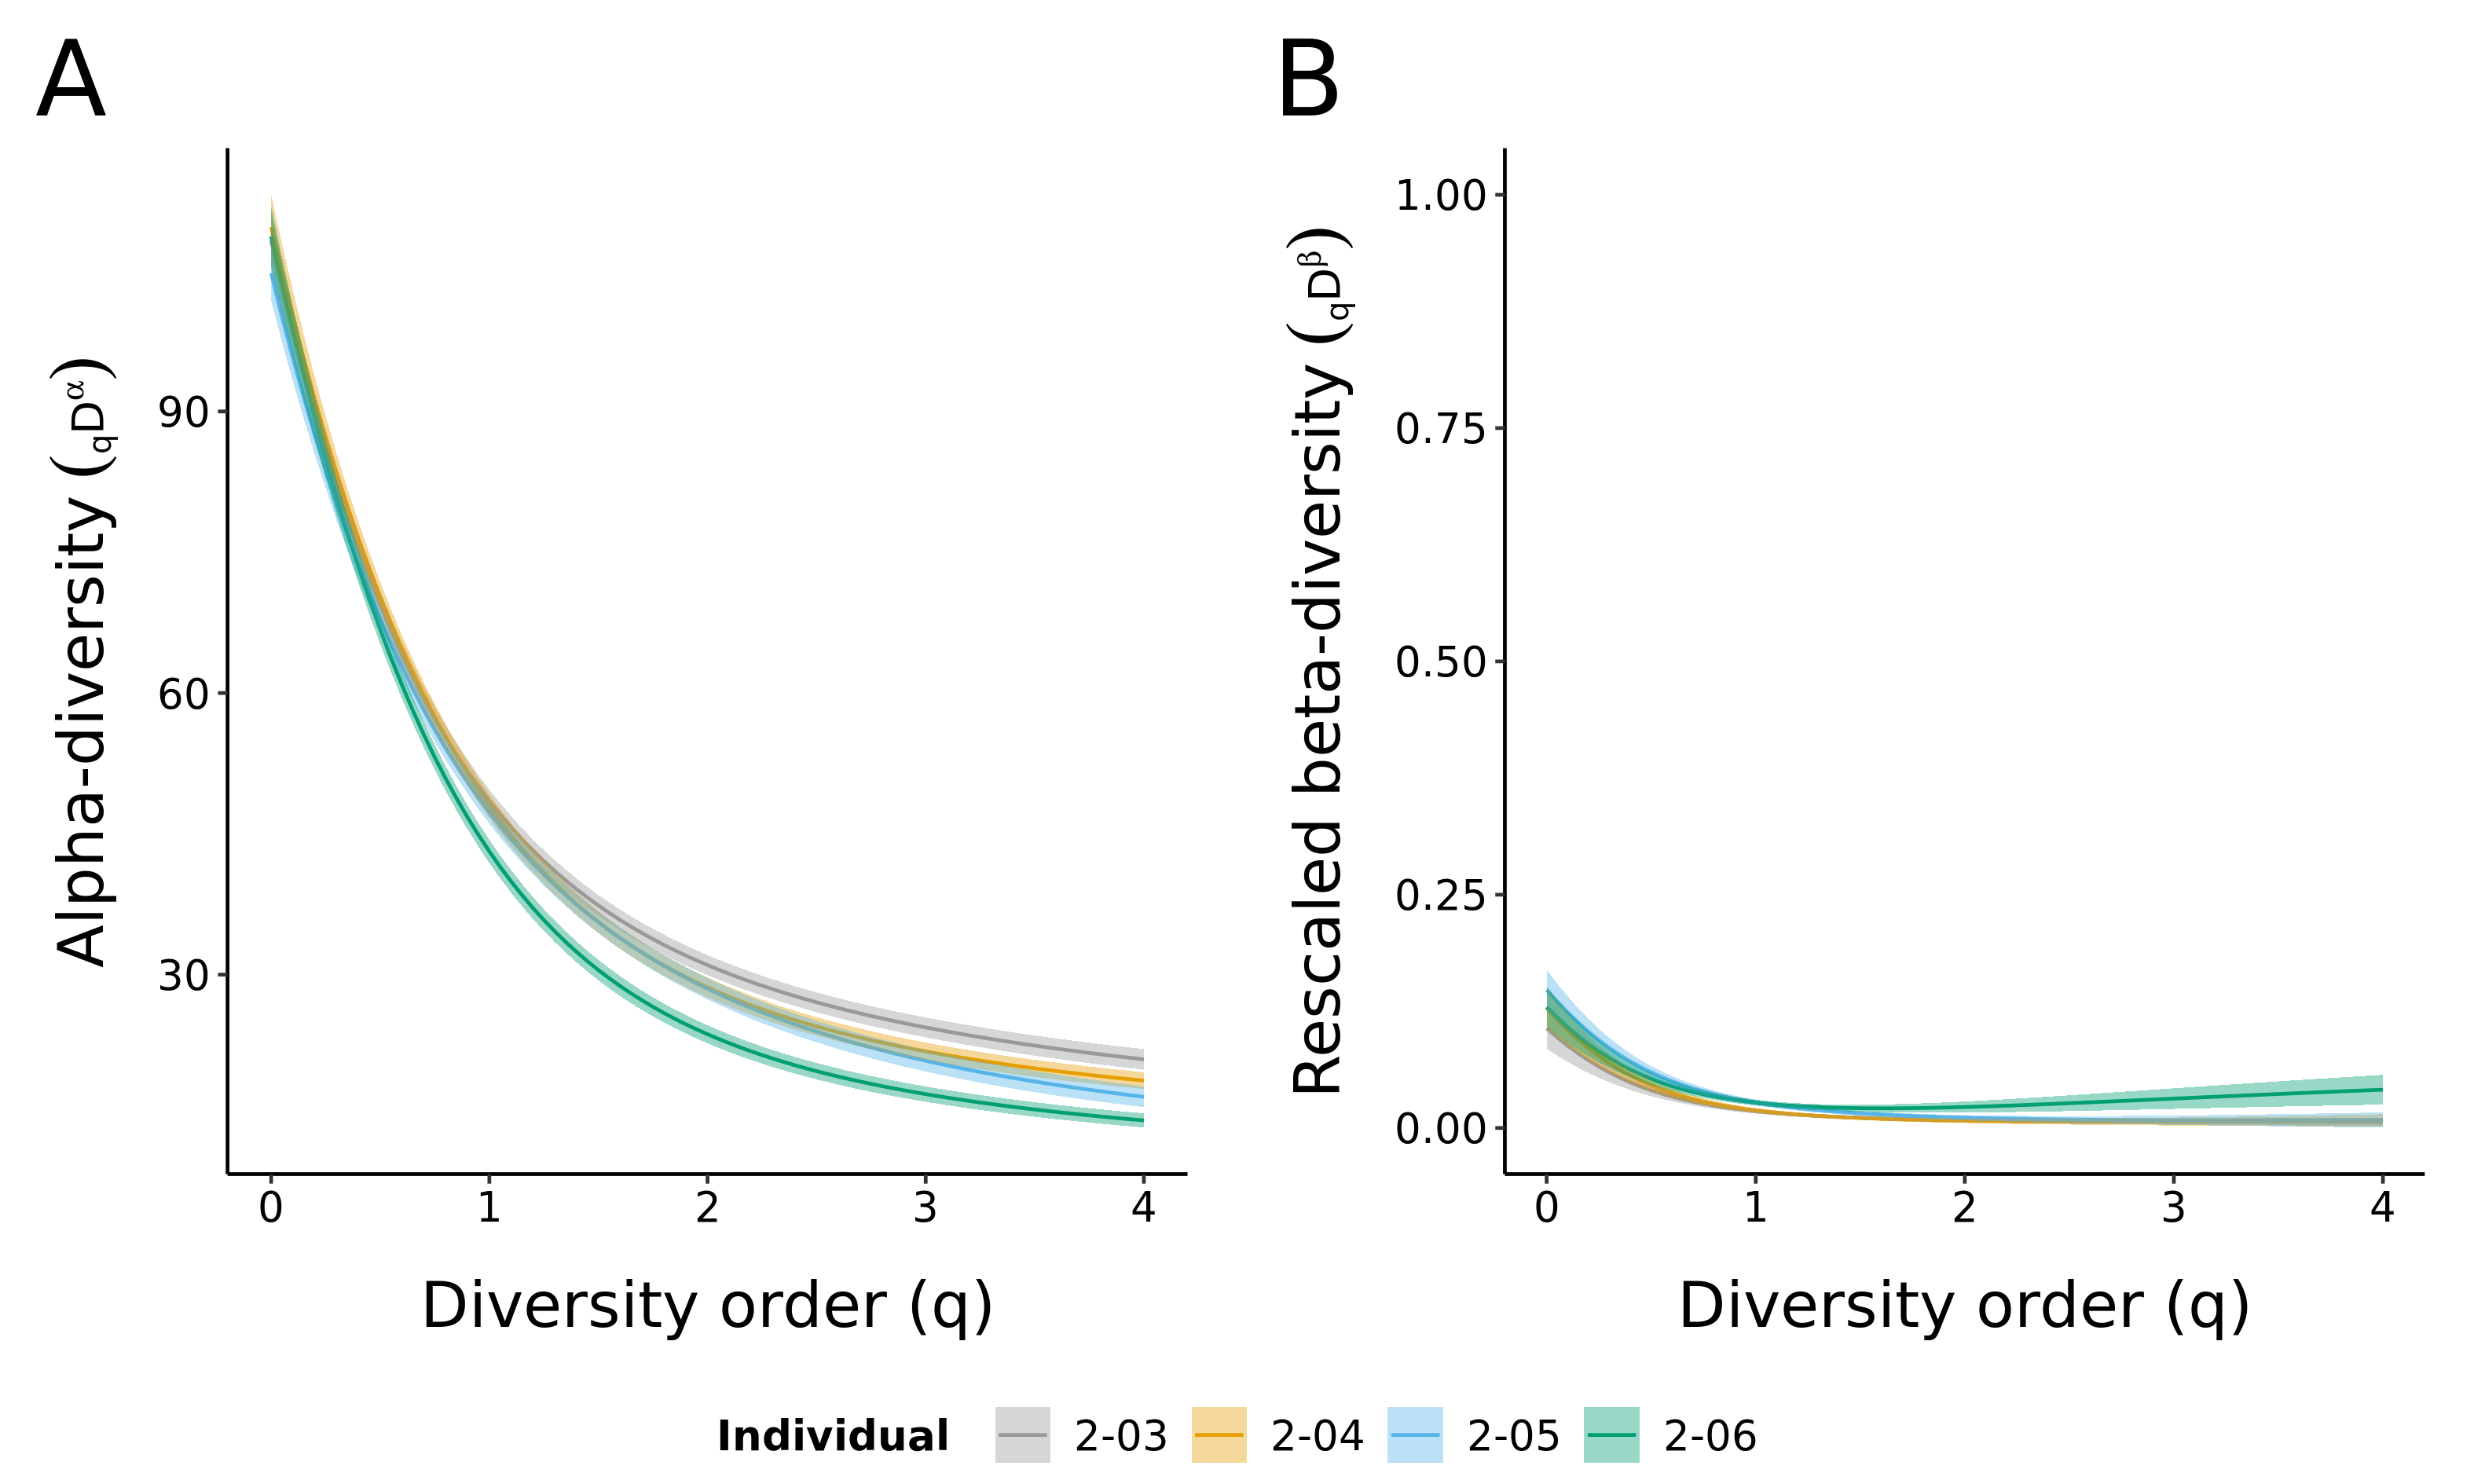
\includegraphics[width = 0.9\textwidth]{_Figures/png/pilot-vj-diversity}
\begin{subfigure}{0em}
\phantomsubcaption{}
\label{fig:igseq-pilot-vj-diversity-alpha}
\end{subfigure}
\begin{subfigure}{0em}
\phantomsubcaption{}
\label{fig:igseq-pilot-vj-diversity-beta}
\end{subfigure}
\caption{\textbf{VJ-diversity spectra for pilot dataset:} Hill diversity spectra of VJ usage (as measured by number of unique sequences per V/J combination) over replicates for each individual in the pilot dataset. (A) Alpha-diversity across replicates; (B) Beta-diversity across replicates, rescaled to between 0 (minimum) and 1 (maximum) for each individual. Shaded regions in both subfigures represent 95\,\% confidence intervals, estimated using bootstrapping.} % TODO: Parametric or nonparametric?
\label{fig:igseq-pilot-vj-diversity}
\end{figure}

\begin{figure}
\centering
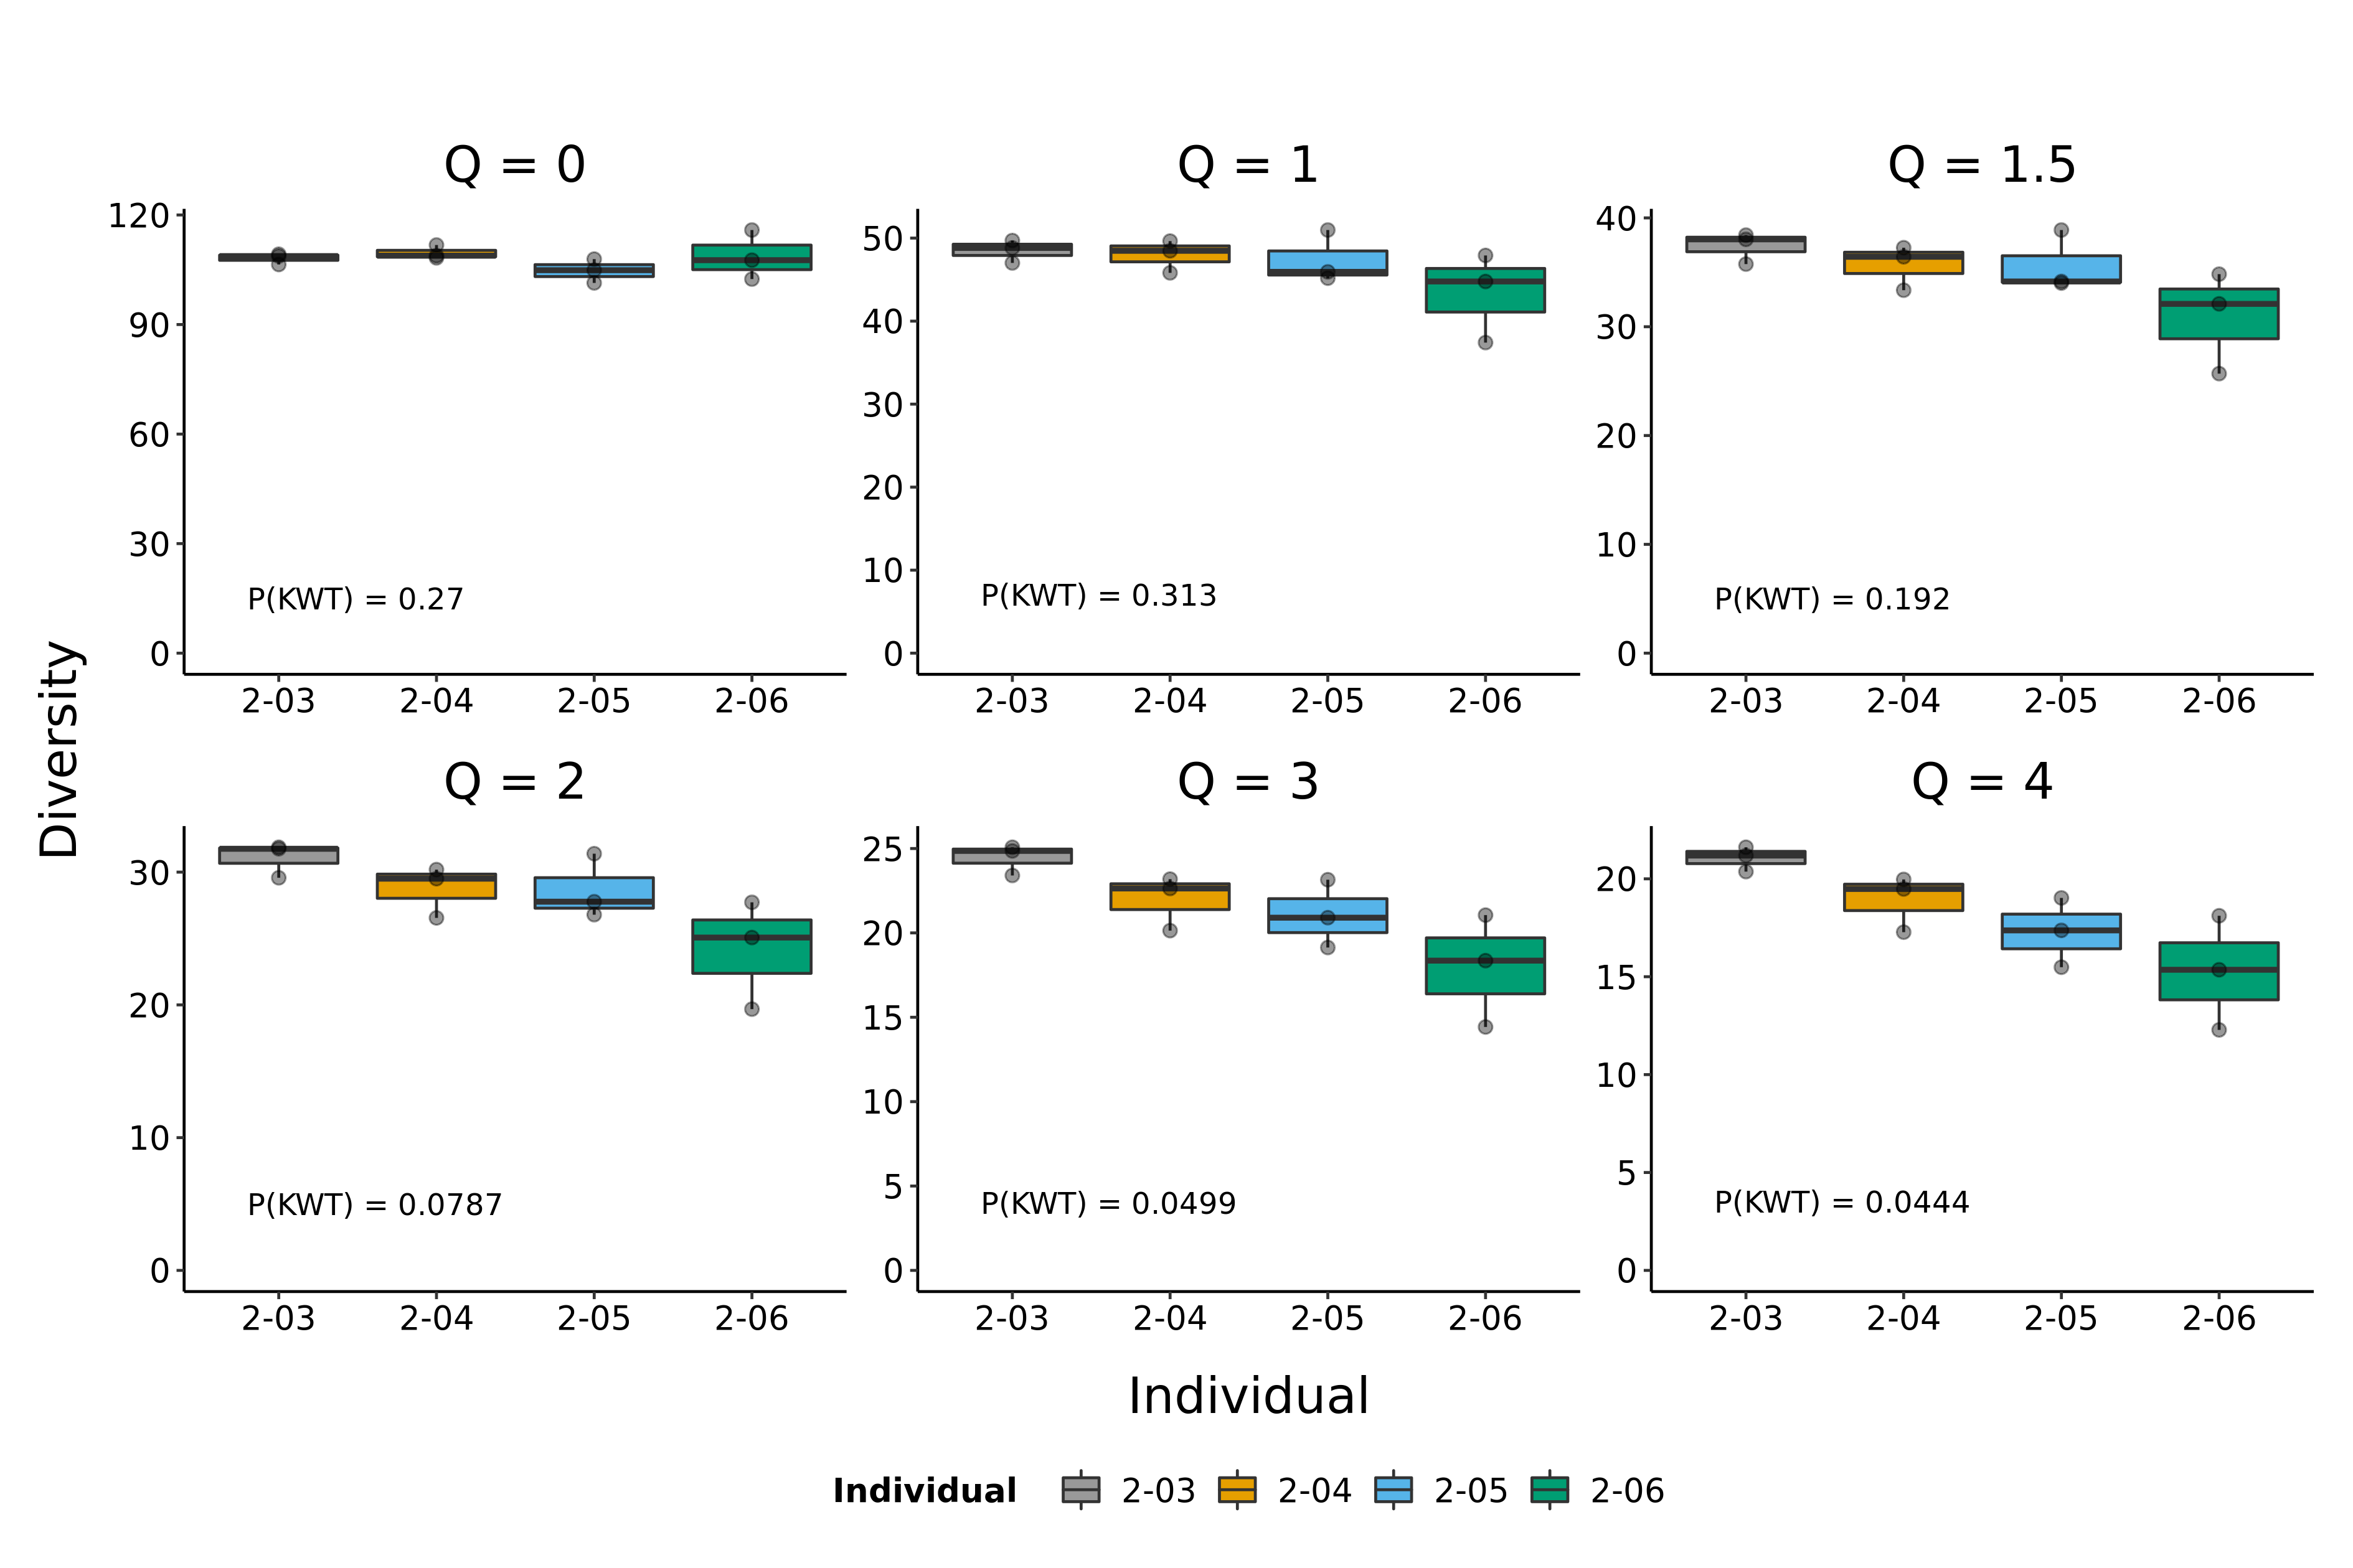
\includegraphics[width = 0.8\textwidth]{_Figures/png/pilot-vj-diversity-solo-box}
\caption{Boxplots of Hill diversity values for the VJ repertoires of replicates from each individual in the \igseq pilot dataset at a sample of diversity orders. Pairwise $p$-values are computed using nonparametric Mann–Whitney U tests ($*: 0.01 < p \leq 0.05;~**: 0.001 < p \leq 0.01;~***: p \leq 0.001$). Annotated $p$-values ($P(KWT)$) indicates the statistical significance of the estimated individual effect on diversity at each order under a Kruskal-Wallis test.} % TODO: Figure title
\label{fig:igseq-pilot-clone-diversity-solo-box}
\end{figure}

The beta-diversity spectra, meanwhile, are close to the minimum value across all diversity orders, indicating that the V/J usage distribution in each individual's secondary repertoire is highly consistent across replicates for both large and small V/J combinations. To verify that this low beta-diversity is the result of replicability between replicates, rather than homogeneity in V/J usage between individuals, I made use of the Repertoire Dissimilarity Index (RDI) \parencite{bolen2017rdi}, a method for computing a distance between any two repertoires based on the Euclidean distance between their respective V(D)J-abundance vectors (\Cref{sec:methods_comp_igdownstream_rdi}). Average-linkage clustering on the basis of the VJ-RDI distances between replicates in the pilot dataset correctly re-groups all replicates from all four individuals (\Cref{fig:igseq-pilot-rdi-dendrogram}), demonstrating that the information in the VJ repertoire is sufficient to distinguish repertoires from different individuals.

\begin{figure}
\centering
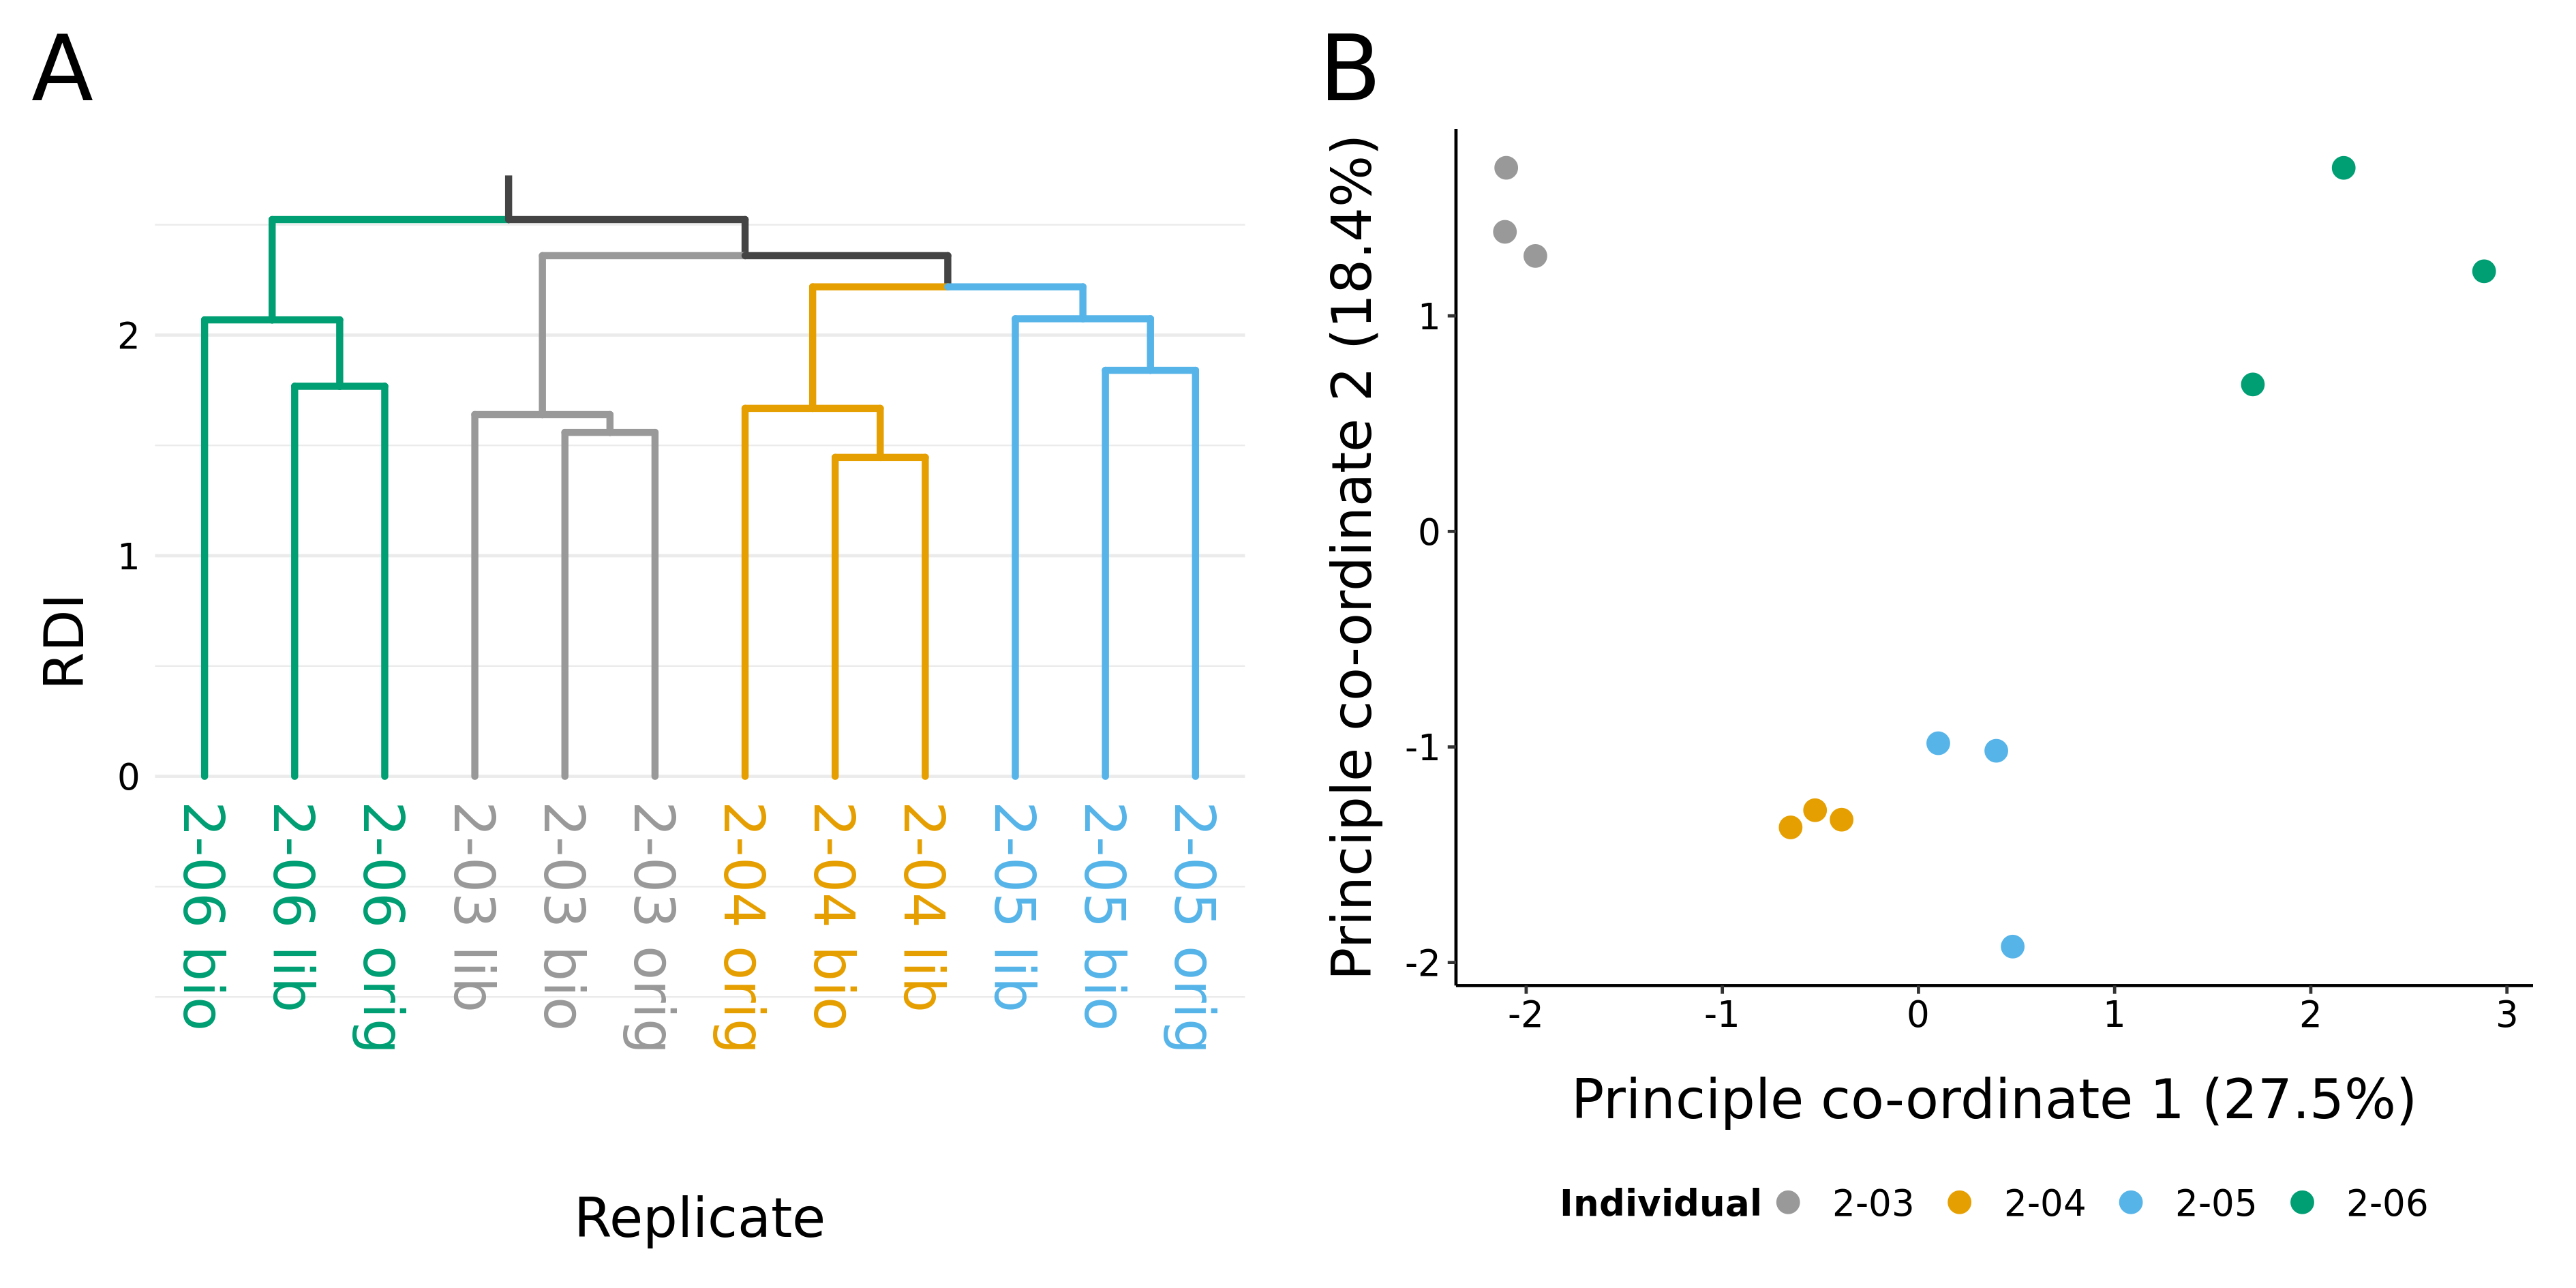
\includegraphics[width = 0.9\textwidth]{_Figures/png/pilot-rdi-vj-replicate}
\begin{subfigure}{0em}
\phantomsubcaption{}
\label{fig:igseq-pilot-rdi-dendrogram}
\end{subfigure}
\begin{subfigure}{0em}
\phantomsubcaption{}
\label{fig:igseq-pilot-rdi-pcoa}
\end{subfigure}
\caption[Repertoire dissimilarity index (RDI) analysis of pilot data]{\textbf{Repertoire dissimilarity index (RDI) analysis of pilot data:} (A) Dendrogram of pilot replicates produced through average-linkage clustering on pairwise VJ-RDI distances. (B) Principal co-ordinate analysis (PCoA) of pairwise VJ-RDI distances between pilot replicates, coloured by source individual.}
\label{fig:igseq-pilot-rdi}
\end{figure}

% TODO: Add (or abandon) IGoR section here
\dots

\FloatBarrier
\clearpage